% Options for packages loaded elsewhere
\PassOptionsToPackage{unicode}{hyperref}
\PassOptionsToPackage{hyphens}{url}
%
\documentclass[
]{article}
\usepackage{lmodern}
\usepackage{amssymb,amsmath}
\usepackage{ifxetex,ifluatex}
\ifnum 0\ifxetex 1\fi\ifluatex 1\fi=0 % if pdftex
  \usepackage[T1]{fontenc}
  \usepackage[utf8]{inputenc}
  \usepackage{textcomp} % provide euro and other symbols
\else % if luatex or xetex
  \usepackage{unicode-math}
  \defaultfontfeatures{Scale=MatchLowercase}
  \defaultfontfeatures[\rmfamily]{Ligatures=TeX,Scale=1}
\fi
% Use upquote if available, for straight quotes in verbatim environments
\IfFileExists{upquote.sty}{\usepackage{upquote}}{}
\IfFileExists{microtype.sty}{% use microtype if available
  \usepackage[]{microtype}
  \UseMicrotypeSet[protrusion]{basicmath} % disable protrusion for tt fonts
}{}
\makeatletter
\@ifundefined{KOMAClassName}{% if non-KOMA class
  \IfFileExists{parskip.sty}{%
    \usepackage{parskip}
  }{% else
    \setlength{\parindent}{0pt}
    \setlength{\parskip}{6pt plus 2pt minus 1pt}}
}{% if KOMA class
  \KOMAoptions{parskip=half}}
\makeatother
\usepackage{xcolor}
\IfFileExists{xurl.sty}{\usepackage{xurl}}{} % add URL line breaks if available
\IfFileExists{bookmark.sty}{\usepackage{bookmark}}{\usepackage{hyperref}}
\hypersetup{
  pdftitle={Tarea 2},
  hidelinks,
  pdfcreator={LaTeX via pandoc}}
\urlstyle{same} % disable monospaced font for URLs
\usepackage[margin=1in]{geometry}
\usepackage{color}
\usepackage{fancyvrb}
\newcommand{\VerbBar}{|}
\newcommand{\VERB}{\Verb[commandchars=\\\{\}]}
\DefineVerbatimEnvironment{Highlighting}{Verbatim}{commandchars=\\\{\}}
% Add ',fontsize=\small' for more characters per line
\usepackage{framed}
\definecolor{shadecolor}{RGB}{248,248,248}
\newenvironment{Shaded}{\begin{snugshade}}{\end{snugshade}}
\newcommand{\AlertTok}[1]{\textcolor[rgb]{0.94,0.16,0.16}{#1}}
\newcommand{\AnnotationTok}[1]{\textcolor[rgb]{0.56,0.35,0.01}{\textbf{\textit{#1}}}}
\newcommand{\AttributeTok}[1]{\textcolor[rgb]{0.77,0.63,0.00}{#1}}
\newcommand{\BaseNTok}[1]{\textcolor[rgb]{0.00,0.00,0.81}{#1}}
\newcommand{\BuiltInTok}[1]{#1}
\newcommand{\CharTok}[1]{\textcolor[rgb]{0.31,0.60,0.02}{#1}}
\newcommand{\CommentTok}[1]{\textcolor[rgb]{0.56,0.35,0.01}{\textit{#1}}}
\newcommand{\CommentVarTok}[1]{\textcolor[rgb]{0.56,0.35,0.01}{\textbf{\textit{#1}}}}
\newcommand{\ConstantTok}[1]{\textcolor[rgb]{0.00,0.00,0.00}{#1}}
\newcommand{\ControlFlowTok}[1]{\textcolor[rgb]{0.13,0.29,0.53}{\textbf{#1}}}
\newcommand{\DataTypeTok}[1]{\textcolor[rgb]{0.13,0.29,0.53}{#1}}
\newcommand{\DecValTok}[1]{\textcolor[rgb]{0.00,0.00,0.81}{#1}}
\newcommand{\DocumentationTok}[1]{\textcolor[rgb]{0.56,0.35,0.01}{\textbf{\textit{#1}}}}
\newcommand{\ErrorTok}[1]{\textcolor[rgb]{0.64,0.00,0.00}{\textbf{#1}}}
\newcommand{\ExtensionTok}[1]{#1}
\newcommand{\FloatTok}[1]{\textcolor[rgb]{0.00,0.00,0.81}{#1}}
\newcommand{\FunctionTok}[1]{\textcolor[rgb]{0.00,0.00,0.00}{#1}}
\newcommand{\ImportTok}[1]{#1}
\newcommand{\InformationTok}[1]{\textcolor[rgb]{0.56,0.35,0.01}{\textbf{\textit{#1}}}}
\newcommand{\KeywordTok}[1]{\textcolor[rgb]{0.13,0.29,0.53}{\textbf{#1}}}
\newcommand{\NormalTok}[1]{#1}
\newcommand{\OperatorTok}[1]{\textcolor[rgb]{0.81,0.36,0.00}{\textbf{#1}}}
\newcommand{\OtherTok}[1]{\textcolor[rgb]{0.56,0.35,0.01}{#1}}
\newcommand{\PreprocessorTok}[1]{\textcolor[rgb]{0.56,0.35,0.01}{\textit{#1}}}
\newcommand{\RegionMarkerTok}[1]{#1}
\newcommand{\SpecialCharTok}[1]{\textcolor[rgb]{0.00,0.00,0.00}{#1}}
\newcommand{\SpecialStringTok}[1]{\textcolor[rgb]{0.31,0.60,0.02}{#1}}
\newcommand{\StringTok}[1]{\textcolor[rgb]{0.31,0.60,0.02}{#1}}
\newcommand{\VariableTok}[1]{\textcolor[rgb]{0.00,0.00,0.00}{#1}}
\newcommand{\VerbatimStringTok}[1]{\textcolor[rgb]{0.31,0.60,0.02}{#1}}
\newcommand{\WarningTok}[1]{\textcolor[rgb]{0.56,0.35,0.01}{\textbf{\textit{#1}}}}
\usepackage{graphicx,grffile}
\makeatletter
\def\maxwidth{\ifdim\Gin@nat@width>\linewidth\linewidth\else\Gin@nat@width\fi}
\def\maxheight{\ifdim\Gin@nat@height>\textheight\textheight\else\Gin@nat@height\fi}
\makeatother
% Scale images if necessary, so that they will not overflow the page
% margins by default, and it is still possible to overwrite the defaults
% using explicit options in \includegraphics[width, height, ...]{}
\setkeys{Gin}{width=\maxwidth,height=\maxheight,keepaspectratio}
% Set default figure placement to htbp
\makeatletter
\def\fps@figure{htbp}
\makeatother
\setlength{\emergencystretch}{3em} % prevent overfull lines
\providecommand{\tightlist}{%
  \setlength{\itemsep}{0pt}\setlength{\parskip}{0pt}}
\setcounter{secnumdepth}{-\maxdimen} % remove section numbering

\title{Tarea 2}
\author{}
\date{\vspace{-2.5em}}

\begin{document}
\maketitle

\hypertarget{pregunta-1}{%
\subsubsection{\texorpdfstring{\textbf{Pregunta
1}}{Pregunta 1}}\label{pregunta-1}}

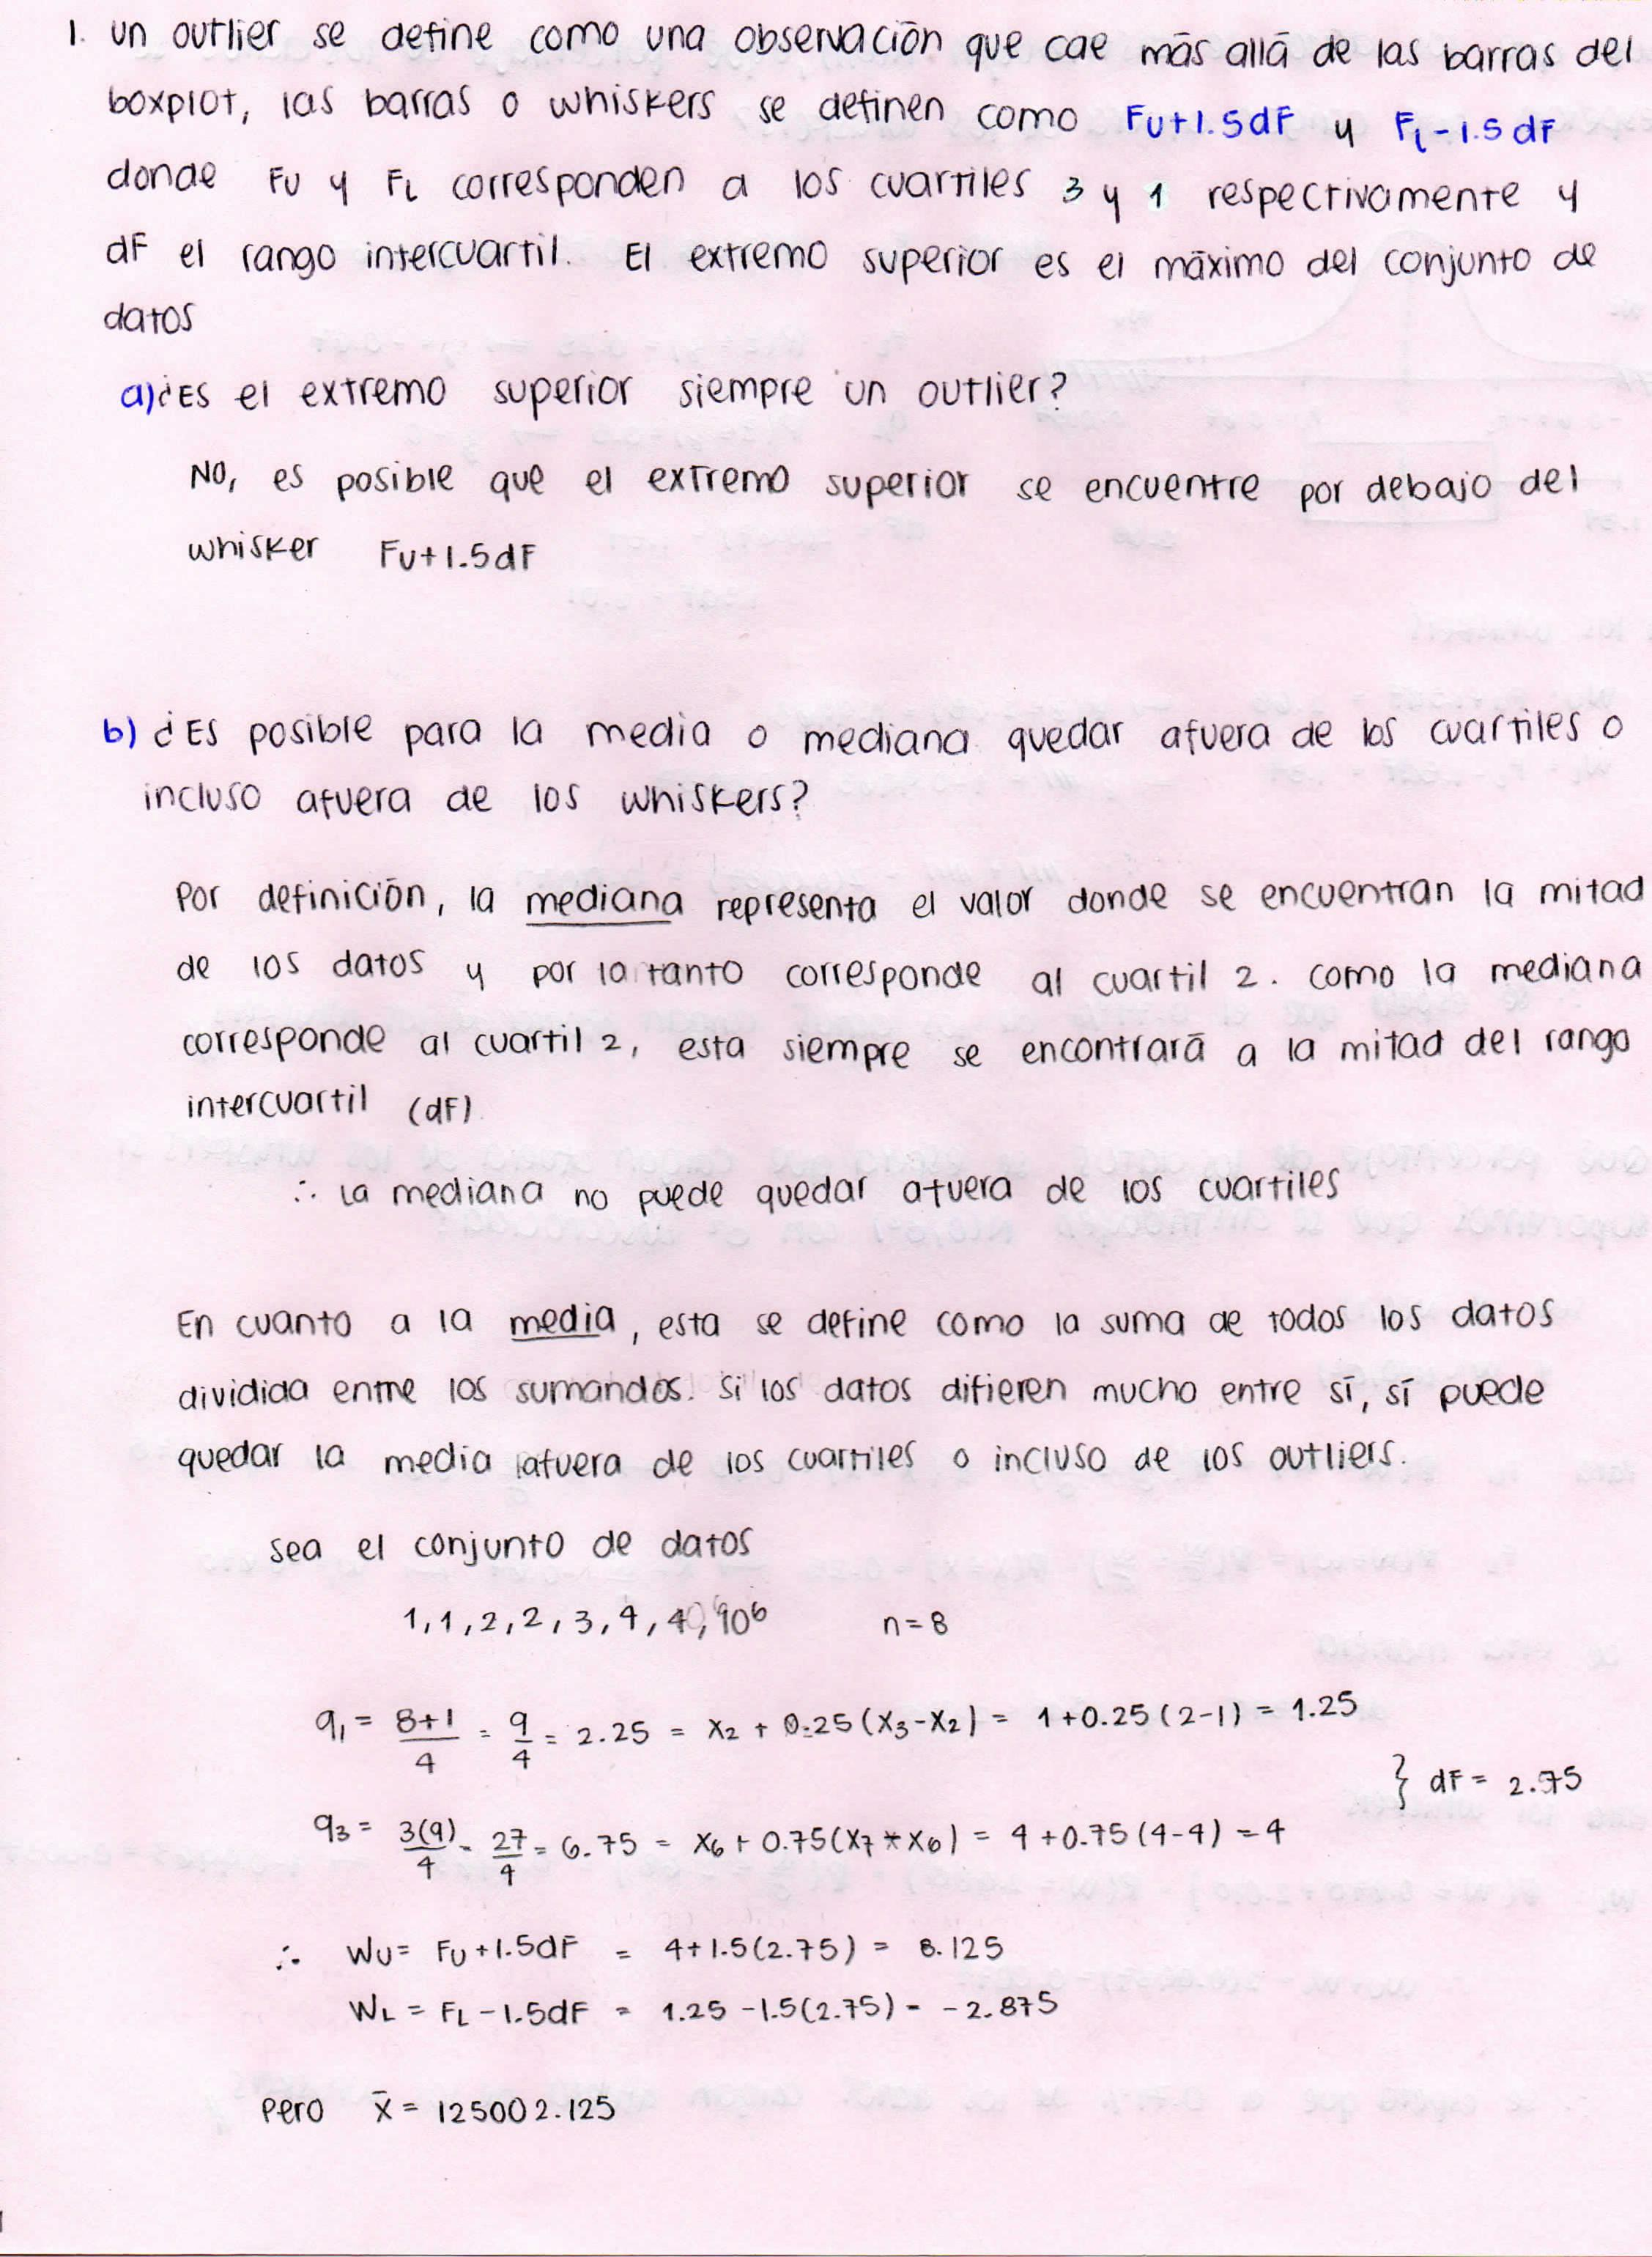
\includegraphics{1a.jpg}

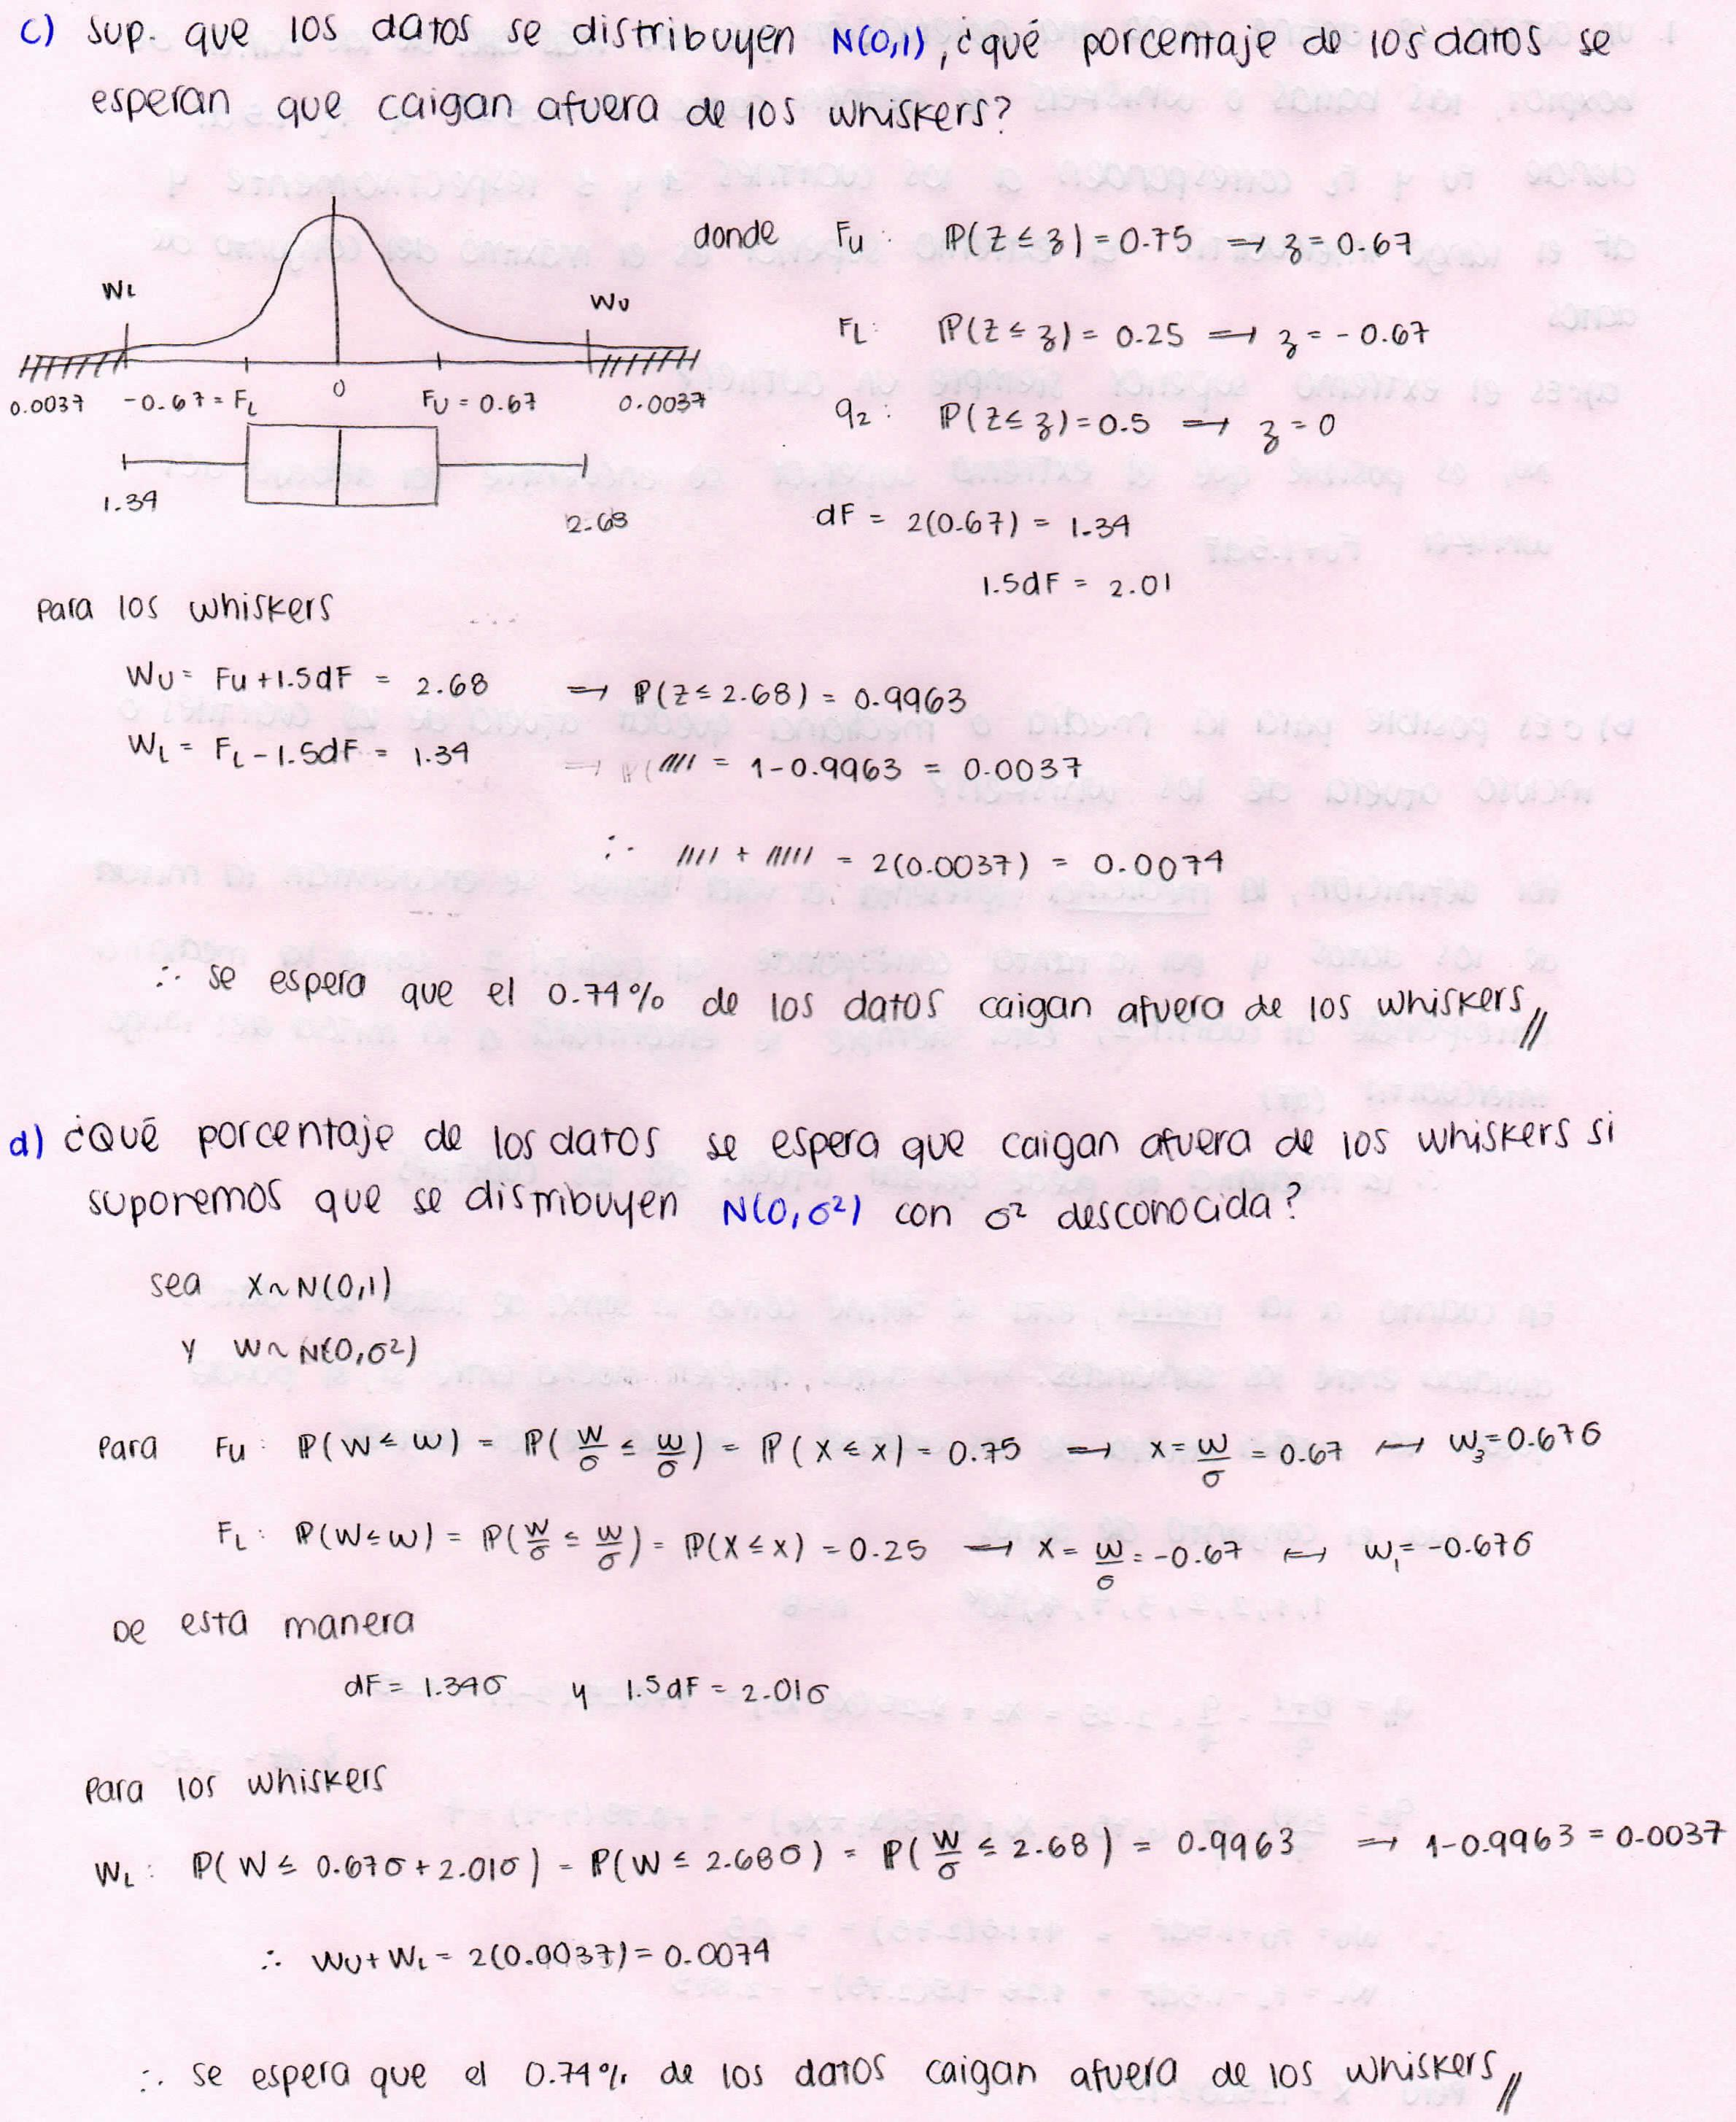
\includegraphics{1b.jpg}

\textbf{2. 50 observaciones de una \(\mathcal{N}(0,1)\) y otras 50
observaciones de una \(\mathcal{N}(2,1)\). ¿Cómo se verán las 100 caras
de Chernoff si \(X\) y \(Y\) definen la línea de la cara y la oscuridad
del cabello?, ¿esperan caras similares?, ¿cuántas caras lucen como
oservaciones de \(Y\) cuando aún son observaciones de \(X\)?}

\begin{Shaded}
\begin{Highlighting}[]
\NormalTok{  ind      =}\StringTok{ }\KeywordTok{matrix}\NormalTok{(}\DecValTok{0}\NormalTok{, }\DataTypeTok{ncol =} \DecValTok{36}\NormalTok{)   }\CommentTok{# define una indicadora para el argumento which.row}
\NormalTok{  ind[,}\DecValTok{13}\NormalTok{] =}\StringTok{ }\DecValTok{1}                      \CommentTok{# linea derecha de la cara}
\NormalTok{  ind[,}\DecValTok{14}\NormalTok{] =}\StringTok{ }\DecValTok{1}                      \CommentTok{# oscuridad del cabello lado derecho}
\NormalTok{  ind[,}\DecValTok{31}\NormalTok{] =}\StringTok{ }\DecValTok{1}                      \CommentTok{# linea izquierda de la cara}
\NormalTok{  ind[,}\DecValTok{32}\NormalTok{] =}\StringTok{ }\DecValTok{1}                      \CommentTok{# oscuridad izquierda del cabello}
\NormalTok{  x      =}\StringTok{ }\KeywordTok{rnorm}\NormalTok{(}\DecValTok{50}\NormalTok{)               }
\NormalTok{  y      =}\StringTok{ }\KeywordTok{rnorm}\NormalTok{(}\DecValTok{50}\NormalTok{, }\DataTypeTok{mean =} \DecValTok{2}\NormalTok{) }
\NormalTok{  z      =}\StringTok{ }\KeywordTok{t}\NormalTok{(}\KeywordTok{cbind}\NormalTok{(}\KeywordTok{t}\NormalTok{(x),}\KeywordTok{t}\NormalTok{(y)));    }\CommentTok{# arma matriz (100x1)}
  \KeywordTok{faces}\NormalTok{(}\KeywordTok{as.matrix}\NormalTok{(z[}\DecValTok{1}\OperatorTok{:}\DecValTok{50}\NormalTok{]),ind, }\DataTypeTok{main=}\StringTok{"Observaciones 1 a 50"}\NormalTok{, }\DataTypeTok{ncol.plot =} \DecValTok{5}\NormalTok{, }\DataTypeTok{nrow.plot =} \DecValTok{10}\NormalTok{) }\CommentTok{# primeras 50 caras}
\end{Highlighting}
\end{Shaded}

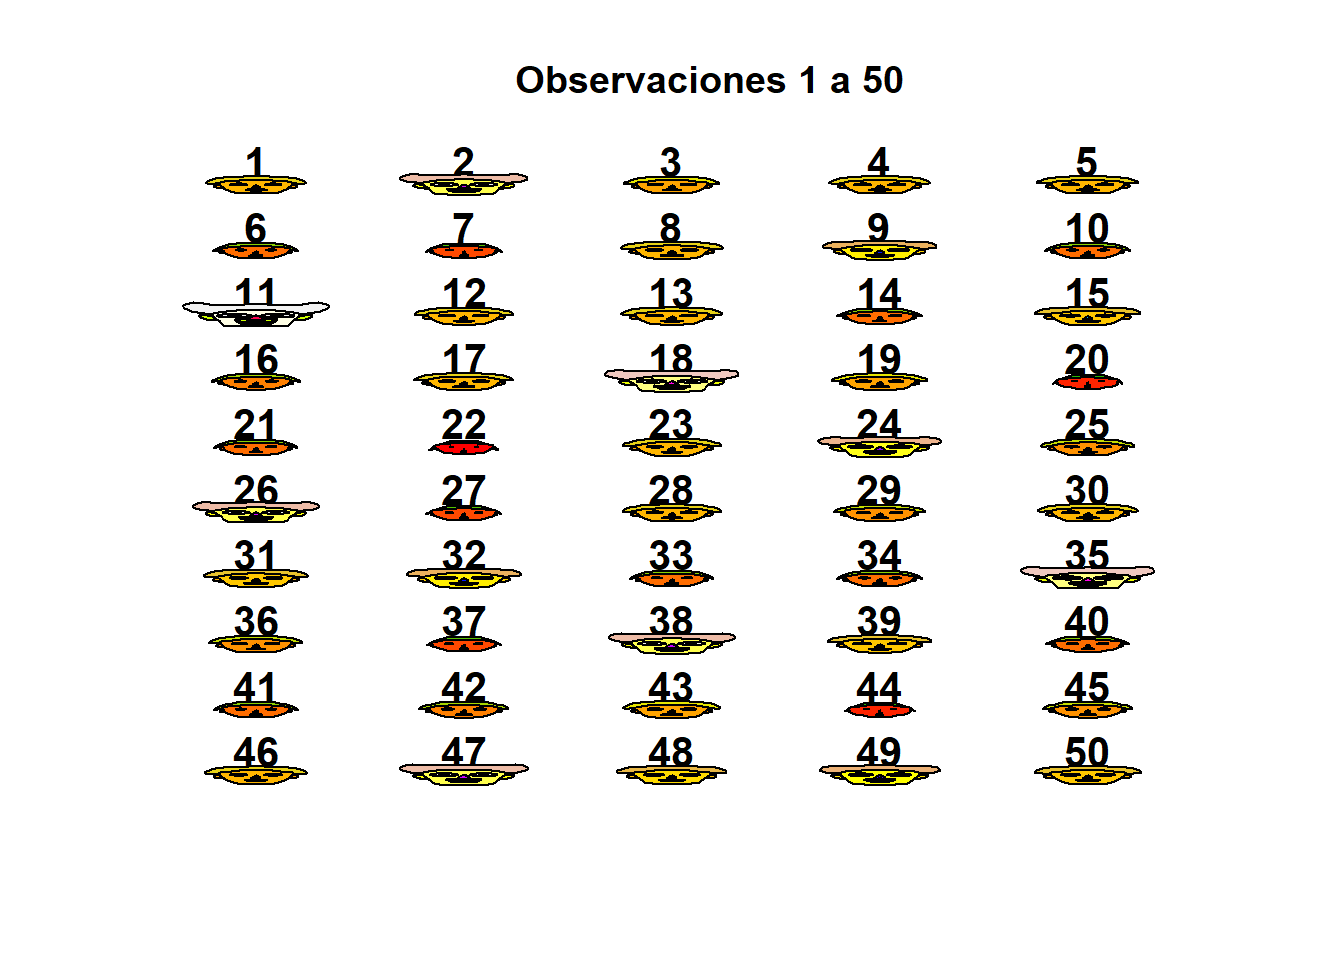
\includegraphics{Tarea-2_files/figure-latex/unnamed-chunk-2-1.pdf}

\begin{verbatim}
## effect of variables:
##  modified item       Var   
##  "height of face   " "Var1"
##  "width of face    " "Var1"
##  "structure of face" "Var1"
##  "height of mouth  " "Var1"
##  "width of mouth   " "Var1"
##  "smiling          " "Var1"
##  "height of eyes   " "Var1"
##  "width of eyes    " "Var1"
##  "height of hair   " "Var1"
##  "width of hair   "  "Var1"
##  "style of hair   "  "Var1"
##  "height of nose  "  "Var1"
##  "width of nose   "  "Var1"
##  "width of ear    "  "Var1"
##  "height of ear   "  "Var1"
\end{verbatim}

\begin{Shaded}
\begin{Highlighting}[]
  \KeywordTok{faces}\NormalTok{(}\KeywordTok{as.matrix}\NormalTok{(z[}\DecValTok{51}\OperatorTok{:}\DecValTok{100}\NormalTok{]),ind, }\DataTypeTok{main=}\StringTok{"Observaciones 51 a 100"}\NormalTok{, }\DataTypeTok{ncol.plot =} \DecValTok{5}\NormalTok{, }\DataTypeTok{nrow.plot =} \DecValTok{10}\NormalTok{) }\CommentTok{# primeras 50 caras}
\end{Highlighting}
\end{Shaded}

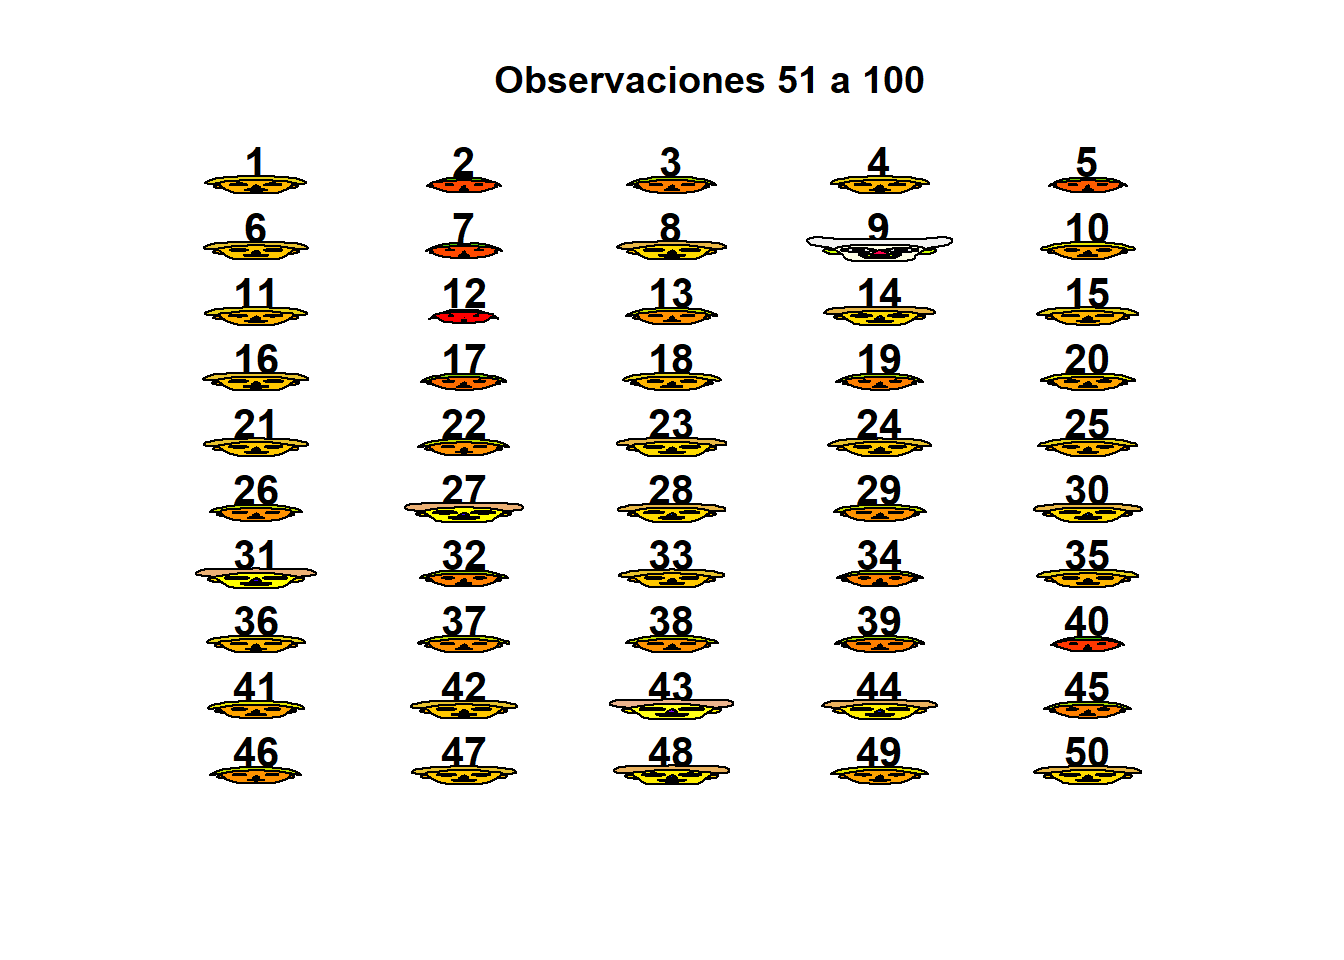
\includegraphics{Tarea-2_files/figure-latex/unnamed-chunk-2-2.pdf}

\begin{verbatim}
## effect of variables:
##  modified item       Var   
##  "height of face   " "Var1"
##  "width of face    " "Var1"
##  "structure of face" "Var1"
##  "height of mouth  " "Var1"
##  "width of mouth   " "Var1"
##  "smiling          " "Var1"
##  "height of eyes   " "Var1"
##  "width of eyes    " "Var1"
##  "height of hair   " "Var1"
##  "width of hair   "  "Var1"
##  "style of hair   "  "Var1"
##  "height of nose  "  "Var1"
##  "width of nose   "  "Var1"
##  "width of ear    "  "Var1"
##  "height of ear   "  "Var1"
\end{verbatim}

\begin{Shaded}
\begin{Highlighting}[]
\NormalTok{  x}
\end{Highlighting}
\end{Shaded}

\begin{verbatim}
##  [1]  0.30747631 -0.10961459  0.75206563  0.92693766 -0.51009927  0.42479455
##  [7]  0.87289846  0.79910678 -1.08820783  0.53108423 -1.36191714 -1.10735752
## [13] -1.34240779 -0.39333858 -1.78362462  0.22782772  0.06518163 -0.34888691
## [19] -1.40661200 -1.30417768  2.04042724  0.85332414 -0.51935217 -1.29929013
## [25]  0.54543558 -0.52296615 -0.67551842 -2.00479565  0.88655315 -0.72495844
## [31] -0.61508305  2.02975520 -0.28327418 -0.90838955  0.04009564  0.01178511
## [37] -0.28323421  0.02709994  1.52915725  0.01604434 -0.64300853  1.30131918
## [43] -0.07716871  0.07798664  0.04942770  0.70773508  1.06432681  0.63471739
## [49]  0.49417978 -1.32433147
\end{verbatim}

\begin{Shaded}
\begin{Highlighting}[]
\NormalTok{  y}
\end{Highlighting}
\end{Shaded}

\begin{verbatim}
##  [1] 2.84021576 2.38014658 2.53917921 2.61144528 2.65263397 2.10231160
##  [7] 1.79468999 3.31562662 2.26343969 1.78217397 2.62077832 2.94089537
## [13] 0.29601566 2.09481728 1.81596133 1.35447404 2.37239366 1.76427467
## [19] 1.12652719 2.58985397 2.56057412 2.09890768 1.63790731 3.10451470
## [25] 3.01309244 1.66913963 1.89652692 1.23061247 3.94248929 2.30636179
## [31] 2.35083710 1.27737317 1.53743223 0.11717548 2.60556185 2.66703662
## [37] 2.83103847 1.92388316 1.97657329 1.38986916 0.95863238 3.03112224
## [43] 0.63490100 1.00883599 2.71635965 2.43265199 0.52544707 2.56436014
## [49] 2.10272453 0.02525744
\end{verbatim}

Sí hubo caras similares. Hay 4 payasos en Y comparado con los 3 que hay
de X. Hay casi la misma cantidad de caras rojas y cabello verde; hay 4
caras amarillas en Y comparadas con las 10 que hay en X. Las caras rojas
son aquellos valores cercanos a 0, mientras que los payasos son los
valores más grandes (+/- 3)

\textbf{3. Consideren los siguientes datos}

\textbf{a. Encuentra la proyección de \(X_1\) sobre 1'=(1,1,1,1,1,1)}

\begin{Shaded}
\begin{Highlighting}[]
  \CommentTok{# x1 = Nómina de jugadores}
\NormalTok{  x1 <-}\StringTok{ }\KeywordTok{c}\NormalTok{(}\DecValTok{3497900}\NormalTok{,}\DecValTok{2485475}\NormalTok{,}\DecValTok{1782875}\NormalTok{,}\DecValTok{1725450}\NormalTok{,}\DecValTok{1645575}\NormalTok{,}\DecValTok{1469800}\NormalTok{)}

  \CommentTok{# Defino al vector de 1 normalizado }
\NormalTok{  ones <-}\StringTok{ }\KeywordTok{rep}\NormalTok{(}\DecValTok{1}\NormalTok{,}\DecValTok{6}\NormalTok{)}\OperatorTok{/}\KeywordTok{sqrt}\NormalTok{(}\DecValTok{6}\NormalTok{)}
  
  \CommentTok{# Definición de proyección de x1 sobre 1}
\NormalTok{  proy =}\StringTok{ }\KeywordTok{t}\NormalTok{(x1) }\OperatorTok\StringTok{ }\NormalTok{ones }\OperatorTok\StringTok{ }\NormalTok{ones}
\NormalTok{  proy}
\end{Highlighting}
\end{Shaded}

\begin{verbatim}
##         [,1]    [,2]    [,3]    [,4]    [,5]    [,6]
## [1,] 2101179 2101179 2101179 2101179 2101179 2101179
\end{verbatim}

\textbf{b. Calcula el vector desviación. Relaciona su longitud a la
desviación estándar.}

\begin{Shaded}
\begin{Highlighting}[]
  \CommentTok{# Definición de vector desviación}
\NormalTok{  vDesv <-}\StringTok{ }\NormalTok{x1 }\OperatorTok{-}\StringTok{ }\NormalTok{proy}
\NormalTok{  vDesv}
\end{Highlighting}
\end{Shaded}

\begin{verbatim}
##         [,1]     [,2]      [,3]      [,4]      [,5]      [,6]
## [1,] 1396721 384295.8 -318304.2 -375729.2 -455604.2 -631379.2
\end{verbatim}

\begin{Shaded}
\begin{Highlighting}[]
  \CommentTok{# Desviación estándar}
\NormalTok{  StanDev <-}\StringTok{ }\KeywordTok{sd}\NormalTok{(x1)}
\NormalTok{  StanDev}
\end{Highlighting}
\end{Shaded}

\begin{verbatim}
## [1] 767752.2
\end{verbatim}

Notemos que el cuadrado de la longitud del vector desviación es igual a
la suma del cuadrado de las desviaciones

\begin{Shaded}
\begin{Highlighting}[]
  \CommentTok{# Longitud del vector}
\NormalTok{  norma <-}\StringTok{ }\KeywordTok{norm}\NormalTok{(vDesv,}\DataTypeTok{type =} \StringTok{"2"}\NormalTok{)}
\NormalTok{  norma}\OperatorTok{^}\DecValTok{2}
\end{Highlighting}
\end{Shaded}

\begin{verbatim}
## [1] 2.947217e+12
\end{verbatim}

\begin{Shaded}
\begin{Highlighting}[]
\NormalTok{  vDesv}\OperatorTok\KeywordTok{t}\NormalTok{(vDesv)}
\end{Highlighting}
\end{Shaded}

\begin{verbatim}
##              [,1]
## [1,] 2.947217e+12
\end{verbatim}

\textbf{c.~Grafica (a escala) el triángulo formado por \(y_1\),
\(\bar{x}_1\), \(y_1-\bar{x}_1\). Identifica la longitud de cada vector
en tu gráfica}

\begin{Shaded}
\begin{Highlighting}[]
\NormalTok{  nx1 =}\StringTok{ }\KeywordTok{norm}\NormalTok{(x1, }\DataTypeTok{type =} \StringTok{"2"}\NormalTok{)}
\NormalTok{  nproy =}\StringTok{ }\KeywordTok{norm}\NormalTok{(proy, }\DataTypeTok{type =} \StringTok{"2"}\NormalTok{)}
\NormalTok{  nvDesv =}\StringTok{ }\KeywordTok{norm}\NormalTok{(vDesv, }\DataTypeTok{type =} \StringTok{"2"}\NormalTok{)}

  
\NormalTok{  x =}\StringTok{ }\KeywordTok{c}\NormalTok{(}\DecValTok{0}\NormalTok{, nproy}\OperatorTok{/}\NormalTok{nx1, nproy}\OperatorTok{/}\NormalTok{nx1)}
\NormalTok{  y =}\StringTok{ }\KeywordTok{c}\NormalTok{(}\DecValTok{0}\NormalTok{, }\DecValTok{0}\NormalTok{,nvDesv}\OperatorTok{/}\NormalTok{nx1)}
  
  \KeywordTok{plot}\NormalTok{(x, y, }\DataTypeTok{xlim =} \KeywordTok{c}\NormalTok{(}\DecValTok{0}\NormalTok{,}\FloatTok{1.1}\NormalTok{), }\DataTypeTok{ylim =} \KeywordTok{c}\NormalTok{(}\DecValTok{0}\NormalTok{, }\FloatTok{.4}\NormalTok{))}
  \KeywordTok{arrows}\NormalTok{(}\DecValTok{0}\NormalTok{,}\DecValTok{0}\NormalTok{, }\DataTypeTok{x1 =}\NormalTok{ nproy}\OperatorTok{/}\NormalTok{nx1, }\DataTypeTok{y1 =} \DecValTok{0}\NormalTok{)}
  \KeywordTok{arrows}\NormalTok{(}\DecValTok{0}\NormalTok{,}\DecValTok{0}\NormalTok{, }\DataTypeTok{x1 =}\NormalTok{ nproy}\OperatorTok{/}\NormalTok{nx1, }\DataTypeTok{y1 =}\NormalTok{ nvDesv}\OperatorTok{/}\NormalTok{nx1)}
  \KeywordTok{arrows}\NormalTok{(nproy}\OperatorTok{/}\NormalTok{nx1,}\DecValTok{0}\NormalTok{, }\DataTypeTok{x1 =}\NormalTok{ nproy}\OperatorTok{/}\NormalTok{nx1, }\DataTypeTok{y1 =}\NormalTok{ nvDesv}\OperatorTok{/}\NormalTok{nx1)}
  
\NormalTok{  vectores =}\StringTok{ }\KeywordTok{cbind}\NormalTok{(x,y)}
  \KeywordTok{text}\NormalTok{(vectores, }\DataTypeTok{labels =} \KeywordTok{c}\NormalTok{(}\KeywordTok{round}\NormalTok{(nproy}\OperatorTok{/}\NormalTok{nx1,}\DecValTok{3}\NormalTok{),}\KeywordTok{round}\NormalTok{(nvDesv}\OperatorTok{/}\NormalTok{nx1,}\DecValTok{3}\NormalTok{),}\DecValTok{1}\NormalTok{), }\DataTypeTok{adj =} \KeywordTok{c}\NormalTok{(}\DecValTok{0}\NormalTok{,}\OperatorTok{-}\DecValTok{1}\NormalTok{))}
\end{Highlighting}
\end{Shaded}

\includegraphics{Tarea-2_files/figure-latex/unnamed-chunk-6-1.pdf}

\textbf{d.~Repetir los incisos (a) a (c) para \(X_2\)} \emph{a'.
Encuentra la proyección de \(X_2\) sobre 1'=(1,1,1,1,1,1)}

\begin{Shaded}
\begin{Highlighting}[]
  \CommentTok{# x2 = % de perdidos-ganados}
\NormalTok{  x2 <-}\StringTok{ }\KeywordTok{c}\NormalTok{(}\FloatTok{0.623}\NormalTok{,}\FloatTok{0.593}\NormalTok{,}\FloatTok{0.512}\NormalTok{,}\FloatTok{0.5}\NormalTok{,}\FloatTok{0.463}\NormalTok{,}\FloatTok{0.395}\NormalTok{)}
  
  \CommentTok{# Definición de proyección de x2 sobre 1}
\NormalTok{  proy2 =}\StringTok{ }\KeywordTok{t}\NormalTok{(x2) }\OperatorTok\StringTok{ }\NormalTok{ones }\OperatorTok\StringTok{ }\NormalTok{ones}
\NormalTok{  proy2}
\end{Highlighting}
\end{Shaded}

\begin{verbatim}
##           [,1]      [,2]      [,3]      [,4]      [,5]      [,6]
## [1,] 0.5143333 0.5143333 0.5143333 0.5143333 0.5143333 0.5143333
\end{verbatim}

\emph{b'. Calcula el vector de desviación}

\begin{Shaded}
\begin{Highlighting}[]
  \CommentTok{# Definición de vector desviación}
\NormalTok{  vDesv2 <-}\StringTok{ }\NormalTok{x2 }\OperatorTok{-}\StringTok{ }\NormalTok{proy2}
\NormalTok{  vDesv2}
\end{Highlighting}
\end{Shaded}

\begin{verbatim}
##           [,1]       [,2]         [,3]        [,4]        [,5]       [,6]
## [1,] 0.1086667 0.07866667 -0.002333333 -0.01433333 -0.05133333 -0.1193333
\end{verbatim}

\begin{Shaded}
\begin{Highlighting}[]
  \CommentTok{# Desviación estándar}
\NormalTok{  StanDev2 <-}\StringTok{ }\KeywordTok{sd}\NormalTok{(x2)}
\NormalTok{  StanDev2}
\end{Highlighting}
\end{Shaded}

\begin{verbatim}
## [1] 0.08376555
\end{verbatim}

\emph{c'. Grafica (a escala) el triángulo formado por \(y_2\),
\(\bar{x}_2\), \(y_2-\bar{x}_2\). Identifica la longitud de cada vector
en tu gráfica}

\begin{Shaded}
\begin{Highlighting}[]
\NormalTok{  nx2 =}\StringTok{ }\KeywordTok{norm}\NormalTok{(x2, }\DataTypeTok{type =} \StringTok{"2"}\NormalTok{)}
\NormalTok{  nproy2 =}\StringTok{ }\KeywordTok{norm}\NormalTok{(proy2, }\DataTypeTok{type =} \StringTok{"2"}\NormalTok{)}
\NormalTok{  nvDesv2 =}\StringTok{ }\KeywordTok{norm}\NormalTok{(vDesv2, }\DataTypeTok{type =} \StringTok{"2"}\NormalTok{)}

  
\NormalTok{  x =}\StringTok{ }\KeywordTok{c}\NormalTok{(}\DecValTok{0}\NormalTok{, nproy2}\OperatorTok{/}\NormalTok{nx2, nproy2}\OperatorTok{/}\NormalTok{nx2)}
\NormalTok{  y =}\StringTok{ }\KeywordTok{c}\NormalTok{(}\DecValTok{0}\NormalTok{, }\DecValTok{0}\NormalTok{,nvDesv2}\OperatorTok{/}\NormalTok{nx2)}
  
  \KeywordTok{plot}\NormalTok{(x, y, }\DataTypeTok{xlim =} \KeywordTok{c}\NormalTok{(}\DecValTok{0}\NormalTok{,}\FloatTok{1.1}\NormalTok{), }\DataTypeTok{ylim =} \KeywordTok{c}\NormalTok{(}\DecValTok{0}\NormalTok{, }\FloatTok{.4}\NormalTok{))}
  \KeywordTok{arrows}\NormalTok{(}\DecValTok{0}\NormalTok{,}\DecValTok{0}\NormalTok{, }\DataTypeTok{x1 =}\NormalTok{ nproy2}\OperatorTok{/}\NormalTok{nx2, }\DataTypeTok{y1 =} \DecValTok{0}\NormalTok{)}
  \KeywordTok{arrows}\NormalTok{(}\DecValTok{0}\NormalTok{,}\DecValTok{0}\NormalTok{, }\DataTypeTok{x1 =}\NormalTok{ nproy2}\OperatorTok{/}\NormalTok{nx2, }\DataTypeTok{y1 =}\NormalTok{ nvDesv2}\OperatorTok{/}\NormalTok{nx2)}
  \KeywordTok{arrows}\NormalTok{(nproy2}\OperatorTok{/}\NormalTok{nx2,}\DecValTok{0}\NormalTok{, }\DataTypeTok{x1 =}\NormalTok{ nproy2}\OperatorTok{/}\NormalTok{nx2, }\DataTypeTok{y1 =}\NormalTok{ nvDesv2}\OperatorTok{/}\NormalTok{nx2)}
  
\NormalTok{  vectores =}\StringTok{ }\KeywordTok{cbind}\NormalTok{(x,y)}
  \KeywordTok{text}\NormalTok{(vectores, }\DataTypeTok{labels =} \KeywordTok{c}\NormalTok{(}\KeywordTok{round}\NormalTok{(nproy2}\OperatorTok{/}\NormalTok{nx2,}\DecValTok{3}\NormalTok{),}\KeywordTok{round}\NormalTok{(nvDesv2}\OperatorTok{/}\NormalTok{nx2,}\DecValTok{3}\NormalTok{),}\DecValTok{1}\NormalTok{), }\DataTypeTok{adj =} \KeywordTok{c}\NormalTok{(}\DecValTok{0}\NormalTok{,}\OperatorTok{-}\DecValTok{1}\NormalTok{))}
\end{Highlighting}
\end{Shaded}

\includegraphics{Tarea-2_files/figure-latex/unnamed-chunk-9-1.pdf}

\textbf{e. Grafica (a escala) los dos vectores desviación
\(y_1-\bar{x}_1\) y \(y_2-\bar{x}_2\). Calcula el valor del ángulo entre
ellos}

\begin{Shaded}
\begin{Highlighting}[]
\NormalTok{  (theta<-}\KeywordTok{acos}\NormalTok{(vDesv}\OperatorTok\KeywordTok{t}\NormalTok{(vDesv2)}\OperatorTok{/}\NormalTok{(nvDesv}\OperatorTok{*}\NormalTok{nvDesv2)))}
\end{Highlighting}
\end{Shaded}

\begin{verbatim}
##           [,1]
## [1,] 0.4687649
\end{verbatim}

\begin{Shaded}
\begin{Highlighting}[]
\NormalTok{  x =}\StringTok{ }\KeywordTok{c}\NormalTok{(}\DecValTok{1}\NormalTok{,}\DecValTok{1}\OperatorTok{*}\KeywordTok{cos}\NormalTok{(theta))}
\NormalTok{  y =}\StringTok{ }\KeywordTok{c}\NormalTok{(}\DecValTok{0}\NormalTok{,}\DecValTok{1}\OperatorTok{*}\KeywordTok{sin}\NormalTok{(theta))}
  
  \KeywordTok{plot}\NormalTok{(x,y, }\DataTypeTok{xlim =} \KeywordTok{c}\NormalTok{(}\DecValTok{0}\NormalTok{,}\DecValTok{2}\NormalTok{), }\DataTypeTok{ylim =} \KeywordTok{c}\NormalTok{(}\DecValTok{0}\NormalTok{, }\DecValTok{2}\NormalTok{))}
  
  \KeywordTok{arrows}\NormalTok{(}\DecValTok{0}\NormalTok{,}\DecValTok{0}\NormalTok{, }\DataTypeTok{x1 =} \DecValTok{1}\NormalTok{, }\DataTypeTok{y1 =} \DecValTok{0}\NormalTok{)}
  \KeywordTok{arrows}\NormalTok{(}\DecValTok{0}\NormalTok{,}\DecValTok{0}\NormalTok{,}\DataTypeTok{x1=}\DecValTok{1}\OperatorTok{*}\KeywordTok{cos}\NormalTok{(theta),}\DataTypeTok{y1=}\DecValTok{1}\OperatorTok{*}\KeywordTok{sin}\NormalTok{(theta) )}
\end{Highlighting}
\end{Shaded}

\includegraphics{Tarea-2_files/figure-latex/unnamed-chunk-10-1.pdf}

\begin{Shaded}
\begin{Highlighting}[]
\NormalTok{  vectores =}\StringTok{ }\KeywordTok{cbind}\NormalTok{(x,y)}
\end{Highlighting}
\end{Shaded}

\textbf{f.~Calcula la varianza muestral generalizada (vmg) det(S) para
estos datos e interpreta}

\begin{Shaded}
\begin{Highlighting}[]
\NormalTok{  X <-}\StringTok{ }\KeywordTok{cbind}\NormalTok{(x1,x2)                 }\CommentTok{# Creo la matriz de X1 y X2}
\NormalTok{  n <-}\StringTok{ }\KeywordTok{nrow}\NormalTok{(X)}
\NormalTok{  uno <-}\StringTok{ }\KeywordTok{rep}\NormalTok{(}\DecValTok{1}\NormalTok{,n)}
\NormalTok{  xBar <-}\StringTok{ }\KeywordTok{t}\NormalTok{(X) }\OperatorTok\StringTok{ }\NormalTok{uno }\OperatorTok{/}\StringTok{ }\NormalTok{n          }\CommentTok{# x barra}
\NormalTok{  H <-}\StringTok{ }\KeywordTok{diag}\NormalTok{(n) }\OperatorTok{-}\StringTok{ }\NormalTok{uno}\OperatorTok\KeywordTok{t}\NormalTok{(uno) }\OperatorTok{/}\StringTok{ }\NormalTok{n   }\CommentTok{# H}
\NormalTok{  Sn <-}\StringTok{ }\KeywordTok{t}\NormalTok{(X) }\OperatorTok\StringTok{ }\NormalTok{H }\OperatorTok\StringTok{ }\NormalTok{X }\OperatorTok{/}\StringTok{ }\NormalTok{n        }\CommentTok{# Sn}
\NormalTok{  S <-}\StringTok{ }\NormalTok{n}\OperatorTok{/}\NormalTok{(n}\DecValTok{-1}\NormalTok{) }\OperatorTok{*}\StringTok{ }\NormalTok{Sn}
  
\NormalTok{  vmg <-}\StringTok{ }\KeywordTok{det}\NormalTok{(S)}
\NormalTok{  vmg}
\end{Highlighting}
\end{Shaded}

\begin{verbatim}
## [1] 844182191
\end{verbatim}

Como la vmg es proporcional al cuadrado del olumen generado por los p
vectores de desviación. COmo vmg = 844182191, entonces sabemos que el
volumen del elipsoide al cuadrado generado por \(S\), será igual al vmg
multiplicado por una constante proveniente de la ecuación del elipsoide
correspondiente a \(S\).

\textbf{g. Calcula la varianza muestral total (vmt) tr(S) para estos
datos e interpreta}

\begin{Shaded}
\begin{Highlighting}[]
\NormalTok{vmt <-}\StringTok{ }\KeywordTok{sum}\NormalTok{(}\KeywordTok{diag}\NormalTok{(S))}
\NormalTok{vmt}
\end{Highlighting}
\end{Shaded}

\begin{verbatim}
## [1] 589443426354
\end{verbatim}

Geométricamente, la vmt es la suma de las longitudes al cuadrado de los
p vectores de desviación divididos entre n-1; sin embargo, no le presta
atención a la orientación de los vectores residuales. Como vmt =
589443426354, entonces sabemos que estas corresponde a la suma de las
varrianzas de los p elementos de la matriz.

\textbf{4. Dibuja las elipsoides sólidas para las tres matrices
siguientes y determina los valores de los ejes mayores y menores}

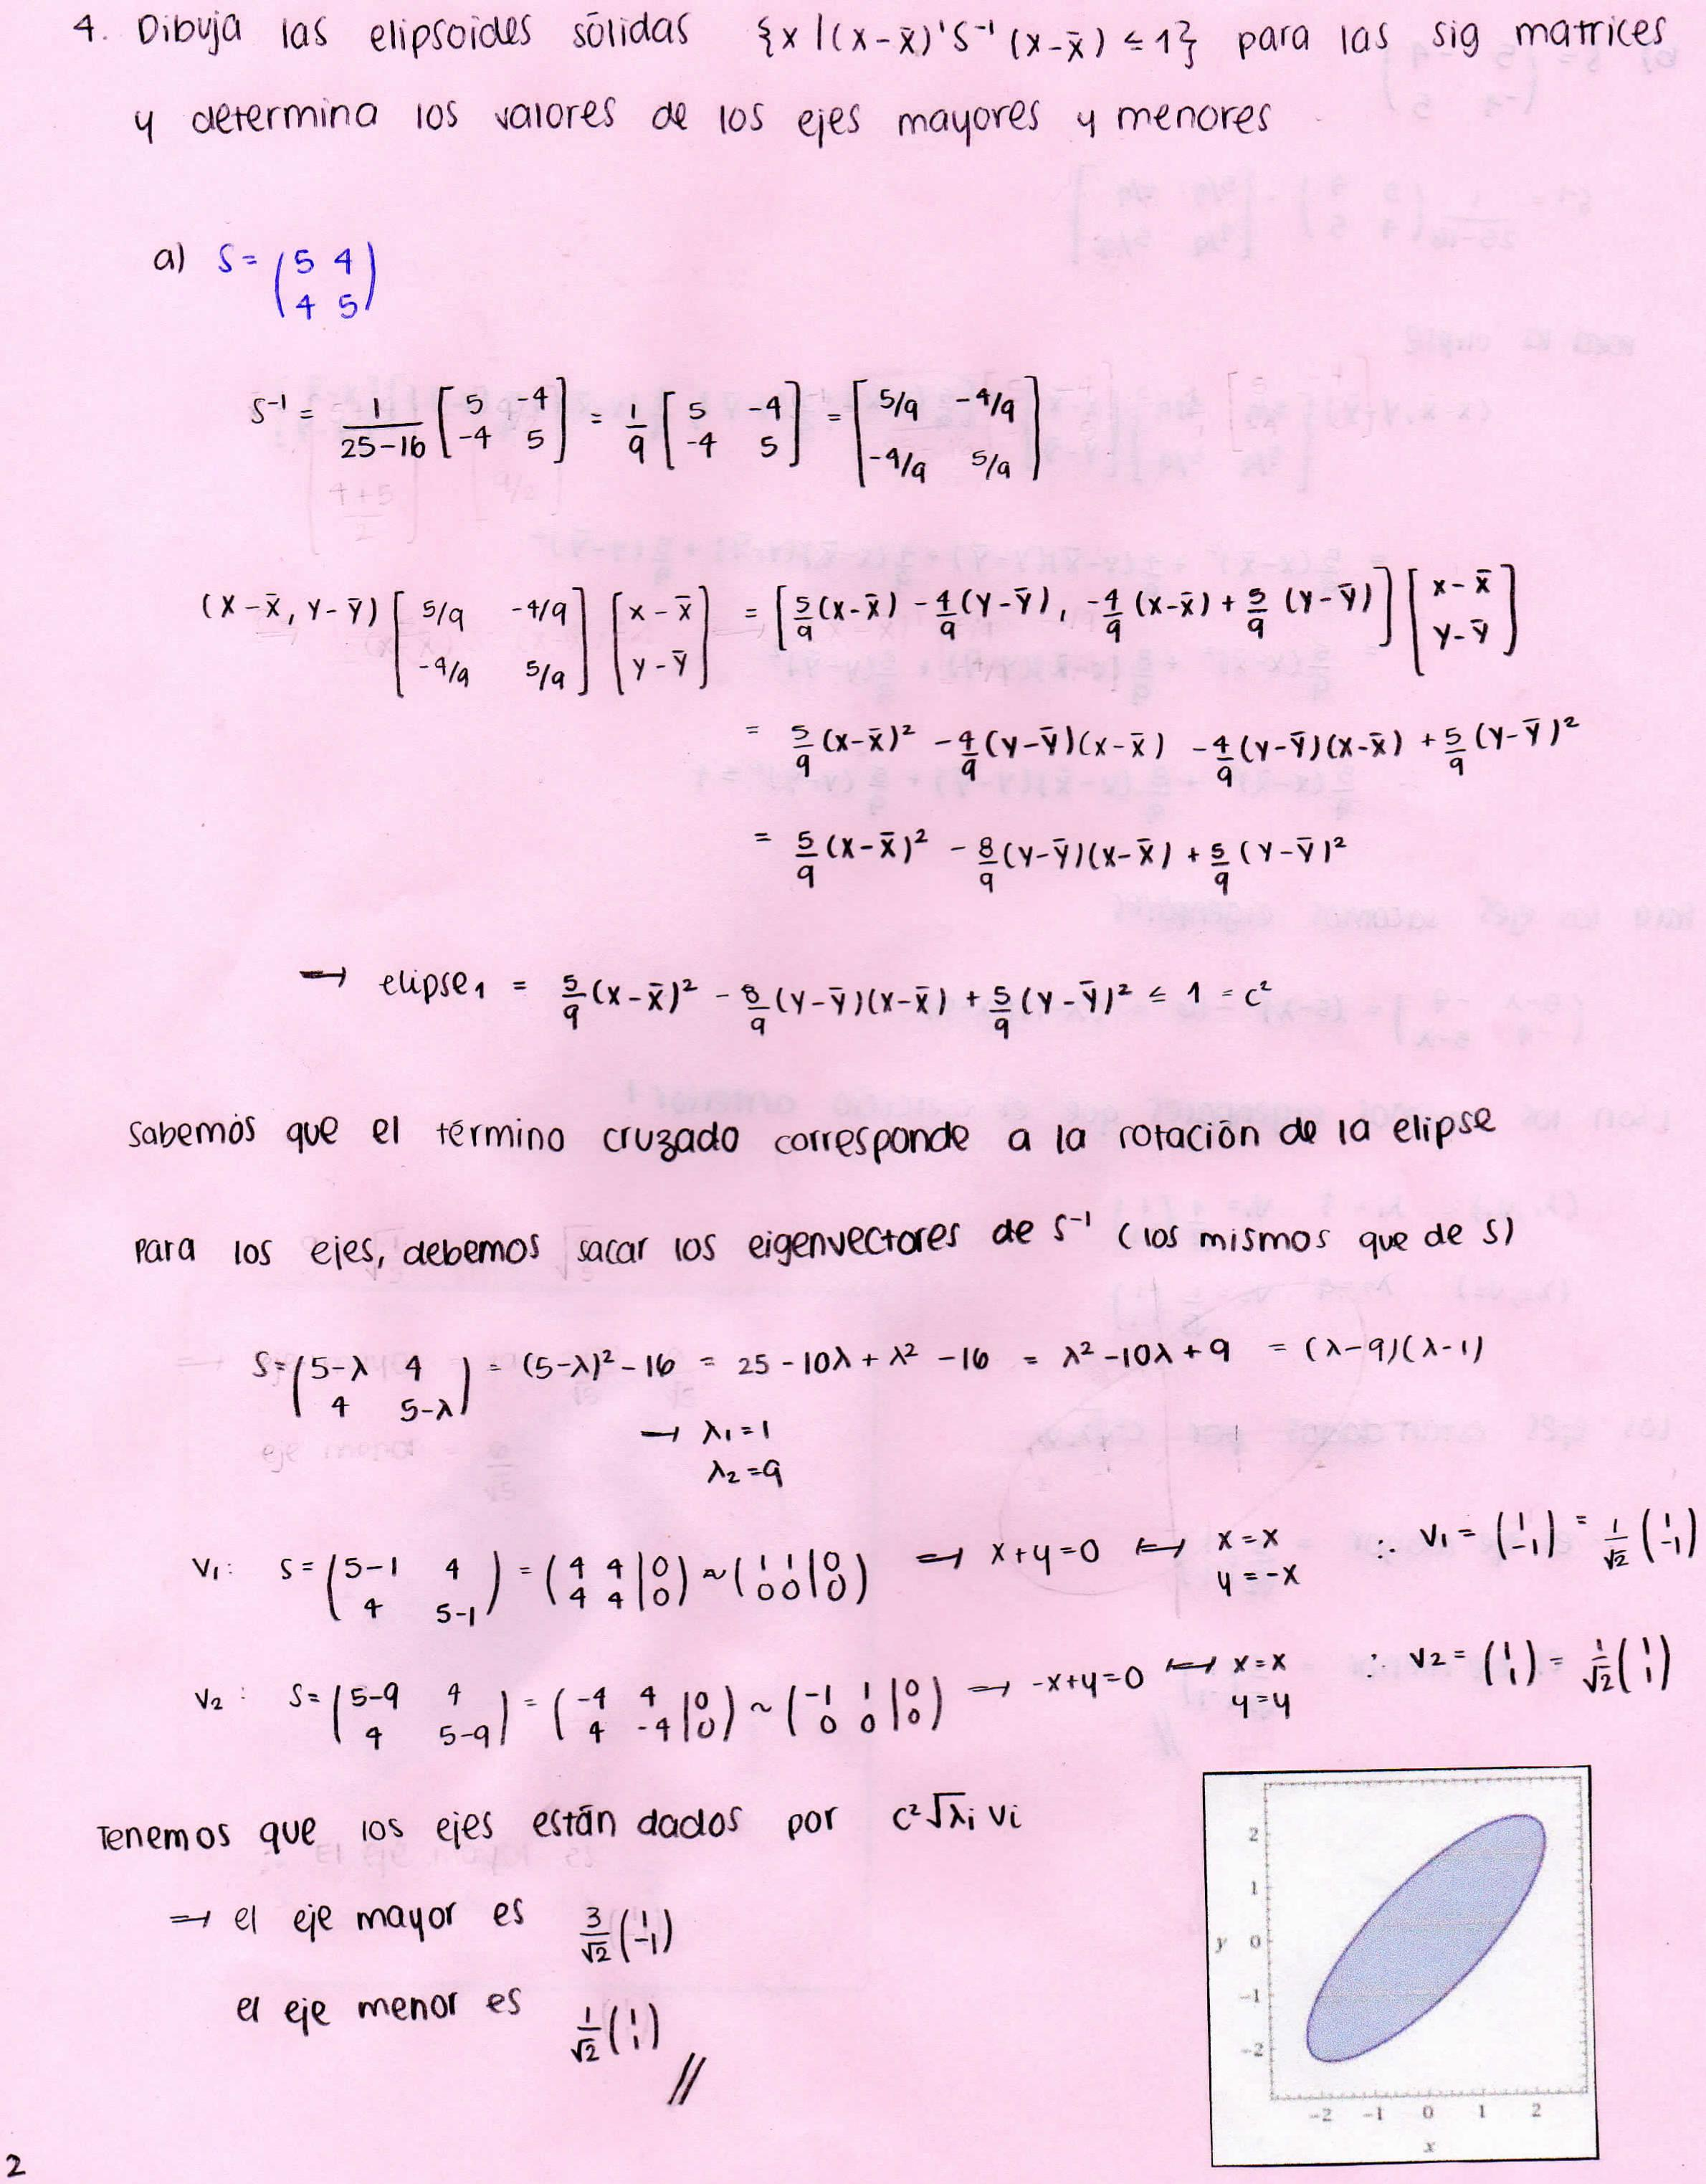
\includegraphics{4a.jpg}

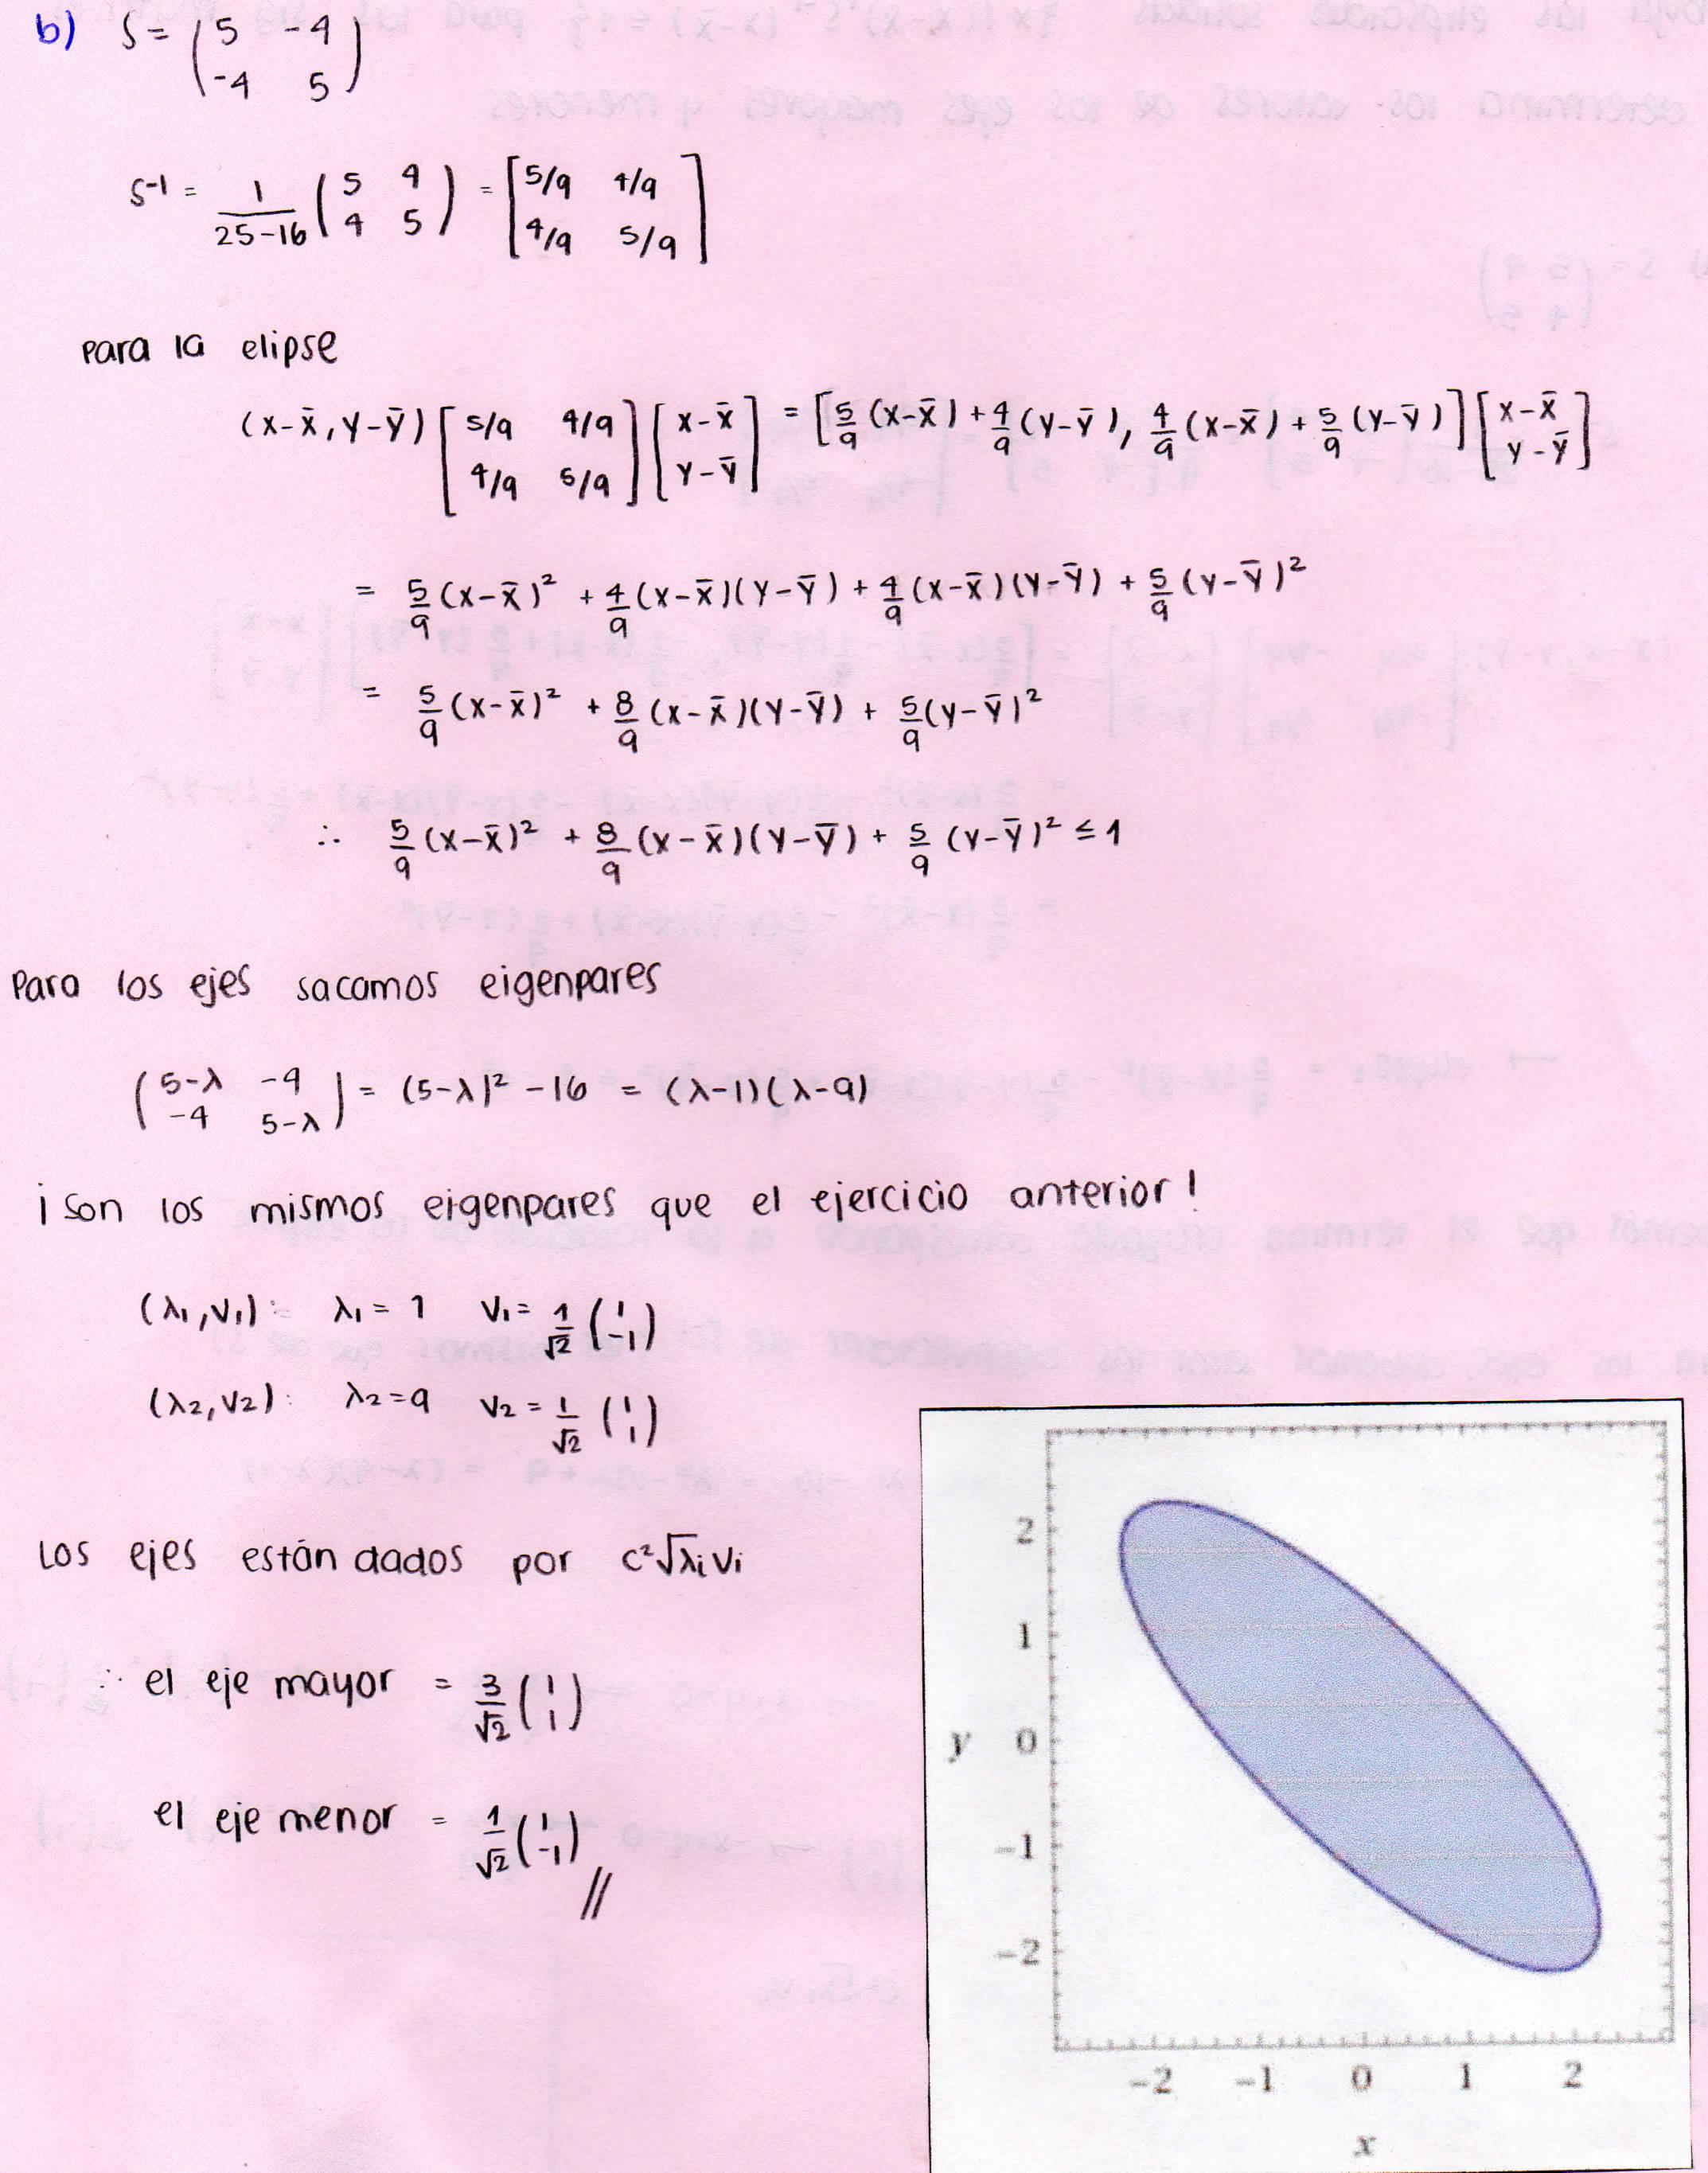
\includegraphics{4b.jpg}

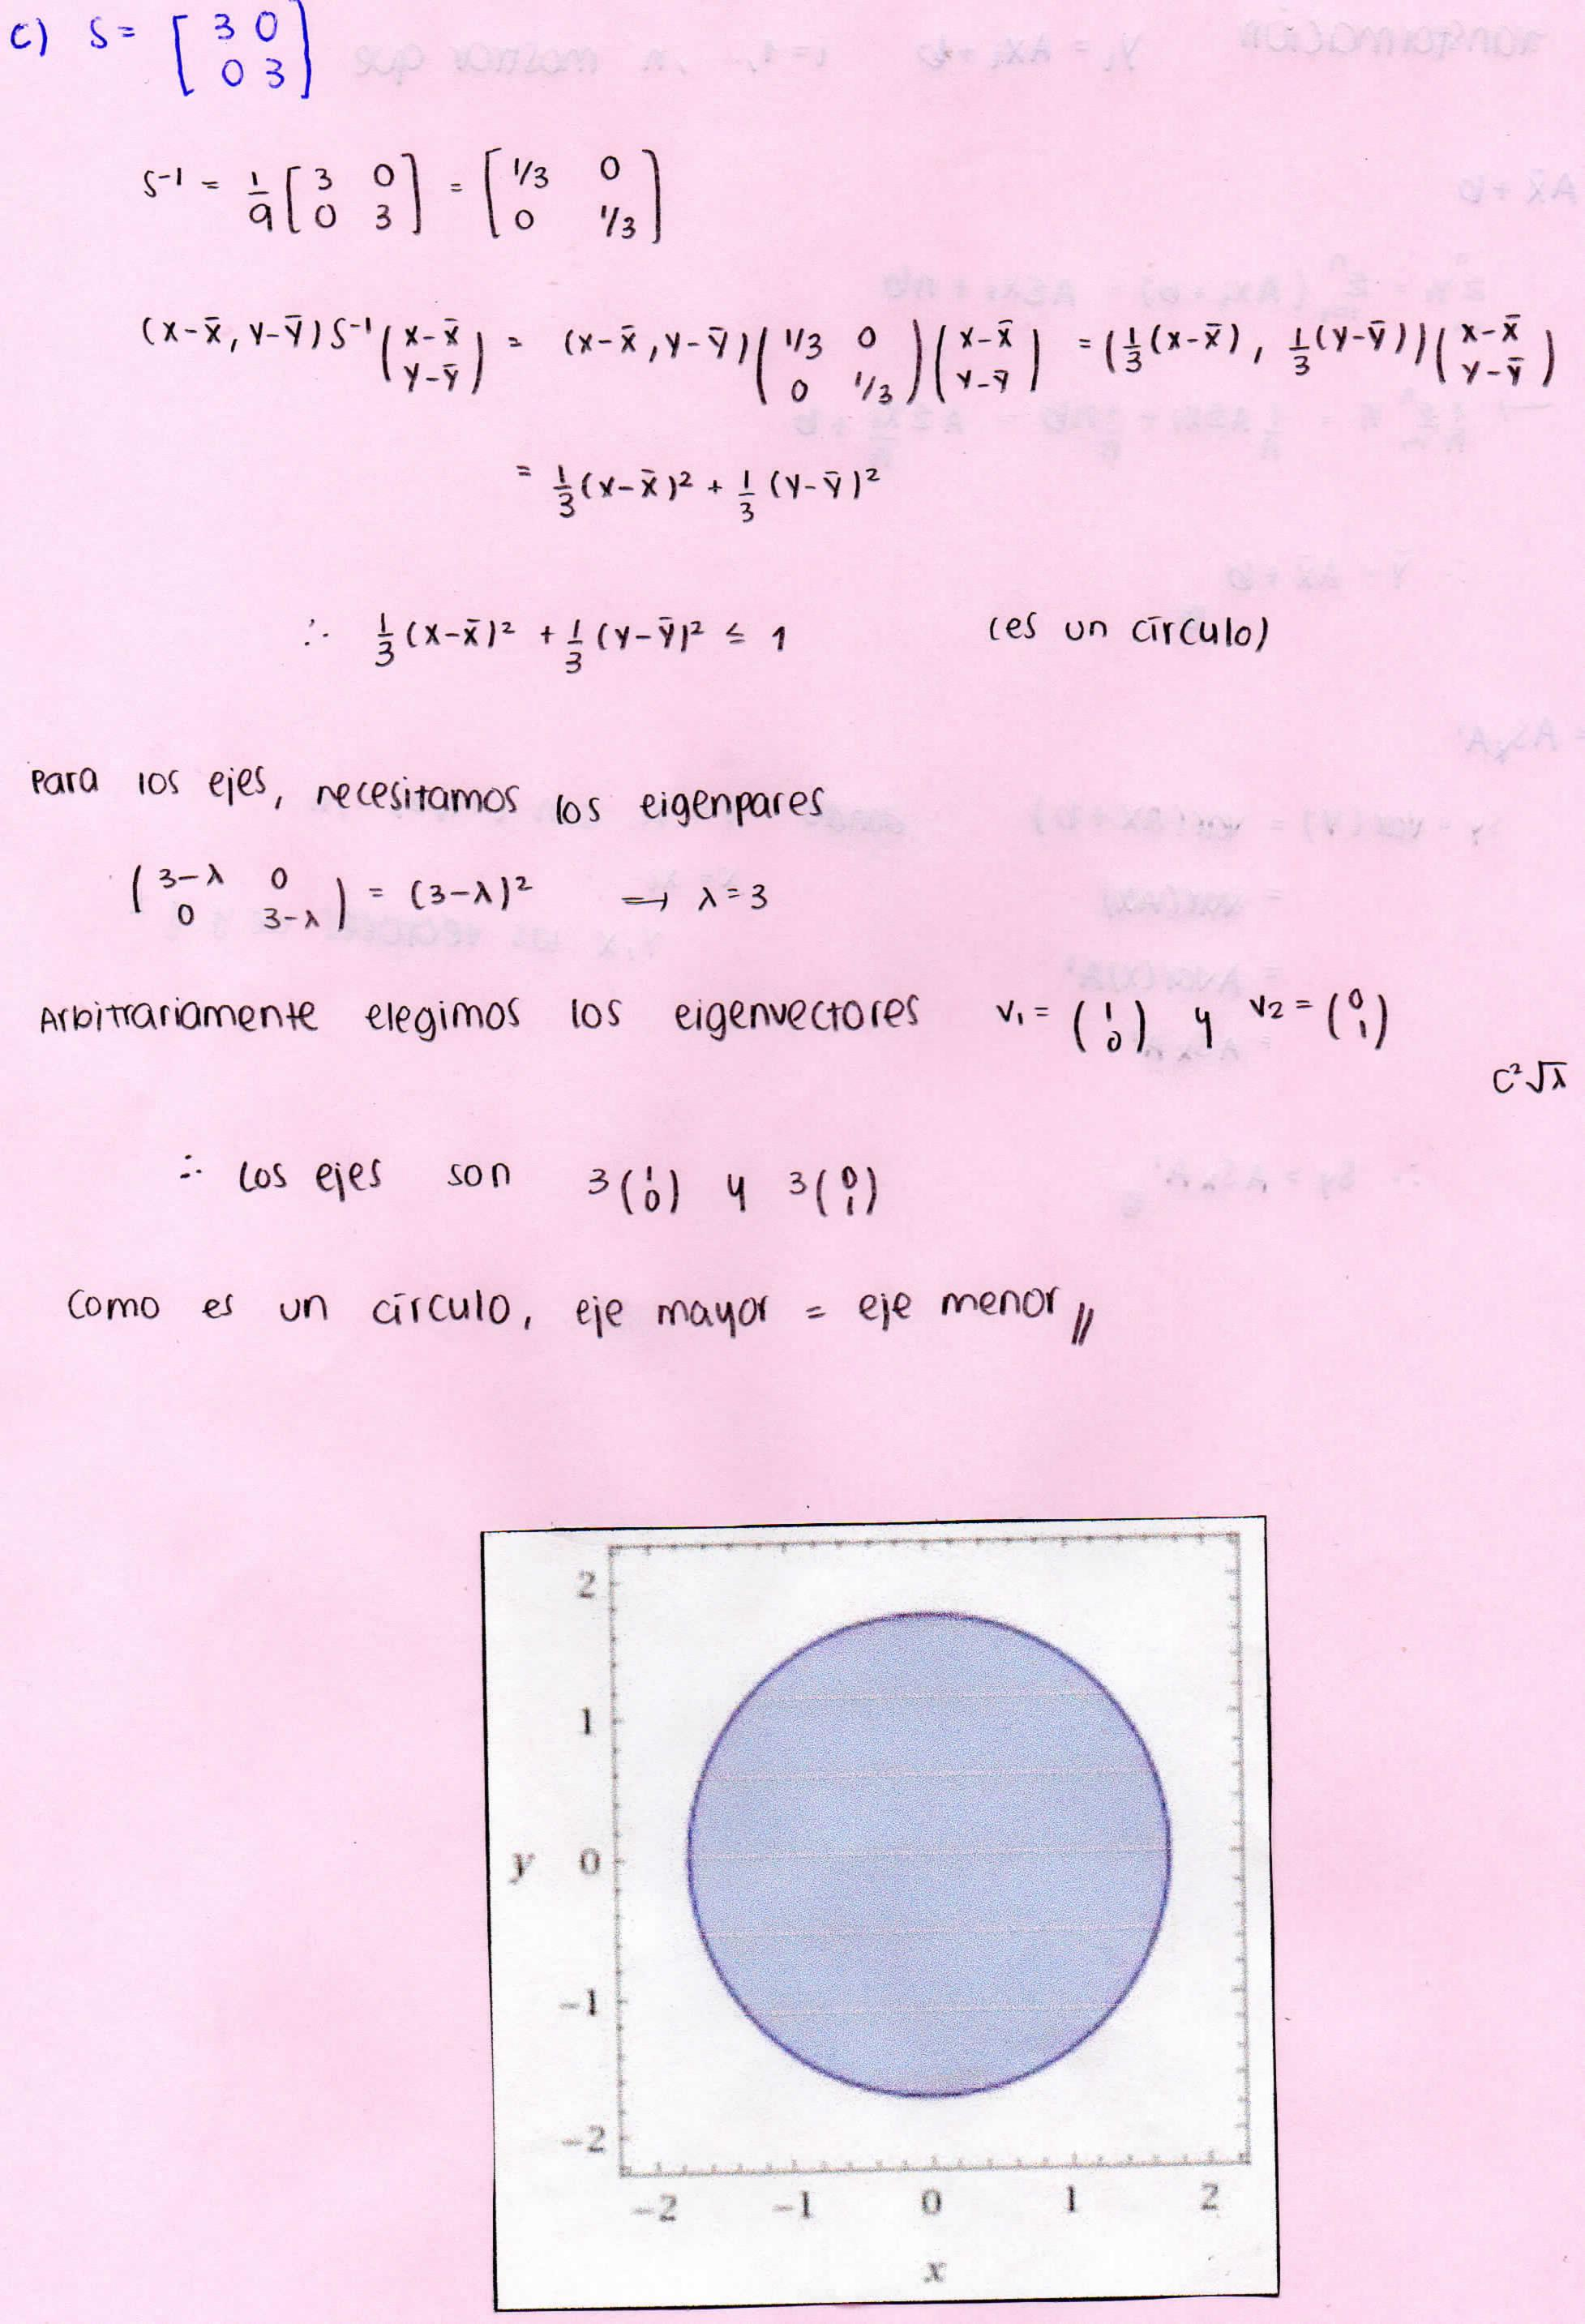
\includegraphics{4c.jpg}

\textbf{5. Archivo del INEGI}

\textbf{a. Configura la matriz X para poder operar con ella}

\begin{Shaded}
\begin{Highlighting}[]
\CommentTok{# datos <- read.csv("D:\textbackslash{}\textbackslash{}ITAM\textbackslash{}\textbackslash{}Aplicada III\textbackslash{}\textbackslash{}Tareas\textbackslash{}\textbackslash{}HW2\textbackslash{}\textbackslash{}INEGIConstruccion2017.csv", header=FALSE)}
\NormalTok{datos <-}\StringTok{ }\KeywordTok{read.csv}\NormalTok{(}\StringTok{".}\CharTok{\textbackslash{}\textbackslash{}}\StringTok{INEGIConstruccion2017.csv"}\NormalTok{, }\DataTypeTok{header=}\OtherTok{FALSE}\NormalTok{)}
\NormalTok{datos <-}\StringTok{ }\NormalTok{datos[}\OperatorTok{-}\DecValTok{1}\NormalTok{,]}

\KeywordTok{names}\NormalTok{(datos) <-}\StringTok{ }\KeywordTok{as.matrix}\NormalTok{(datos[}\DecValTok{1}\NormalTok{,])    }\CommentTok{# Tomo primer renglón}
\NormalTok{datos <-}\StringTok{ }\NormalTok{datos[}\OperatorTok{-}\DecValTok{1}\NormalTok{,]                     }\CommentTok{# Elimino el primer renglón}
\NormalTok{datos[] <-}\StringTok{ }\KeywordTok{lapply}\NormalTok{(datos, }\ControlFlowTok{function}\NormalTok{(x) }\KeywordTok{type.convert}\NormalTok{(}\KeywordTok{as.character}\NormalTok{(x))) }\CommentTok{# Primera columna names(datos) se vuelve el header}

\CommentTok{# Datos de enero 2017}
\NormalTok{datos <-}\StringTok{ }\NormalTok{datos }\OperatorTok\StringTok{ }\KeywordTok{filter}\NormalTok{(Periodo }\OperatorTok{==}\StringTok{ "2017/01"}\NormalTok{)}
\KeywordTok{head}\NormalTok{(datos)}
\end{Highlighting}
\end{Shaded}

\begin{verbatim}
##   Periodo
## 1 2017/01
##   Construcción (encuesta mensual) > Por entidad federativa > Horas trabajadas > Total Aguascalientes(Miles de horas) 
## 1                                                                                                            1441.083
##   Construcción (encuesta mensual) > Por entidad federativa > Horas trabajadas > Total Baja California(Miles de horas) 
## 1                                                                                                             3195.071
##   Construcción (encuesta mensual) > Por entidad federativa > Horas trabajadas > Total Baja California Sur(Miles de horas) 
## 1                                                                                                                  636.888
##   Construcción (encuesta mensual) > Por entidad federativa > Horas trabajadas > Total Campeche(Miles de horas) 
## 1                                                                                                      1669.002
##   Construcción (encuesta mensual) > Por entidad federativa > Horas trabajadas > Total Coahuila de Zaragoza(Miles de horas) 
## 1                                                                                                                  6140.209
##   Construcción (encuesta mensual) > Por entidad federativa > Horas trabajadas > Total Colima(Miles de horas) 
## 1                                                                                                    2189.691
##   Construcción (encuesta mensual) > Por entidad federativa > Horas trabajadas > Total Chiapas(Miles de horas) 
## 1                                                                                                     1469.275
##   Construcción (encuesta mensual) > Por entidad federativa > Horas trabajadas > Total Chihuahua(Miles de horas) 
## 1                                                                                                       7164.411
##   Construcción (encuesta mensual) > Por entidad federativa > Horas trabajadas > Total Ciudad de México(Miles de horas) 
## 1                                                                                                              15689.43
##   Construcción (encuesta mensual) > Por entidad federativa > Horas trabajadas > Total Durango(Miles de horas) 
## 1                                                                                                     4352.566
##   Construcción (encuesta mensual) > Por entidad federativa > Horas trabajadas > Total Guanajuato(Miles de horas) 
## 1                                                                                                        5636.278
##   Construcción (encuesta mensual) > Por entidad federativa > Horas trabajadas > Total Guerrero(Miles de horas) 
## 1                                                                                                      1511.229
##   Construcción (encuesta mensual) > Por entidad federativa > Horas trabajadas > Total Hidalgo(Miles de horas) 
## 1                                                                                                     1152.703
##   Construcción (encuesta mensual) > Por entidad federativa > Horas trabajadas > Total Jalisco(Miles de horas) 
## 1                                                                                                      8089.72
##   Construcción (encuesta mensual) > Por entidad federativa > Horas trabajadas > Total México(Miles de horas) 
## 1                                                                                                    5392.139
##   Construcción (encuesta mensual) > Por entidad federativa > Horas trabajadas > Total Michoacán de Ocampo(Miles de horas) 
## 1                                                                                                                 4084.203
##   Construcción (encuesta mensual) > Por entidad federativa > Horas trabajadas > Total Morelos(Miles de horas) 
## 1                                                                                                      550.092
##   Construcción (encuesta mensual) > Por entidad federativa > Horas trabajadas > Total Nayarit(Miles de horas) 
## 1                                                                                                     1929.037
##   Construcción (encuesta mensual) > Por entidad federativa > Horas trabajadas > Total Nuevo León(Miles de horas) 
## 1                                                                                                        13389.72
##   Construcción (encuesta mensual) > Por entidad federativa > Horas trabajadas > Total Oaxaca(Miles de horas) 
## 1                                                                                                     918.198
##   Construcción (encuesta mensual) > Por entidad federativa > Horas trabajadas > Total Puebla(Miles de horas) 
## 1                                                                                                    4487.444
##   Construcción (encuesta mensual) > Por entidad federativa > Horas trabajadas > Total Querétaro(Miles de horas) 
## 1                                                                                                       4037.281
##   Construcción (encuesta mensual) > Por entidad federativa > Horas trabajadas > Total Quintana Roo(Miles de horas) 
## 1                                                                                                          1947.345
##   Construcción (encuesta mensual) > Por entidad federativa > Horas trabajadas > Total San Luis Potosí(Miles de horas) 
## 1                                                                                                             2556.367
##   Construcción (encuesta mensual) > Por entidad federativa > Horas trabajadas > Total Sinaloa(Miles de horas) 
## 1                                                                                                     3345.227
##   Construcción (encuesta mensual) > Por entidad federativa > Horas trabajadas > Total Sonora(Miles de horas) 
## 1                                                                                                    6262.502
##   Construcción (encuesta mensual) > Por entidad federativa > Horas trabajadas > Total Tabasco(Miles de horas) 
## 1                                                                                                     2261.705
##   Construcción (encuesta mensual) > Por entidad federativa > Horas trabajadas > Total Tamaulipas(Miles de horas) 
## 1                                                                                                        6176.806
##   Construcción (encuesta mensual) > Por entidad federativa > Horas trabajadas > Total Tlaxcala(Miles de horas) 
## 1                                                                                                       268.718
##   Construcción (encuesta mensual) > Por entidad federativa > Horas trabajadas > Total Veracruz de Ignacio de la Llave(Miles de horas) 
## 1                                                                                                                             6582.393
##   Construcción (encuesta mensual) > Por entidad federativa > Horas trabajadas > Total Yucatán(Miles de horas) 
## 1                                                                                                     3423.691
##   Construcción (encuesta mensual) > Por entidad federativa > Horas trabajadas > Total Zacatecas(Miles de horas) 
## 1                                                                                                       1510.317
##   Construcción (encuesta mensual) > Por entidad federativa > Valor de producción generado en la entidad > En términos reales > Por tipo de obra > Total Total nacional(Miles de pesos a precios de junio de 2012.) 
## 1                                                                                                                                                                                                          33007657
##   Construcción (encuesta mensual) > Por entidad federativa > Valor de producción generado en la entidad > En términos reales > Por tipo de obra > Total Aguascalientes(Miles de pesos a precios de junio de 2012.) 
## 1                                                                                                                                                                                                          725965.1
##   Construcción (encuesta mensual) > Por entidad federativa > Valor de producción generado en la entidad > En términos reales > Por tipo de obra > Total Baja California(Miles de pesos a precios de junio de 2012.) 
## 1                                                                                                                                                                                                           872017.8
##   Construcción (encuesta mensual) > Por entidad federativa > Valor de producción generado en la entidad > En términos reales > Por tipo de obra > Total Baja California Sur(Miles de pesos a precios de junio de 2012.) 
## 1                                                                                                                                                                                                               438205.6
##   Construcción (encuesta mensual) > Por entidad federativa > Valor de producción generado en la entidad > En términos reales > Por tipo de obra > Total Campeche(Miles de pesos a precios de junio de 2012.) 
## 1                                                                                                                                                                                                    533582.3
##   Construcción (encuesta mensual) > Por entidad federativa > Valor de producción generado en la entidad > En términos reales > Por tipo de obra > Total Coahuila de Zaragoza(Miles de pesos a precios de junio de 2012.) 
## 1                                                                                                                                                                                                                 1059265
##   Construcción (encuesta mensual) > Por entidad federativa > Valor de producción generado en la entidad > En términos reales > Por tipo de obra > Total Colima(Miles de pesos a precios de junio de 2012.) 
## 1                                                                                                                                                                                                  414247.1
##   Construcción (encuesta mensual) > Por entidad federativa > Valor de producción generado en la entidad > En términos reales > Por tipo de obra > Total Chiapas(Miles de pesos a precios de junio de 2012.) 
## 1                                                                                                                                                                                                   717169.8
##   Construcción (encuesta mensual) > Por entidad federativa > Valor de producción generado en la entidad > En términos reales > Por tipo de obra > Total Chihuahua(Miles de pesos a precios de junio de 2012.) 
## 1                                                                                                                                                                                                      1404807
##   Construcción (encuesta mensual) > Por entidad federativa > Valor de producción generado en la entidad > En términos reales > Por tipo de obra > Total Ciudad de México(Miles de pesos a precios de junio de 2012.) 
## 1                                                                                                                                                                                                             2232550
##   Construcción (encuesta mensual) > Por entidad federativa > Valor de producción generado en la entidad > En términos reales > Por tipo de obra > Total Durango(Miles de pesos a precios de junio de 2012.) 
## 1                                                                                                                                                                                                     599605
##   Construcción (encuesta mensual) > Por entidad federativa > Valor de producción generado en la entidad > En términos reales > Por tipo de obra > Total Guanajuato(Miles de pesos a precios de junio de 2012.) 
## 1                                                                                                                                                                                                       2559232
##   Construcción (encuesta mensual) > Por entidad federativa > Valor de producción generado en la entidad > En términos reales > Por tipo de obra > Total Guerrero(Miles de pesos a precios de junio de 2012.) 
## 1                                                                                                                                                                                                    345778.8
##   Construcción (encuesta mensual) > Por entidad federativa > Valor de producción generado en la entidad > En términos reales > Por tipo de obra > Total Hidalgo(Miles de pesos a precios de junio de 2012.) 
## 1                                                                                                                                                                                                     539917
##   Construcción (encuesta mensual) > Por entidad federativa > Valor de producción generado en la entidad > En términos reales > Por tipo de obra > Total Jalisco(Miles de pesos a precios de junio de 2012.) 
## 1                                                                                                                                                                                                    2136522
##   Construcción (encuesta mensual) > Por entidad federativa > Valor de producción generado en la entidad > En términos reales > Por tipo de obra > Total México(Miles de pesos a precios de junio de 2012.) 
## 1                                                                                                                                                                                                   3144479
##   Construcción (encuesta mensual) > Por entidad federativa > Valor de producción generado en la entidad > En términos reales > Por tipo de obra > Total Michoacán de Ocampo(Miles de pesos a precios de junio de 2012.) 
## 1                                                                                                                                                                                                               558029.3
##   Construcción (encuesta mensual) > Por entidad federativa > Horas trabajadas > Dependiente > Total Total nacional(Miles de horas) 
## 1                                                                                                                          107742.6
##   Construcción (encuesta mensual) > Por entidad federativa > Horas trabajadas > Dependiente > Total Aguascalientes(Miles de horas) 
## 1                                                                                                                           1353.47
##   Construcción (encuesta mensual) > Por entidad federativa > Horas trabajadas > Dependiente > Total Baja California(Miles de horas) 
## 1                                                                                                                           2784.064
##   Construcción (encuesta mensual) > Por entidad federativa > Horas trabajadas > Dependiente > Total Baja California Sur(Miles de horas) 
## 1                                                                                                                                564.851
##   Construcción (encuesta mensual) > Por entidad federativa > Horas trabajadas > Dependiente > Total Campeche(Miles de horas) 
## 1                                                                                                                    1323.013
##   Construcción (encuesta mensual) > Por entidad federativa > Horas trabajadas > Dependiente > Total Coahuila de Zaragoza(Miles de horas) 
## 1                                                                                                                                4001.635
##   Construcción (encuesta mensual) > Por entidad federativa > Horas trabajadas > Dependiente > Total Colima(Miles de horas) 
## 1                                                                                                                  2152.042
##   Construcción (encuesta mensual) > Por entidad federativa > Horas trabajadas > Dependiente > Total Chiapas(Miles de horas) 
## 1                                                                                                                   1422.475
##   Construcción (encuesta mensual) > Por entidad federativa > Horas trabajadas > Dependiente > Total Chihuahua(Miles de horas) 
## 1                                                                                                                     6870.834
##   Construcción (encuesta mensual) > Por entidad federativa > Horas trabajadas > Dependiente > Total Ciudad de México(Miles de horas) 
## 1                                                                                                                            9407.633
##   Construcción (encuesta mensual) > Por entidad federativa > Horas trabajadas > Dependiente > Total Durango(Miles de horas) 
## 1                                                                                                                   4303.292
##   Construcción (encuesta mensual) > Por entidad federativa > Horas trabajadas > Dependiente > Total Guanajuato(Miles de horas) 
## 1                                                                                                                      5493.818
##   Construcción (encuesta mensual) > Por entidad federativa > Horas trabajadas > Dependiente > Total Guerrero(Miles de horas) 
## 1                                                                                                                    1435.678
##   Construcción (encuesta mensual) > Por entidad federativa > Horas trabajadas > Dependiente > Total Hidalgo(Miles de horas) 
## 1                                                                                                                   1146.944
##   Construcción (encuesta mensual) > Por entidad federativa > Horas trabajadas > Dependiente > Total Jalisco(Miles de horas) 
## 1                                                                                                                   7105.544
##   Construcción (encuesta mensual) > Por entidad federativa > Horas trabajadas > Dependiente > Total México(Miles de horas) 
## 1                                                                                                                  5045.081
##   Construcción (encuesta mensual) > Por entidad federativa > Horas trabajadas > Dependiente > Total Michoacán de Ocampo(Miles de horas) 
## 1                                                                                                                               3150.759
##   Construcción (encuesta mensual) > Por entidad federativa > Horas trabajadas > Dependiente > Total Morelos(Miles de horas) 
## 1                                                                                                                    511.352
##   Construcción (encuesta mensual) > Por entidad federativa > Horas trabajadas > Dependiente > Total Nayarit(Miles de horas) 
## 1                                                                                                                   1575.761
##   Construcción (encuesta mensual) > Por entidad federativa > Horas trabajadas > Dependiente > Total Nuevo León(Miles de horas) 
## 1                                                                                                                      8528.908
##   Construcción (encuesta mensual) > Por entidad federativa > Horas trabajadas > Dependiente > Total Oaxaca(Miles de horas) 
## 1                                                                                                                   881.406
##   Construcción (encuesta mensual) > Por entidad federativa > Horas trabajadas > Dependiente > Total Puebla(Miles de horas) 
## 1                                                                                                                   3833.66
##   Construcción (encuesta mensual) > Por entidad federativa > Horas trabajadas > Dependiente > Total Querétaro(Miles de horas) 
## 1                                                                                                                     3778.835
##   Construcción (encuesta mensual) > Por entidad federativa > Horas trabajadas > Dependiente > Total Quintana Roo(Miles de horas) 
## 1                                                                                                                        1765.056
##   Construcción (encuesta mensual) > Por entidad federativa > Horas trabajadas > Dependiente > Total San Luis Potosí(Miles de horas) 
## 1                                                                                                                           2365.318
##   Construcción (encuesta mensual) > Por entidad federativa > Horas trabajadas > Dependiente > Total Sinaloa(Miles de horas) 
## 1                                                                                                                   3143.382
##   Construcción (encuesta mensual) > Por entidad federativa > Horas trabajadas > Dependiente > Total Sonora(Miles de horas) 
## 1                                                                                                                  5555.881
##   Construcción (encuesta mensual) > Por entidad federativa > Horas trabajadas > Dependiente > Total Tabasco(Miles de horas) 
## 1                                                                                                                   1716.063
##   Construcción (encuesta mensual) > Por entidad federativa > Horas trabajadas > Dependiente > Total Tamaulipas(Miles de horas) 
## 1                                                                                                                      5224.554
##   Construcción (encuesta mensual) > Por entidad federativa > Horas trabajadas > Dependiente > Total Tlaxcala(Miles de horas) 
## 1                                                                                                                      268.21
##   Construcción (encuesta mensual) > Por entidad federativa > Horas trabajadas > Dependiente > Total Veracruz de Ignacio de la Llave(Miles de horas) 
## 1                                                                                                                                           6226.744
##   Construcción (encuesta mensual) > Por entidad federativa > Horas trabajadas > Dependiente > Total Yucatán(Miles de horas) 
## 1                                                                                                                   3310.421
##   Construcción (encuesta mensual) > Por entidad federativa > Horas trabajadas > Dependiente > Total Zacatecas(Miles de horas) 
## 1                                                                                                                     1495.929
##   Construcción (encuesta mensual) > Por entidad federativa > Horas trabajadas > Dependiente > Obreros Total nacional(Miles de horas) 
## 1                                                                                                                            84562.85
##   Construcción (encuesta mensual) > Por entidad federativa > Horas trabajadas > Dependiente > Obreros Aguascalientes(Miles de horas) 
## 1                                                                                                                            1055.779
##   Construcción (encuesta mensual) > Por entidad federativa > Horas trabajadas > Dependiente > Obreros Baja California(Miles de horas) 
## 1                                                                                                                             2045.011
##   Construcción (encuesta mensual) > Por entidad federativa > Horas trabajadas > Dependiente > Obreros Baja California Sur(Miles de horas) 
## 1                                                                                                                                  329.325
##   Construcción (encuesta mensual) > Por entidad federativa > Horas trabajadas > Dependiente > Obreros Campeche(Miles de horas) 
## 1                                                                                                                        958.88
##   Construcción (encuesta mensual) > Por entidad federativa > Horas trabajadas > Dependiente > Obreros Coahuila de Zaragoza(Miles de horas) 
## 1                                                                                                                                  3304.095
##   Construcción (encuesta mensual) > Por entidad federativa > Horas trabajadas > Dependiente > Obreros Colima(Miles de horas) 
## 1                                                                                                                    1804.447
##   Construcción (encuesta mensual) > Por entidad federativa > Horas trabajadas > Dependiente > Obreros Chiapas(Miles de horas) 
## 1                                                                                                                      893.406
##   Construcción (encuesta mensual) > Por entidad federativa > Horas trabajadas > Dependiente > Obreros Chihuahua(Miles de horas) 
## 1                                                                                                                        5722.79
##   Construcción (encuesta mensual) > Por entidad federativa > Horas trabajadas > Dependiente > Obreros Ciudad de México(Miles de horas) 
## 1                                                                                                                              6836.521
##   Construcción (encuesta mensual) > Por entidad federativa > Horas trabajadas > Dependiente > Obreros Durango(Miles de horas) 
## 1                                                                                                                     3874.623
##   Construcción (encuesta mensual) > Por entidad federativa > Horas trabajadas > Dependiente > Obreros Guanajuato(Miles de horas) 
## 1                                                                                                                        4412.815
##   Construcción (encuesta mensual) > Por entidad federativa > Horas trabajadas > Dependiente > Obreros Guerrero(Miles de horas) 
## 1                                                                                                                      1166.891
##   Construcción (encuesta mensual) > Por entidad federativa > Horas trabajadas > Dependiente > Obreros Hidalgo(Miles de horas) 
## 1                                                                                                                      882.737
##   Construcción (encuesta mensual) > Por entidad federativa > Horas trabajadas > Dependiente > Obreros Jalisco(Miles de horas) 
## 1                                                                                                                     5830.045
##   Construcción (encuesta mensual) > Por entidad federativa > Horas trabajadas > Dependiente > Obreros México(Miles de horas) 
## 1                                                                                                                    3118.509
##   Construcción (encuesta mensual) > Por entidad federativa > Horas trabajadas > Dependiente > Obreros Michoacán de Ocampo(Miles de horas) 
## 1                                                                                                                                 2363.378
##   Construcción (encuesta mensual) > Por entidad federativa > Horas trabajadas > Dependiente > Obreros Morelos(Miles de horas) 
## 1                                                                                                                      356.827
##   Construcción (encuesta mensual) > Por entidad federativa > Horas trabajadas > Dependiente > Obreros Nayarit(Miles de horas) 
## 1                                                                                                                     1273.005
##   Construcción (encuesta mensual) > Por entidad federativa > Horas trabajadas > Dependiente > Obreros Nuevo León(Miles de horas) 
## 1                                                                                                                        6926.857
##   Construcción (encuesta mensual) > Por entidad federativa > Horas trabajadas > Dependiente > Obreros Oaxaca(Miles de horas) 
## 1                                                                                                                     549.736
##   Construcción (encuesta mensual) > Por entidad federativa > Horas trabajadas > Dependiente > Obreros Puebla(Miles de horas) 
## 1                                                                                                                    3122.048
##   Construcción (encuesta mensual) > Por entidad federativa > Horas trabajadas > Dependiente > Obreros Querétaro(Miles de horas) 
## 1                                                                                                                       3173.833
##   Construcción (encuesta mensual) > Por entidad federativa > Horas trabajadas > Dependiente > Obreros Quintana Roo(Miles de horas) 
## 1                                                                                                                          1395.071
##   Construcción (encuesta mensual) > Por entidad federativa > Horas trabajadas > Dependiente > Obreros San Luis Potosí(Miles de horas) 
## 1                                                                                                                             1799.165
##   Construcción (encuesta mensual) > Por entidad federativa > Horas trabajadas > Dependiente > Obreros Sinaloa(Miles de horas) 
## 1                                                                                                                     2267.931
##   Construcción (encuesta mensual) > Por entidad federativa > Horas trabajadas > Dependiente > Obreros Sonora(Miles de horas) 
## 1                                                                                                                    4631.798
##   Construcción (encuesta mensual) > Por entidad federativa > Horas trabajadas > Dependiente > Obreros Tabasco(Miles de horas) 
## 1                                                                                                                     1169.822
##   Construcción (encuesta mensual) > Por entidad federativa > Horas trabajadas > Dependiente > Obreros Tamaulipas(Miles de horas) 
## 1                                                                                                                        4208.895
##   Construcción (encuesta mensual) > Por entidad federativa > Horas trabajadas > Dependiente > Obreros Tlaxcala(Miles de horas) 
## 1                                                                                                                       200.665
##   Construcción (encuesta mensual) > Por entidad federativa > Horas trabajadas > Dependiente > Obreros Veracruz de Ignacio de la Llave(Miles de horas) 
## 1                                                                                                                                             5041.573
##   Construcción (encuesta mensual) > Por entidad federativa > Horas trabajadas > Dependiente > Obreros Yucatán(Miles de horas) 
## 1                                                                                                                     2572.381
##   Construcción (encuesta mensual) > Por entidad federativa > Horas trabajadas > Dependiente > Obreros Zacatecas(Miles de horas) 
## 1                                                                                                                       1273.993
##   Construcción (encuesta mensual) > Por entidad federativa > Horas trabajadas > Dependiente > Empleados Total nacional(Miles de horas) 
## 1                                                                                                                              21536.76
##   Construcción (encuesta mensual) > Por entidad federativa > Horas trabajadas > Dependiente > Empleados Aguascalientes(Miles de horas) 
## 1                                                                                                                               268.036
##   Construcción (encuesta mensual) > Por entidad federativa > Horas trabajadas > Dependiente > Empleados Baja California(Miles de horas) 
## 1                                                                                                                                723.914
##   Construcción (encuesta mensual) > Por entidad federativa > Horas trabajadas > Dependiente > Empleados Baja California Sur(Miles de horas) 
## 1                                                                                                                                    200.202
##   Construcción (encuesta mensual) > Por entidad federativa > Horas trabajadas > Dependiente > Empleados Campeche(Miles de horas) 
## 1                                                                                                                         349.655
##   Construcción (encuesta mensual) > Por entidad federativa > Horas trabajadas > Dependiente > Empleados Coahuila de Zaragoza(Miles de horas) 
## 1                                                                                                                                     619.639
##   Construcción (encuesta mensual) > Por entidad federativa > Horas trabajadas > Dependiente > Empleados Colima(Miles de horas) 
## 1                                                                                                                       320.512
##   Construcción (encuesta mensual) > Por entidad federativa > Horas trabajadas > Dependiente > Empleados Chiapas(Miles de horas) 
## 1                                                                                                                        492.414
##   Construcción (encuesta mensual) > Por entidad federativa > Horas trabajadas > Dependiente > Empleados Chihuahua(Miles de horas) 
## 1                                                                                                                         1079.958
##   Construcción (encuesta mensual) > Por entidad federativa > Horas trabajadas > Dependiente > Empleados Ciudad de México(Miles de horas) 
## 1                                                                                                                                2430.036
##   Construcción (encuesta mensual) > Por entidad federativa > Horas trabajadas > Dependiente > Empleados Durango(Miles de horas) 
## 1                                                                                                                        407.282
##   Construcción (encuesta mensual) > Por entidad federativa > Horas trabajadas > Dependiente > Empleados Guanajuato(Miles de horas) 
## 1                                                                                                                           962.888
##   Construcción (encuesta mensual) > Por entidad federativa > Horas trabajadas > Dependiente > Empleados Guerrero(Miles de horas) 
## 1                                                                                                                         236.075
##   Construcción (encuesta mensual) > Por entidad federativa > Horas trabajadas > Dependiente > Empleados Hidalgo(Miles de horas) 
## 1                                                                                                                        225.714
##   Construcción (encuesta mensual) > Por entidad federativa > Horas trabajadas > Dependiente > Empleados Jalisco(Miles de horas) 
## 1                                                                                                                       1188.357
##   Construcción (encuesta mensual) > Por entidad federativa > Horas trabajadas > Dependiente > Empleados México(Miles de horas) 
## 1                                                                                                                      1814.544
##   Construcción (encuesta mensual) > Por entidad federativa > Horas trabajadas > Dependiente > Empleados Michoacán de Ocampo(Miles de horas) 
## 1                                                                                                                                    715.655
##   Construcción (encuesta mensual) > Por entidad federativa > Horas trabajadas > Dependiente > Empleados Morelos(Miles de horas) 
## 1                                                                                                                        129.513
##   Construcción (encuesta mensual) > Por entidad federativa > Horas trabajadas > Dependiente > Empleados Nayarit(Miles de horas) 
## 1                                                                                                                        271.445
##   Construcción (encuesta mensual) > Por entidad federativa > Horas trabajadas > Dependiente > Empleados Nuevo León(Miles de horas) 
## 1                                                                                                                          1530.889
##   Construcción (encuesta mensual) > Por entidad federativa > Horas trabajadas > Dependiente > Empleados Oaxaca(Miles de horas) 
## 1                                                                                                                       249.908
##   Construcción (encuesta mensual) > Por entidad federativa > Horas trabajadas > Dependiente > Empleados Puebla(Miles de horas) 
## 1                                                                                                                       645.089
##   Construcción (encuesta mensual) > Por entidad federativa > Horas trabajadas > Dependiente > Empleados Querétaro(Miles de horas) 
## 1                                                                                                                          563.313
##   Construcción (encuesta mensual) > Por entidad federativa > Horas trabajadas > Dependiente > Empleados Quintana Roo(Miles de horas) 
## 1                                                                                                                             359.425
##   Construcción (encuesta mensual) > Por entidad federativa > Horas trabajadas > Dependiente > Empleados San Luis Potosí(Miles de horas) 
## 1                                                                                                                                511.367
##   Construcción (encuesta mensual) > Por entidad federativa > Horas trabajadas > Dependiente > Empleados Sinaloa(Miles de horas) 
## 1                                                                                                                        789.313
##   Construcción (encuesta mensual) > Por entidad federativa > Horas trabajadas > Dependiente > Empleados Sonora(Miles de horas) 
## 1                                                                                                                       911.309
##   Construcción (encuesta mensual) > Por entidad federativa > Horas trabajadas > Dependiente > Empleados Tabasco(Miles de horas) 
## 1                                                                                                                        501.094
##   Construcción (encuesta mensual) > Por entidad federativa > Horas trabajadas > Dependiente > Empleados Tamaulipas(Miles de horas) 
## 1                                                                                                                           950.857
##   Construcción (encuesta mensual) > Por entidad federativa > Horas trabajadas > Dependiente > Empleados Tlaxcala(Miles de horas) 
## 1                                                                                                                           57.04
##   Construcción (encuesta mensual) > Por entidad federativa > Horas trabajadas > Dependiente > Empleados Veracruz de Ignacio de la Llave(Miles de horas) 
## 1                                                                                                                                               1113.837
##   Construcción (encuesta mensual) > Por entidad federativa > Horas trabajadas > Dependiente > Empleados Yucatán(Miles de horas) 
## 1                                                                                                                         708.74
##   Construcción (encuesta mensual) > Por entidad federativa > Horas trabajadas > Dependiente > Empleados Zacatecas(Miles de horas) 
## 1                                                                                                                          208.743
##   Construcción (encuesta mensual) > Por entidad federativa > Horas trabajadas > Dependiente > Propietarios, familiares y otros trabajadores no remunerados Total nacional(Miles de horas) 
## 1                                                                                                                                                                                 1642.998
##   Construcción (encuesta mensual) > Por entidad federativa > Horas trabajadas > Dependiente > Propietarios, familiares y otros trabajadores no remunerados Aguascalientes(Miles de horas) 
## 1                                                                                                                                                                                   29.655
##   Construcción (encuesta mensual) > Por entidad federativa > Horas trabajadas > Dependiente > Propietarios, familiares y otros trabajadores no remunerados Baja California(Miles de horas) 
## 1                                                                                                                                                                                    15.139
##   Construcción (encuesta mensual) > Por entidad federativa > Horas trabajadas > Dependiente > Propietarios, familiares y otros trabajadores no remunerados Baja California Sur(Miles de horas) 
## 1                                                                                                                                                                                        35.324
##   Construcción (encuesta mensual) > Por entidad federativa > Horas trabajadas > Dependiente > Propietarios, familiares y otros trabajadores no remunerados Campeche(Miles de horas) 
## 1                                                                                                                                                                             14.478
##   Construcción (encuesta mensual) > Por entidad federativa > Horas trabajadas > Dependiente > Propietarios, familiares y otros trabajadores no remunerados Coahuila de Zaragoza(Miles de horas) 
## 1                                                                                                                                                                                         77.901
##   Construcción (encuesta mensual) > Por entidad federativa > Horas trabajadas > Dependiente > Propietarios, familiares y otros trabajadores no remunerados Colima(Miles de horas) 
## 1                                                                                                                                                                           27.083
##   Construcción (encuesta mensual) > Por entidad federativa > Horas trabajadas > Dependiente > Propietarios, familiares y otros trabajadores no remunerados Chiapas(Miles de horas) 
## 1                                                                                                                                                                            36.655
##   Construcción (encuesta mensual) > Por entidad federativa > Horas trabajadas > Dependiente > Propietarios, familiares y otros trabajadores no remunerados Chihuahua(Miles de horas) 
## 1                                                                                                                                                                              68.086
##   Construcción (encuesta mensual) > Por entidad federativa > Horas trabajadas > Dependiente > Propietarios, familiares y otros trabajadores no remunerados Ciudad de México(Miles de horas) 
## 1                                                                                                                                                                                    141.076
##   Construcción (encuesta mensual) > Por entidad federativa > Horas trabajadas > Dependiente > Propietarios, familiares y otros trabajadores no remunerados Durango(Miles de horas) 
## 1                                                                                                                                                                            21.387
##   Construcción (encuesta mensual) > Por entidad federativa > Horas trabajadas > Dependiente > Propietarios, familiares y otros trabajadores no remunerados Guanajuato(Miles de horas) 
## 1                                                                                                                                                                              118.115
##   Construcción (encuesta mensual) > Por entidad federativa > Horas trabajadas > Dependiente > Propietarios, familiares y otros trabajadores no remunerados Guerrero(Miles de horas) 
## 1                                                                                                                                                                             32.712
##   Construcción (encuesta mensual) > Por entidad federativa > Horas trabajadas > Dependiente > Propietarios, familiares y otros trabajadores no remunerados Hidalgo(Miles de horas) 
## 1                                                                                                                                                                            38.493
##   Construcción (encuesta mensual) > Por entidad federativa > Horas trabajadas > Dependiente > Propietarios, familiares y otros trabajadores no remunerados Jalisco(Miles de horas) 
## 1                                                                                                                                                                            87.142
##   Construcción (encuesta mensual) > Por entidad federativa > Horas trabajadas > Dependiente > Propietarios, familiares y otros trabajadores no remunerados México(Miles de horas) 
## 1                                                                                                                                                                          112.028
##   Construcción (encuesta mensual) > Por entidad federativa > Horas trabajadas > Dependiente > Propietarios, familiares y otros trabajadores no remunerados Michoacán de Ocampo(Miles de horas) 
## 1                                                                                                                                                                                        71.726
##   Construcción (encuesta mensual) > Por entidad federativa > Horas trabajadas > Dependiente > Propietarios, familiares y otros trabajadores no remunerados Morelos(Miles de horas) 
## 1                                                                                                                                                                            25.012
##   Construcción (encuesta mensual) > Por entidad federativa > Horas trabajadas > Dependiente > Propietarios, familiares y otros trabajadores no remunerados Nayarit(Miles de horas) 
## 1                                                                                                                                                                            31.311
##   Construcción (encuesta mensual) > Por entidad federativa > Horas trabajadas > Dependiente > Propietarios, familiares y otros trabajadores no remunerados Nuevo León(Miles de horas) 
## 1                                                                                                                                                                               71.162
##   Construcción (encuesta mensual) > Por entidad federativa > Horas trabajadas > Dependiente > Propietarios, familiares y otros trabajadores no remunerados Oaxaca(Miles de horas) 
## 1                                                                                                                                                                           81.762
##   Construcción (encuesta mensual) > Por entidad federativa > Horas trabajadas > Dependiente > Propietarios, familiares y otros trabajadores no remunerados Puebla(Miles de horas) 
## 1                                                                                                                                                                           66.523
##   Construcción (encuesta mensual) > Por entidad federativa > Horas trabajadas > Dependiente > Propietarios, familiares y otros trabajadores no remunerados Querétaro(Miles de horas) 
## 1                                                                                                                                                                              41.689
##   Construcción (encuesta mensual) > Por entidad federativa > Horas trabajadas > Dependiente > Propietarios, familiares y otros trabajadores no remunerados Quintana Roo(Miles de horas) 
## 1                                                                                                                                                                                  10.56
##   Construcción (encuesta mensual) > Por entidad federativa > Horas trabajadas > Dependiente > Propietarios, familiares y otros trabajadores no remunerados San Luis Potosí(Miles de horas) 
## 1                                                                                                                                                                                    54.786
##   Construcción (encuesta mensual) > Por entidad federativa > Horas trabajadas > Dependiente > Propietarios, familiares y otros trabajadores no remunerados Sinaloa(Miles de horas) 
## 1                                                                                                                                                                            86.138
##   Construcción (encuesta mensual) > Por entidad federativa > Horas trabajadas > Dependiente > Propietarios, familiares y otros trabajadores no remunerados Sonora(Miles de horas) 
## 1                                                                                                                                                                           12.774
##   Construcción (encuesta mensual) > Por entidad federativa > Horas trabajadas > Dependiente > Propietarios, familiares y otros trabajadores no remunerados Tabasco(Miles de horas) 
## 1                                                                                                                                                                            45.147
##   Construcción (encuesta mensual) > Por entidad federativa > Horas trabajadas > Dependiente > Propietarios, familiares y otros trabajadores no remunerados Tamaulipas(Miles de horas) 
## 1                                                                                                                                                                               64.802
##   Construcción (encuesta mensual) > Por entidad federativa > Horas trabajadas > Dependiente > Propietarios, familiares y otros trabajadores no remunerados Tlaxcala(Miles de horas) 
## 1                                                                                                                                                                             10.505
##   Construcción (encuesta mensual) > Por entidad federativa > Horas trabajadas > Dependiente > Propietarios, familiares y otros trabajadores no remunerados Veracruz de Ignacio de la Llave(Miles de horas) 
## 1                                                                                                                                                                                                    71.334
##   Construcción (encuesta mensual) > Por entidad federativa > Horas trabajadas > Dependiente > Propietarios, familiares y otros trabajadores no remunerados Yucatán(Miles de horas) 
## 1                                                                                                                                                                              29.3
##   Construcción (encuesta mensual) > Por entidad federativa > Horas trabajadas > Dependiente > Propietarios, familiares y otros trabajadores no remunerados Zacatecas(Miles de horas) 
## 1                                                                                                                                                                              13.193
##   Construcción (encuesta mensual) > Por entidad federativa > Horas trabajadas > No dependiente Total nacional(Miles de horas) 
## 1                                                                                                                     21718.14
##   Construcción (encuesta mensual) > Por entidad federativa > Horas trabajadas > No dependiente Aguascalientes(Miles de horas) 
## 1                                                                                                                       87.613
##   Construcción (encuesta mensual) > Por entidad federativa > Horas trabajadas > No dependiente Baja California(Miles de horas) 
## 1                                                                                                                       411.007
##   Construcción (encuesta mensual) > Por entidad federativa > Horas trabajadas > No dependiente Baja California Sur(Miles de horas) 
## 1                                                                                                                            72.037
##   Construcción (encuesta mensual) > Por entidad federativa > Horas trabajadas > No dependiente Campeche(Miles de horas) 
## 1                                                                                                                345.989
##   Construcción (encuesta mensual) > Por entidad federativa > Horas trabajadas > No dependiente Coahuila de Zaragoza(Miles de horas) 
## 1                                                                                                                           2138.574
##   Construcción (encuesta mensual) > Por entidad federativa > Horas trabajadas > No dependiente Colima(Miles de horas) 
## 1                                                                                                               37.649
##   Construcción (encuesta mensual) > Por entidad federativa > Horas trabajadas > No dependiente Chiapas(Miles de horas) 
## 1                                                                                                                  46.8
##   Construcción (encuesta mensual) > Por entidad federativa > Horas trabajadas > No dependiente Chihuahua(Miles de horas) 
## 1                                                                                                                 293.577
##   Construcción (encuesta mensual) > Por entidad federativa > Horas trabajadas > No dependiente Ciudad de México(Miles de horas) 
## 1                                                                                                                       6281.802
##   Construcción (encuesta mensual) > Por entidad federativa > Horas trabajadas > No dependiente Durango(Miles de horas) 
## 1                                                                                                                49.274
##   Construcción (encuesta mensual) > Por entidad federativa > Horas trabajadas > No dependiente Guanajuato(Miles de horas) 
## 1                                                                                                                   142.46
##   Construcción (encuesta mensual) > Por entidad federativa > Horas trabajadas > No dependiente Guerrero(Miles de horas) 
## 1                                                                                                                 75.551
##   Construcción (encuesta mensual) > Por entidad federativa > Horas trabajadas > No dependiente Hidalgo(Miles de horas) 
## 1                                                                                                                 5.759
##   Construcción (encuesta mensual) > Por entidad federativa > Horas trabajadas > No dependiente Jalisco(Miles de horas) 
## 1                                                                                                               984.176
##   Construcción (encuesta mensual) > Por entidad federativa > Horas trabajadas > No dependiente México(Miles de horas) 
## 1                                                                                                              347.058
##   Construcción (encuesta mensual) > Por entidad federativa > Horas trabajadas > No dependiente Michoacán de Ocampo(Miles de horas) 
## 1                                                                                                                           933.444
##   Construcción (encuesta mensual) > Por entidad federativa > Horas trabajadas > No dependiente Morelos(Miles de horas) 
## 1                                                                                                                 38.74
##   Construcción (encuesta mensual) > Por entidad federativa > Horas trabajadas > No dependiente Nayarit(Miles de horas) 
## 1                                                                                                               353.276
##   Construcción (encuesta mensual) > Por entidad federativa > Horas trabajadas > No dependiente Nuevo León(Miles de horas) 
## 1                                                                                                                 4860.816
##   Construcción (encuesta mensual) > Por entidad federativa > Horas trabajadas > No dependiente Oaxaca(Miles de horas) 
## 1                                                                                                               36.792
##   Construcción (encuesta mensual) > Por entidad federativa > Horas trabajadas > No dependiente Puebla(Miles de horas) 
## 1                                                                                                              653.784
##   Construcción (encuesta mensual) > Por entidad federativa > Horas trabajadas > No dependiente Querétaro(Miles de horas) 
## 1                                                                                                                 258.446
##   Construcción (encuesta mensual) > Por entidad federativa > Horas trabajadas > No dependiente Quintana Roo(Miles de horas) 
## 1                                                                                                                    182.289
##   Construcción (encuesta mensual) > Por entidad federativa > Horas trabajadas > No dependiente San Luis Potosí(Miles de horas) 
## 1                                                                                                                       191.049
##   Construcción (encuesta mensual) > Por entidad federativa > Horas trabajadas > No dependiente Sinaloa(Miles de horas) 
## 1                                                                                                               201.845
##   Construcción (encuesta mensual) > Por entidad federativa > Horas trabajadas > No dependiente Sonora(Miles de horas) 
## 1                                                                                                              706.621
##   Construcción (encuesta mensual) > Por entidad federativa > Horas trabajadas > No dependiente Tabasco(Miles de horas) 
## 1                                                                                                               545.642
##   Construcción (encuesta mensual) > Por entidad federativa > Horas trabajadas > No dependiente Tamaulipas(Miles de horas) 
## 1                                                                                                                  952.252
##   Construcción (encuesta mensual) > Por entidad federativa > Horas trabajadas > No dependiente Tlaxcala(Miles de horas) 
## 1                                                                                                                  0.508
##   Construcción (encuesta mensual) > Por entidad federativa > Horas trabajadas > No dependiente Veracruz de Ignacio de la Llave(Miles de horas) 
## 1                                                                                                                                       355.649
##   Construcción (encuesta mensual) > Por entidad federativa > Horas trabajadas > No dependiente Yucatán(Miles de horas) 
## 1                                                                                                                113.27
##   Construcción (encuesta mensual) > Por entidad federativa > Horas trabajadas > No dependiente Zacatecas(Miles de horas) 
## 1                                                                                                                  14.388
\end{verbatim}

\begin{Shaded}
\begin{Highlighting}[]
\CommentTok{# x1: total de horas trabajadas}
\NormalTok{horasTotalesEdos <-}\StringTok{ }\KeywordTok{t}\NormalTok{(datos[,}\KeywordTok{str_detect}\NormalTok{(}\KeywordTok{names}\NormalTok{(datos), }\StringTok{"Horas trabajadas > Total"}\NormalTok{)])}


\CommentTok{#x2: valor total de producción}
\NormalTok{totalProd <-}\StringTok{ }\KeywordTok{t}\NormalTok{(datos[,}\KeywordTok{str_detect}\NormalTok{(}\KeywordTok{names}\NormalTok{(datos), }\StringTok{"tipo de obra > Total"}\NormalTok{)])}


\CommentTok{#como faltan datos, falta agregar los "NA"s para que la matriz funcione correctamente.}
\CommentTok{#están los estados en orden y no falta ninguno antes de Michoacán, por lo que solamente hay que:}
\CommentTok{# 1) quitar el primer registro que es el total nacional}
\CommentTok{# 2) agregar 16 NAs hasta el final}
\NormalTok{totalProd <-}\StringTok{ }\KeywordTok{as.matrix}\NormalTok{( totalProd[}\DecValTok{2}\OperatorTok{:}\DecValTok{17}\NormalTok{,]) }\CommentTok{#1)}
\NormalTok{emptyVect <-}\StringTok{ }\KeywordTok{as.matrix}\NormalTok{(}\KeywordTok{rep}\NormalTok{(}\KeywordTok{c}\NormalTok{(}\OtherTok{NA}\NormalTok{), }\DataTypeTok{times=}\DecValTok{16}\NormalTok{))}
\NormalTok{totalProd <-}\StringTok{ }\KeywordTok{as.matrix}\NormalTok{(}\KeywordTok{append}\NormalTok{(totalProd, emptyVect, }\DataTypeTok{after=}\DecValTok{16}\NormalTok{))}


\CommentTok{#x3: total de horas trabajadas Dependiente}
\NormalTok{horasDep <-}\StringTok{ }\KeywordTok{as.matrix}\NormalTok{(}\KeywordTok{t}\NormalTok{(datos[,}\KeywordTok{str_detect}\NormalTok{(}\KeywordTok{names}\NormalTok{(datos), }\StringTok{"Dependiente > Total"}\NormalTok{)])[}\OperatorTok{-}\DecValTok{1}\NormalTok{,])}


\CommentTok{#x4: Obreros Dependiente}
\NormalTok{obrerosDep <-}\StringTok{ }\KeywordTok{as.matrix}\NormalTok{(}\KeywordTok{t}\NormalTok{(datos[,}\KeywordTok{str_detect}\NormalTok{(}\KeywordTok{names}\NormalTok{(datos), }\StringTok{"Obreros"}\NormalTok{)])[}\OperatorTok{-}\DecValTok{1}\NormalTok{,])}

\CommentTok{#x5: Empleados Dependiente}
\NormalTok{empDep <-}\StringTok{ }\KeywordTok{as.matrix}\NormalTok{(}\KeywordTok{t}\NormalTok{(datos[,}\KeywordTok{str_detect}\NormalTok{(}\KeywordTok{names}\NormalTok{(datos), }\StringTok{"Empleados"}\NormalTok{)])[}\OperatorTok{-}\DecValTok{1}\NormalTok{,])}

\CommentTok{#x6: Propietarios Dependiente}
\NormalTok{propDep <-}\StringTok{ }\KeywordTok{as.matrix}\NormalTok{(}\KeywordTok{t}\NormalTok{(datos[,}\KeywordTok{str_detect}\NormalTok{(}\KeywordTok{names}\NormalTok{(datos), }\StringTok{"Propietarios"}\NormalTok{)])[}\OperatorTok{-}\DecValTok{1}\NormalTok{,])}

\CommentTok{#x7: total de horas trabajadas No dependiente}
\NormalTok{horasNoDep <-}\StringTok{ }\KeywordTok{as.matrix}\NormalTok{(}\KeywordTok{t}\NormalTok{(datos[,}\KeywordTok{str_detect}\NormalTok{(}\KeywordTok{names}\NormalTok{(datos), }\StringTok{"No dependiente"}\NormalTok{)])[}\OperatorTok{-}\DecValTok{1}\NormalTok{,])}

\NormalTok{X <-}\StringTok{ }\KeywordTok{cbind}\NormalTok{(horasTotalesEdos, totalProd, horasDep, obrerosDep, empDep, propDep, horasNoDep)}

\CommentTok{#Para hacer más clara nuestra tabla, adaptamos los nombres de los renglones}
\KeywordTok{rownames}\NormalTok{(X) <-}\StringTok{ }\KeywordTok{str_remove}\NormalTok{(}\KeywordTok{as.array}\NormalTok{(}\KeywordTok{rownames}\NormalTok{(X)), }\StringTok{"Construcción }\CharTok{\textbackslash{}\textbackslash{}}\StringTok{(encuesta mensual}\CharTok{\textbackslash{}\textbackslash{}}\StringTok{) > Por entidad federativa > Horas trabajadas > Total "}\NormalTok{)}
\KeywordTok{rownames}\NormalTok{(X) <-}\StringTok{ }\KeywordTok{str_remove}\NormalTok{(}\KeywordTok{as.array}\NormalTok{(}\KeywordTok{rownames}\NormalTok{(X)), }\StringTok{"}\CharTok{\textbackslash{}\textbackslash{}}\StringTok{(Miles de horas}\CharTok{\textbackslash{}\textbackslash{}}\StringTok{)"}\NormalTok{)}

\NormalTok{X}
\end{Highlighting}
\end{Shaded}

\begin{verbatim}
##                                       [,1]      [,2]     [,3]     [,4]     [,5]
## Aguascalientes                    1441.083  725965.1 1353.470 1055.779  268.036
## Baja California                   3195.071  872017.8 2784.064 2045.011  723.914
## Baja California Sur                636.888  438205.6  564.851  329.325  200.202
## Campeche                          1669.002  533582.3 1323.013  958.880  349.655
## Coahuila de Zaragoza              6140.209 1059265.3 4001.635 3304.095  619.639
## Colima                            2189.691  414247.1 2152.042 1804.447  320.512
## Chiapas                           1469.275  717169.8 1422.475  893.406  492.414
## Chihuahua                         7164.411 1404806.6 6870.834 5722.790 1079.958
## Ciudad de México                 15689.435 2232549.7 9407.633 6836.521 2430.036
## Durango                           4352.566  599605.0 4303.292 3874.623  407.282
## Guanajuato                        5636.278 2559231.8 5493.818 4412.815  962.888
## Guerrero                          1511.229  345778.8 1435.678 1166.891  236.075
## Hidalgo                           1152.703  539917.0 1146.944  882.737  225.714
## Jalisco                           8089.720 2136522.1 7105.544 5830.045 1188.357
## México                            5392.139 3144478.7 5045.081 3118.509 1814.544
## Michoacán de Ocampo               4084.203  558029.3 3150.759 2363.378  715.655
## Morelos                            550.092        NA  511.352  356.827  129.513
## Nayarit                           1929.037        NA 1575.761 1273.005  271.445
## Nuevo León                       13389.724        NA 8528.908 6926.857 1530.889
## Oaxaca                             918.198        NA  881.406  549.736  249.908
## Puebla                            4487.444        NA 3833.660 3122.048  645.089
## Querétaro                         4037.281        NA 3778.835 3173.833  563.313
## Quintana Roo                      1947.345        NA 1765.056 1395.071  359.425
## San Luis Potosí                   2556.367        NA 2365.318 1799.165  511.367
## Sinaloa                           3345.227        NA 3143.382 2267.931  789.313
## Sonora                            6262.502        NA 5555.881 4631.798  911.309
## Tabasco                           2261.705        NA 1716.063 1169.822  501.094
## Tamaulipas                        6176.806        NA 5224.554 4208.895  950.857
## Tlaxcala                           268.718        NA  268.210  200.665   57.040
## Veracruz de Ignacio de la Llave   6582.393        NA 6226.744 5041.573 1113.837
## Yucatán                           3423.691        NA 3310.421 2572.381  708.740
## Zacatecas                         1510.317        NA 1495.929 1273.993  208.743
##                                     [,6]     [,7]
## Aguascalientes                    29.655   87.613
## Baja California                   15.139  411.007
## Baja California Sur               35.324   72.037
## Campeche                          14.478  345.989
## Coahuila de Zaragoza              77.901 2138.574
## Colima                            27.083   37.649
## Chiapas                           36.655   46.800
## Chihuahua                         68.086  293.577
## Ciudad de México                 141.076 6281.802
## Durango                           21.387   49.274
## Guanajuato                       118.115  142.460
## Guerrero                          32.712   75.551
## Hidalgo                           38.493    5.759
## Jalisco                           87.142  984.176
## México                           112.028  347.058
## Michoacán de Ocampo               71.726  933.444
## Morelos                           25.012   38.740
## Nayarit                           31.311  353.276
## Nuevo León                        71.162 4860.816
## Oaxaca                            81.762   36.792
## Puebla                            66.523  653.784
## Querétaro                         41.689  258.446
## Quintana Roo                      10.560  182.289
## San Luis Potosí                   54.786  191.049
## Sinaloa                           86.138  201.845
## Sonora                            12.774  706.621
## Tabasco                           45.147  545.642
## Tamaulipas                        64.802  952.252
## Tlaxcala                          10.505    0.508
## Veracruz de Ignacio de la Llave   71.334  355.649
## Yucatán                           29.300  113.270
## Zacatecas                         13.193   14.388
\end{verbatim}

\textbf{b. Calcula el vector de medias y la matriz de covarianzas de la
matrix X}

\begin{Shaded}
\begin{Highlighting}[]
\NormalTok{(XBarra <-}\StringTok{ }\KeywordTok{colMeans}\NormalTok{(X, }\DataTypeTok{na.rm =} \OtherTok{TRUE}\NormalTok{))}
\end{Highlighting}
\end{Shaded}

\begin{verbatim}
## [1] 4.045648e+03 1.142586e+06 3.366957e+03 2.642589e+03 6.730238e+02
## [6] 5.134369e+01 6.786918e+02
\end{verbatim}

\begin{Shaded}
\begin{Highlighting}[]
\NormalTok{(S <-}\StringTok{ }\KeywordTok{var}\NormalTok{(X, }\DataTypeTok{na.rm =} \OtherTok{TRUE}\NormalTok{))}
\end{Highlighting}
\end{Shaded}

\begin{verbatim}
##              [,1]         [,2]         [,3]         [,4]         [,5]
## [1,]   14567990.6   2232551610 9.412867e+06 7.148303e+06   2141883.71
## [2,] 2232551610.2 781734140931 1.730687e+09 1.234355e+09 465994225.21
## [3,]    9412867.2   1730687190 6.726512e+06 5.223303e+06   1420140.80
## [4,]    7148303.3   1234355219 5.223303e+06 4.159499e+06   1003797.58
## [5,]    2141883.7    465994225 1.420141e+06 1.003798e+06    394867.16
## [6,]     122680.2     30337746 8.306814e+04 6.000603e+04     21476.06
## [7,]    5155123.4    501864420 2.686356e+06 1.925001e+06    721742.90
##              [,6]         [,7]
## [1,]   122680.183   5155123.42
## [2,] 30337745.581 501864419.99
## [3,]    83068.142   2686355.70
## [4,]    60006.032   1925000.76
## [5,]    21476.064    721742.90
## [6,]     1586.046     39612.04
## [7,]    39612.041   2468767.72
\end{verbatim}

\textbf{c.~Verifiquen que det(S) = \(\prod_{i = 1}^{7} s_{i}^2\)
\(\times\)det(R)}

Si analizamos los eigenvalores de nuestra matriz de varianza de los
datos, notamos que los valores son muy dispersos, y uno de ellos es muy
cercano a cero. Esto puede ocasionar que su producto sea extremádamente
cercano a cero y el resultado deseado no se alcance. Por ende, vamos a
aplicar la función \(log()\) a los datos, para corregir así la
disparidad de los eigenvalores.

\begin{Shaded}
\begin{Highlighting}[]
\NormalTok{X <-}\StringTok{ }\KeywordTok{log}\NormalTok{(X)}
\NormalTok{R <-}\StringTok{ }\KeywordTok{cor}\NormalTok{(X, }\DataTypeTok{use =} \StringTok{"complete.obs"}\NormalTok{)}
\NormalTok{detR <-}\StringTok{ }\KeywordTok{det}\NormalTok{(R)}
\NormalTok{S <-}\StringTok{ }\KeywordTok{var}\NormalTok{(X, }\DataTypeTok{na.rm =} \OtherTok{TRUE}\NormalTok{)}
\NormalTok{detS <-}\StringTok{ }\KeywordTok{det}\NormalTok{(S)}

\NormalTok{vaps <-}\StringTok{ }\KeywordTok{eigen}\NormalTok{(S)}\OperatorTok{$}\NormalTok{values}

\NormalTok{(}\KeywordTok{det}\NormalTok{(}\KeywordTok{prod}\NormalTok{(vaps)}\OperatorTok{*}\KeywordTok{cor}\NormalTok{(R))}\OperatorTok{-}\KeywordTok{det}\NormalTok{(S))}
\end{Highlighting}
\end{Shaded}

\begin{verbatim}
## [1] -9.496053e-09
\end{verbatim}

Como podemos notar, la diferencia es casi cero, por lo que podemos decir
que el error es despreciable y así afirmamos que el enunciado de arriba
es cierto.

\hypertarget{pregunta-6}{%
\subsubsection{\texorpdfstring{\textbf{Pregunta
6}}{Pregunta 6}}\label{pregunta-6}}

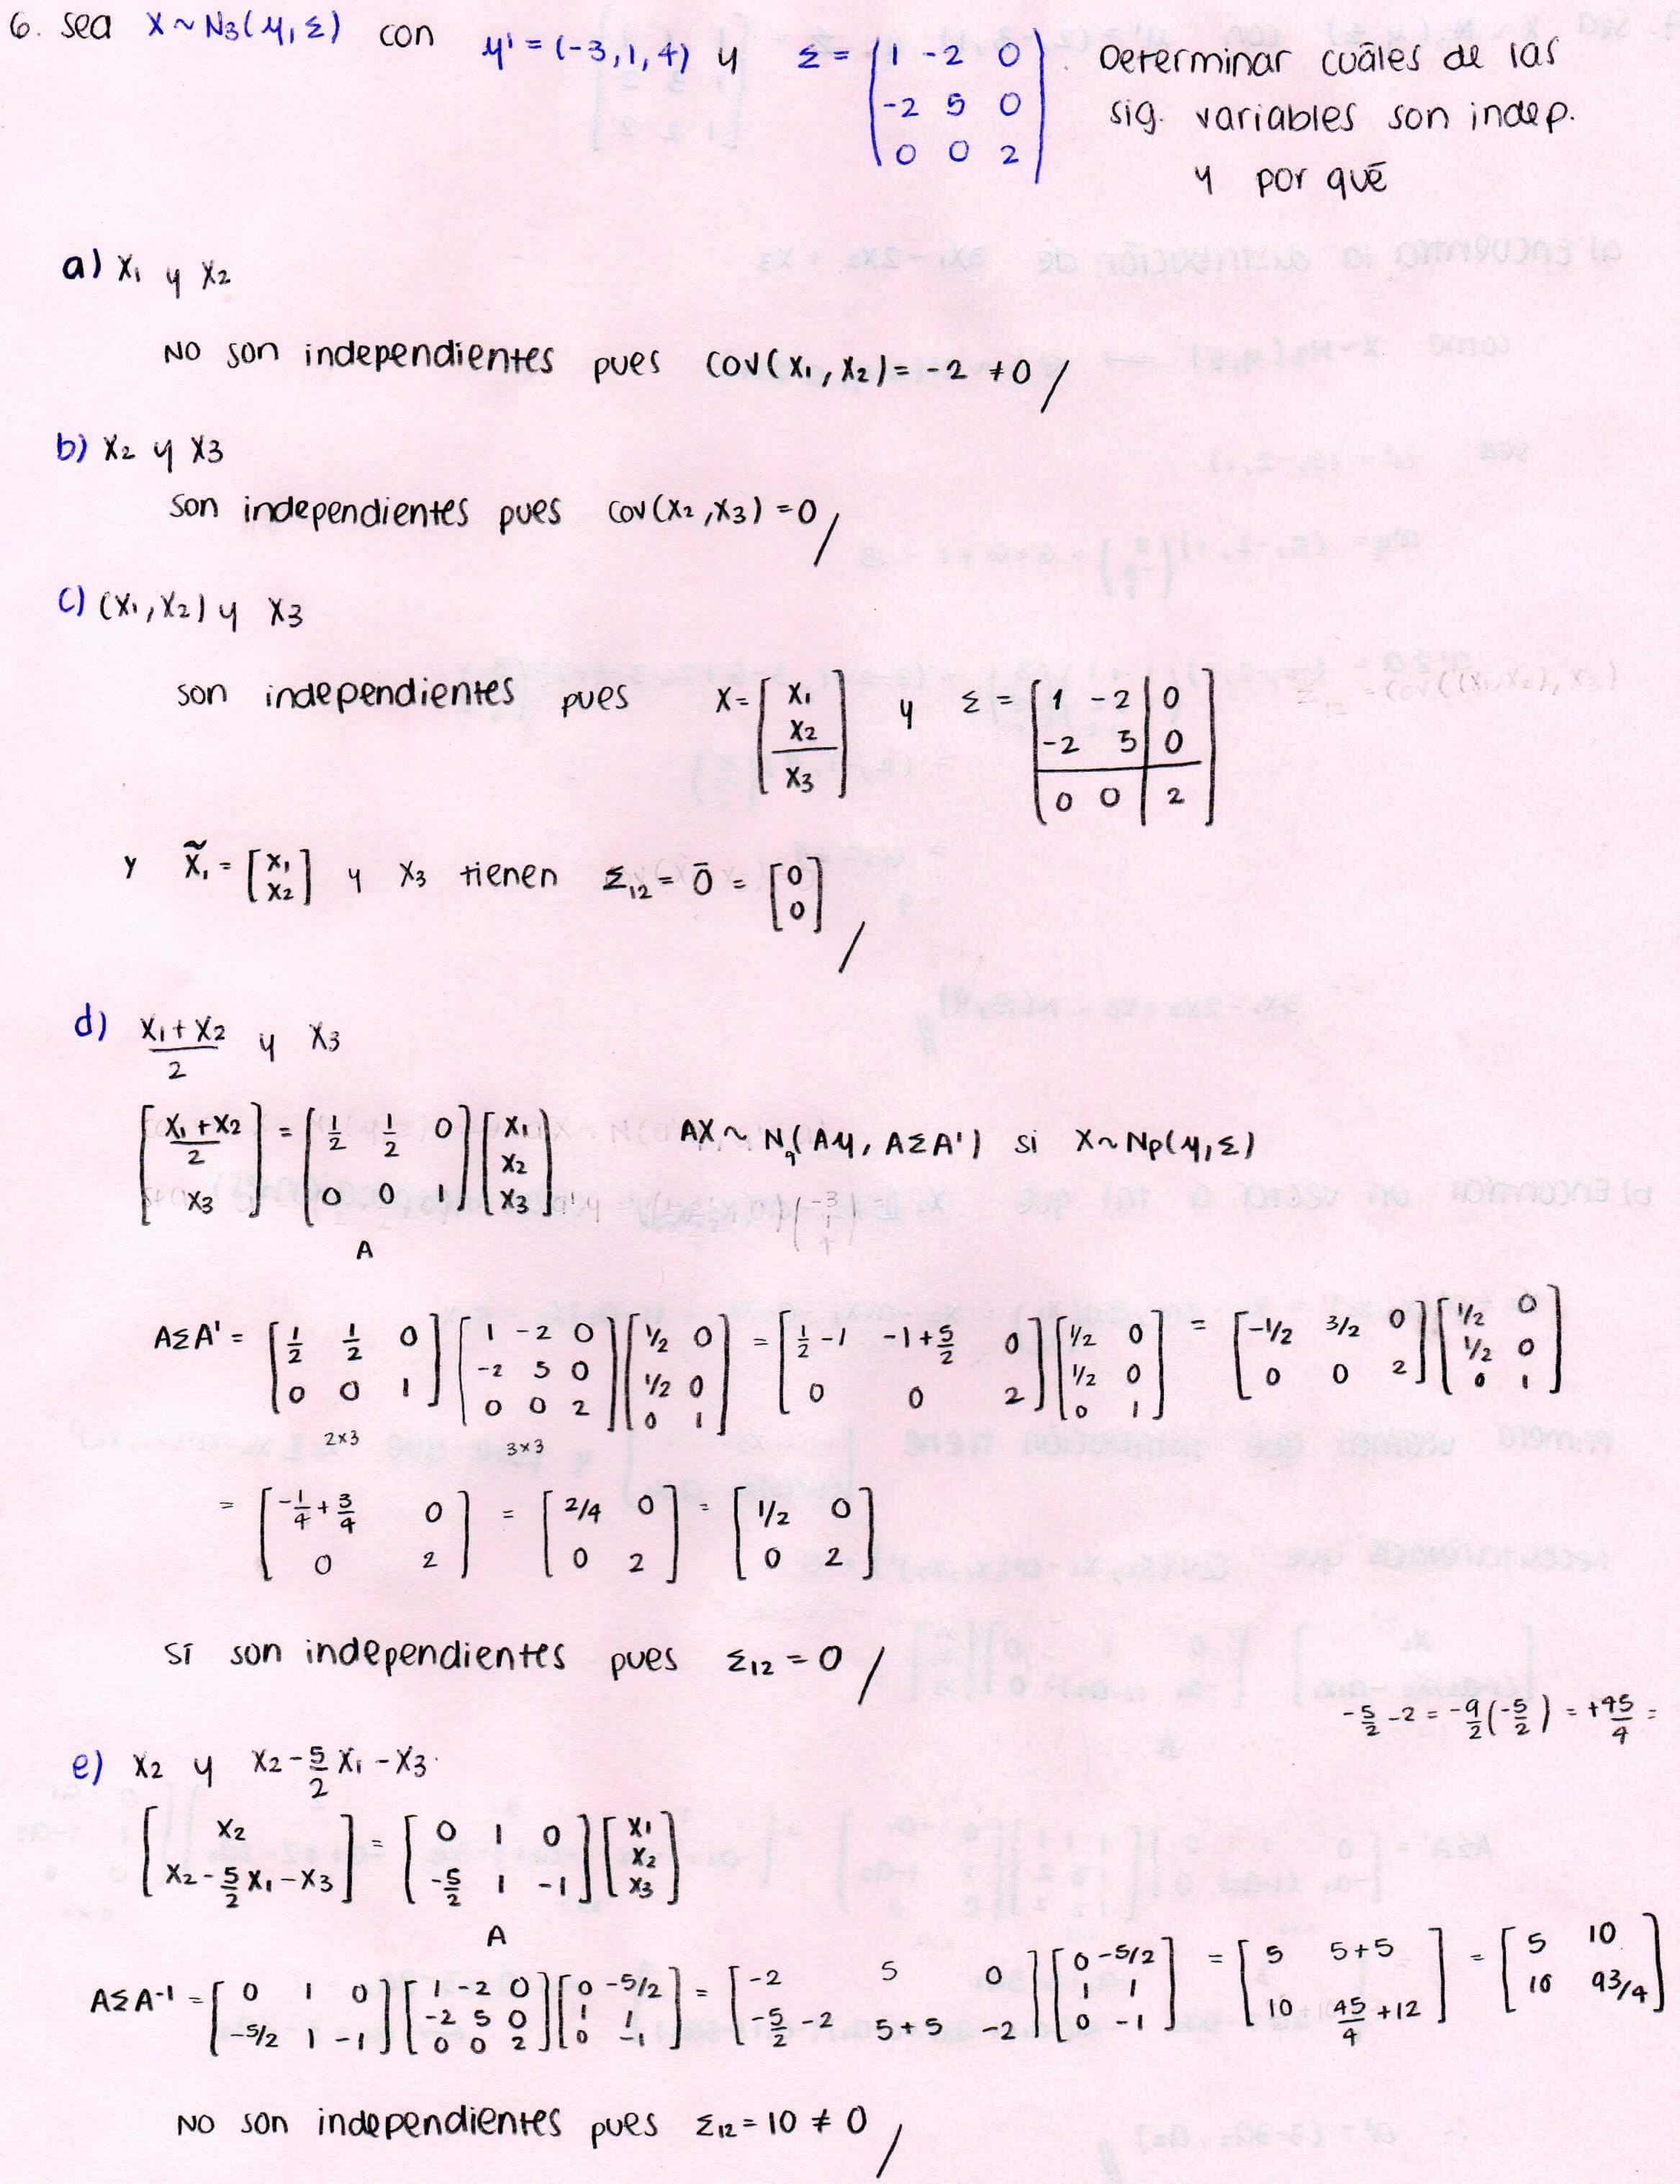
\includegraphics{6.jpg}

\hypertarget{pregunta-7}{%
\subsubsection{\texorpdfstring{\textbf{Pregunta
7}}{Pregunta 7}}\label{pregunta-7}}

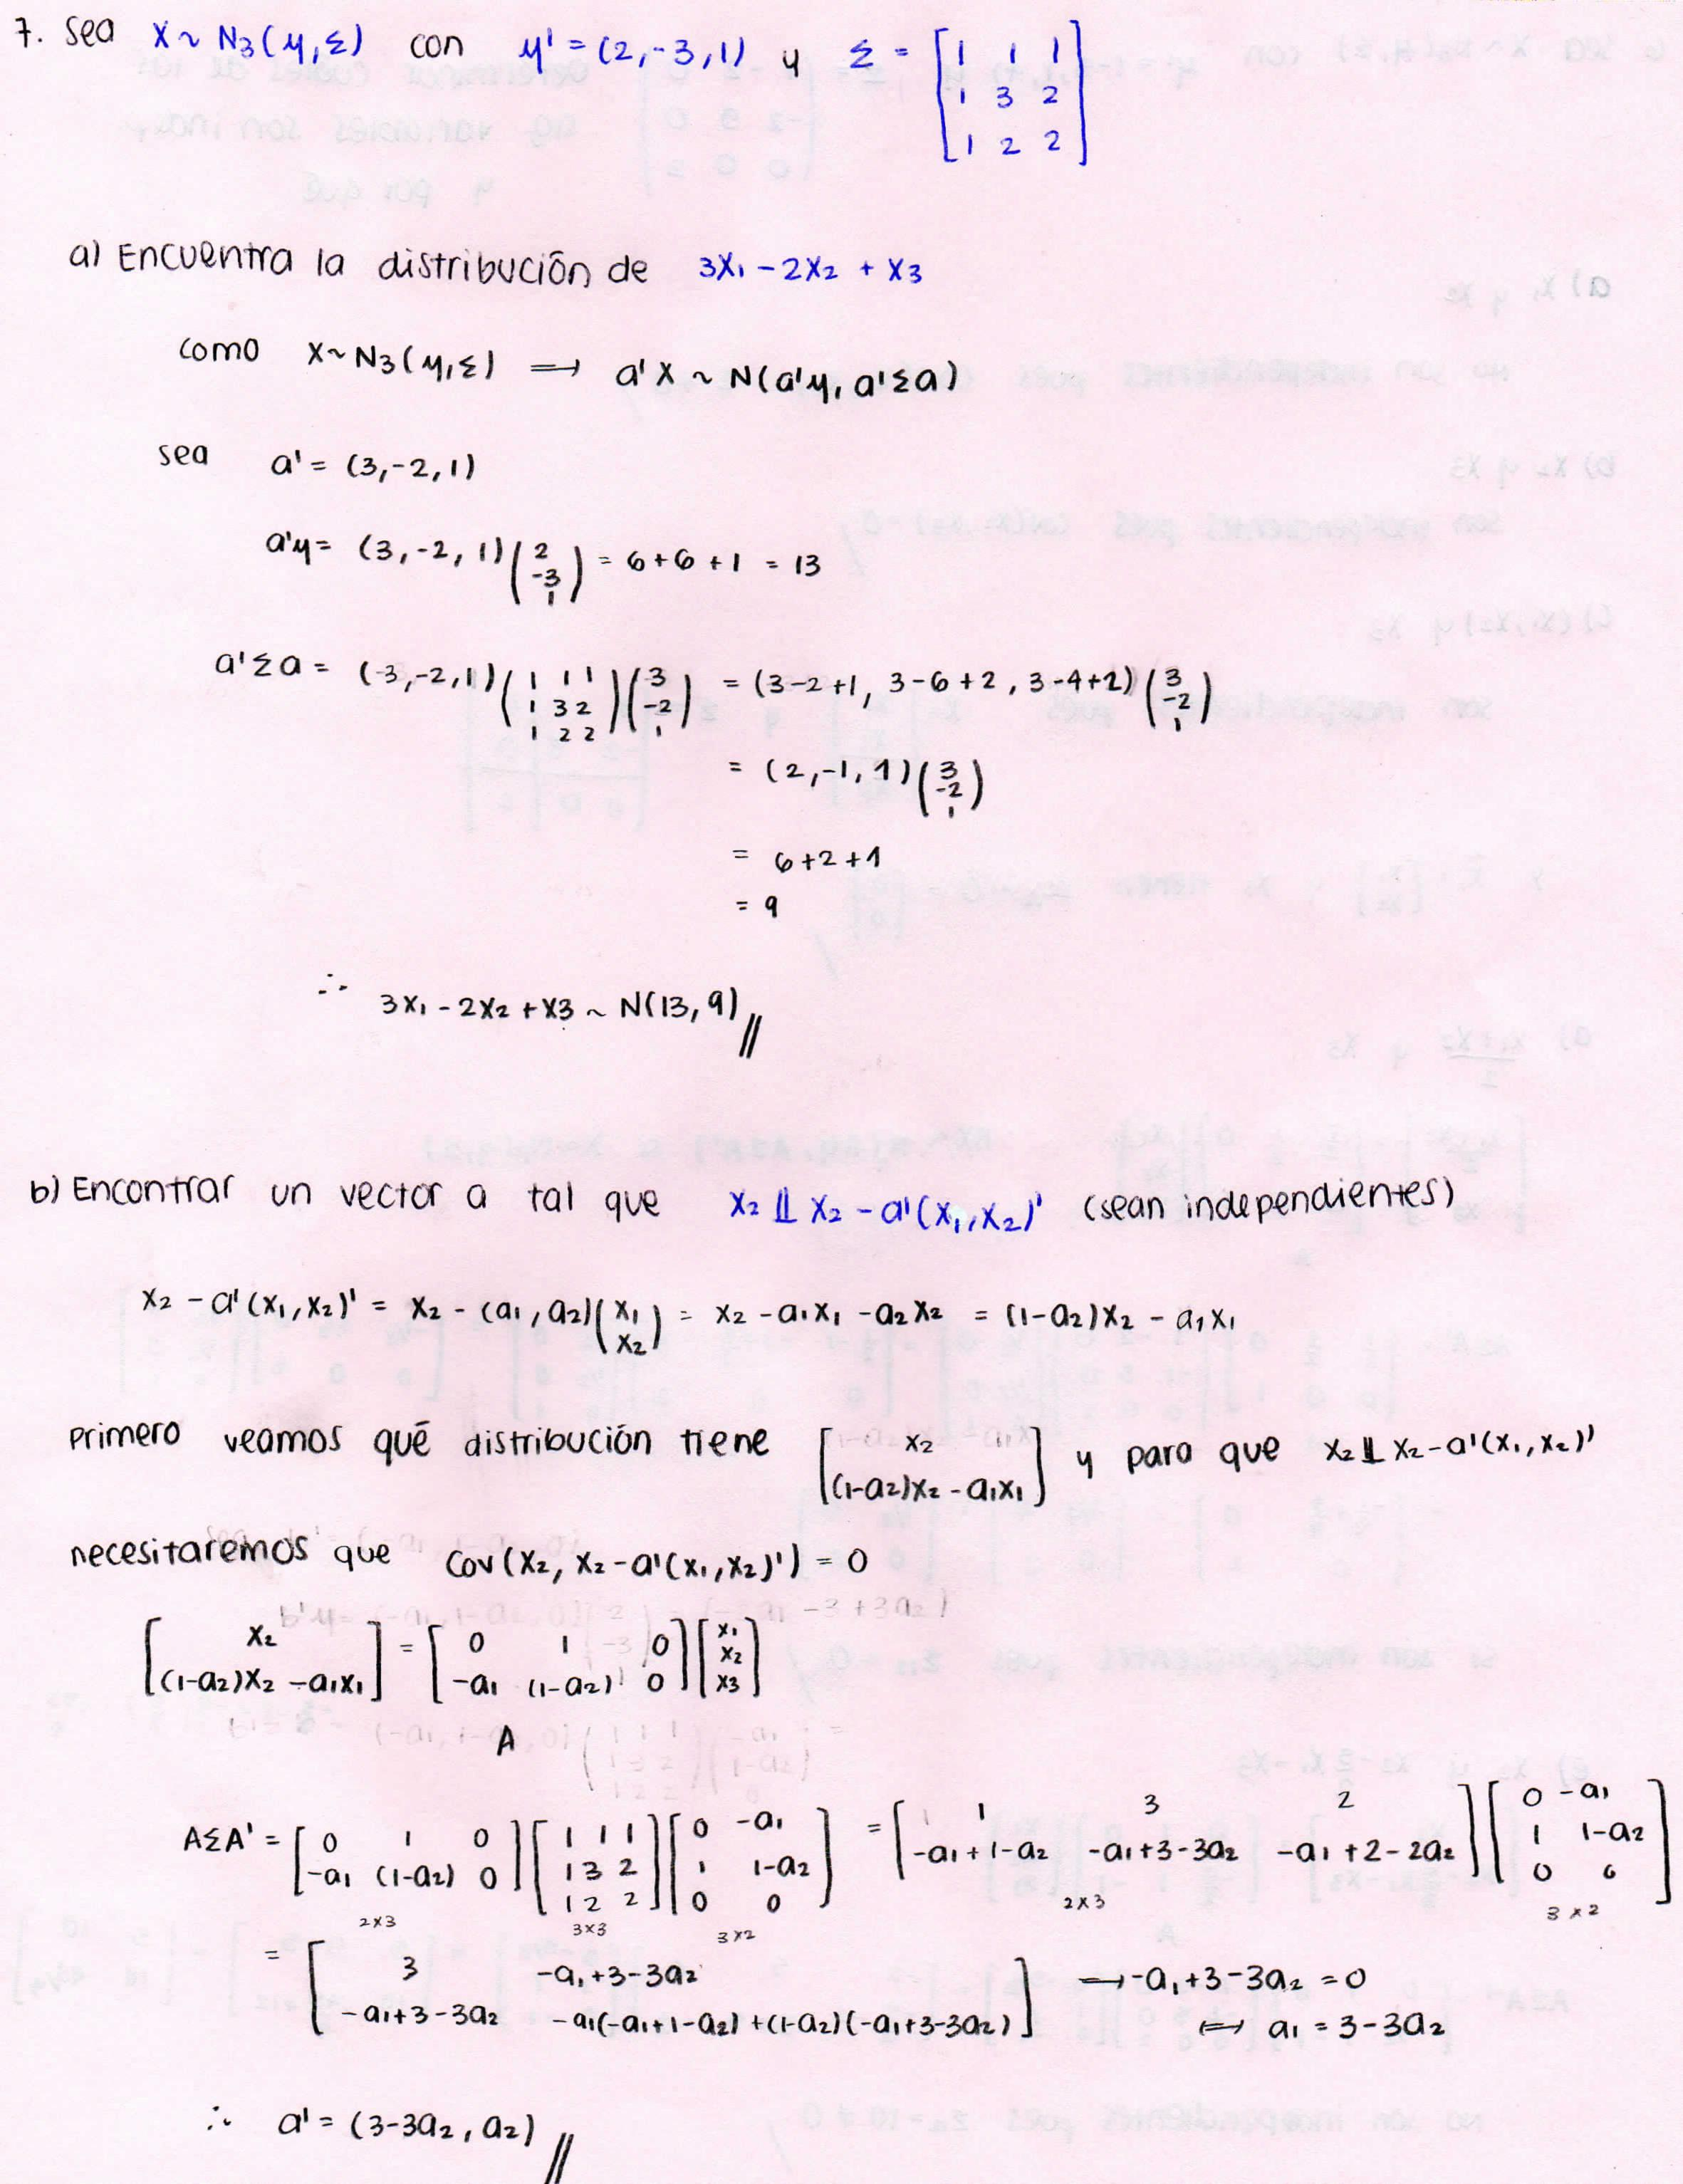
\includegraphics{7.jpg}

\hypertarget{pregunta-8}{%
\subsubsection{\texorpdfstring{\textbf{Pregunta
8}}{Pregunta 8}}\label{pregunta-8}}

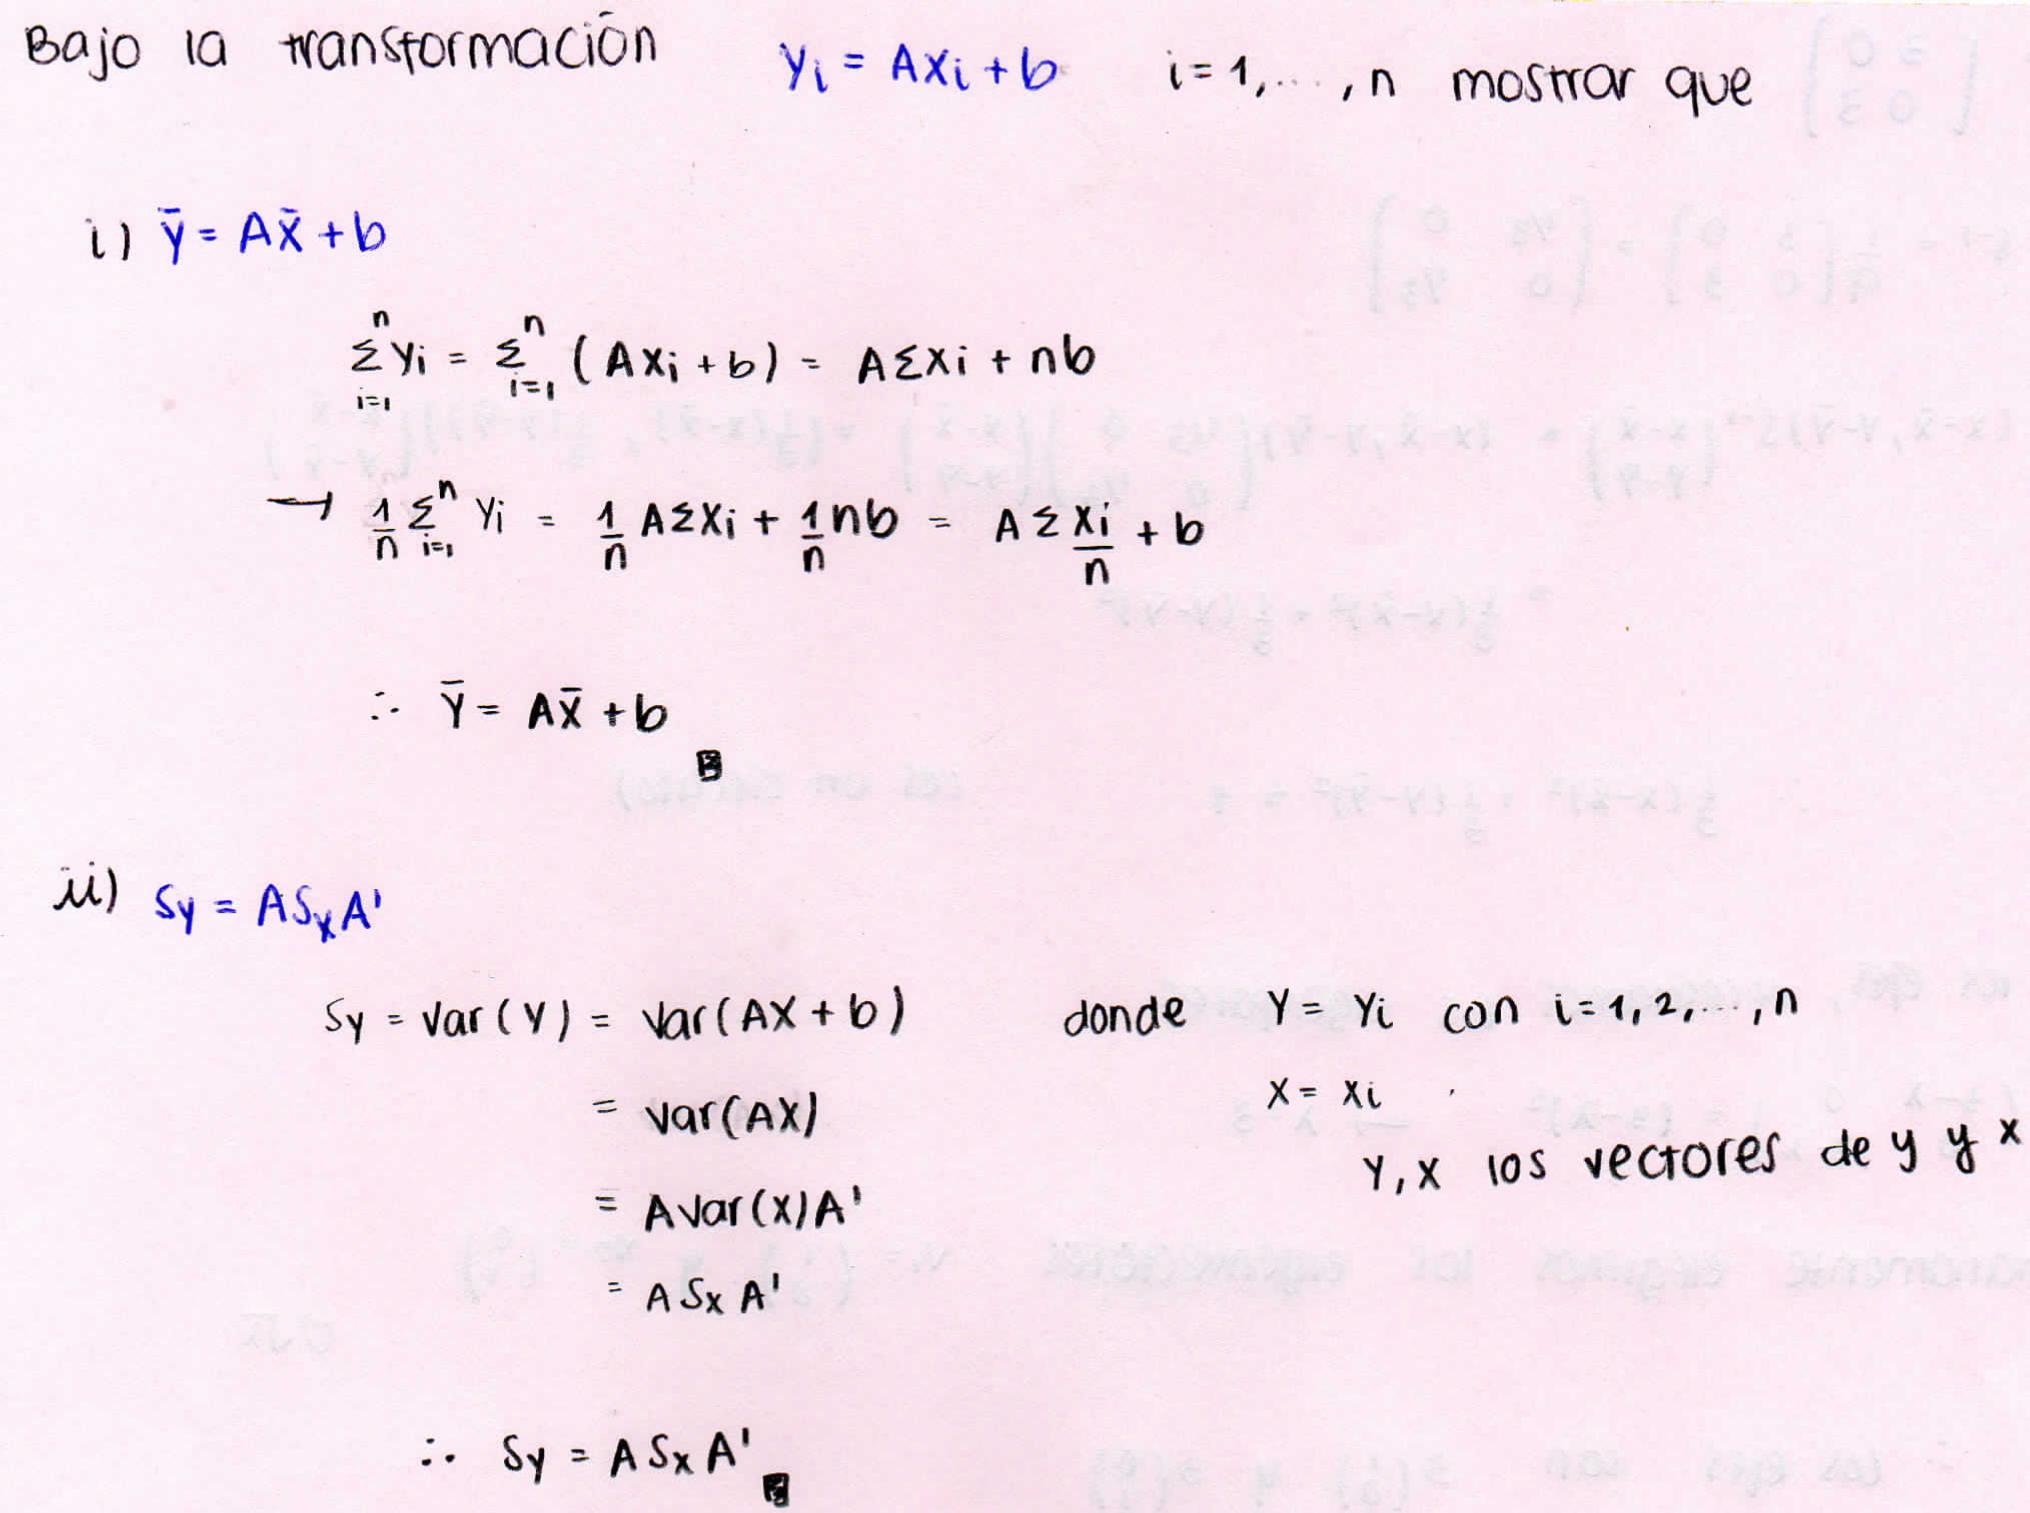
\includegraphics{8.jpg}

\hypertarget{pregunta-9}{%
\subsubsection{\texorpdfstring{\textbf{Pregunta
9}}{Pregunta 9}}\label{pregunta-9}}

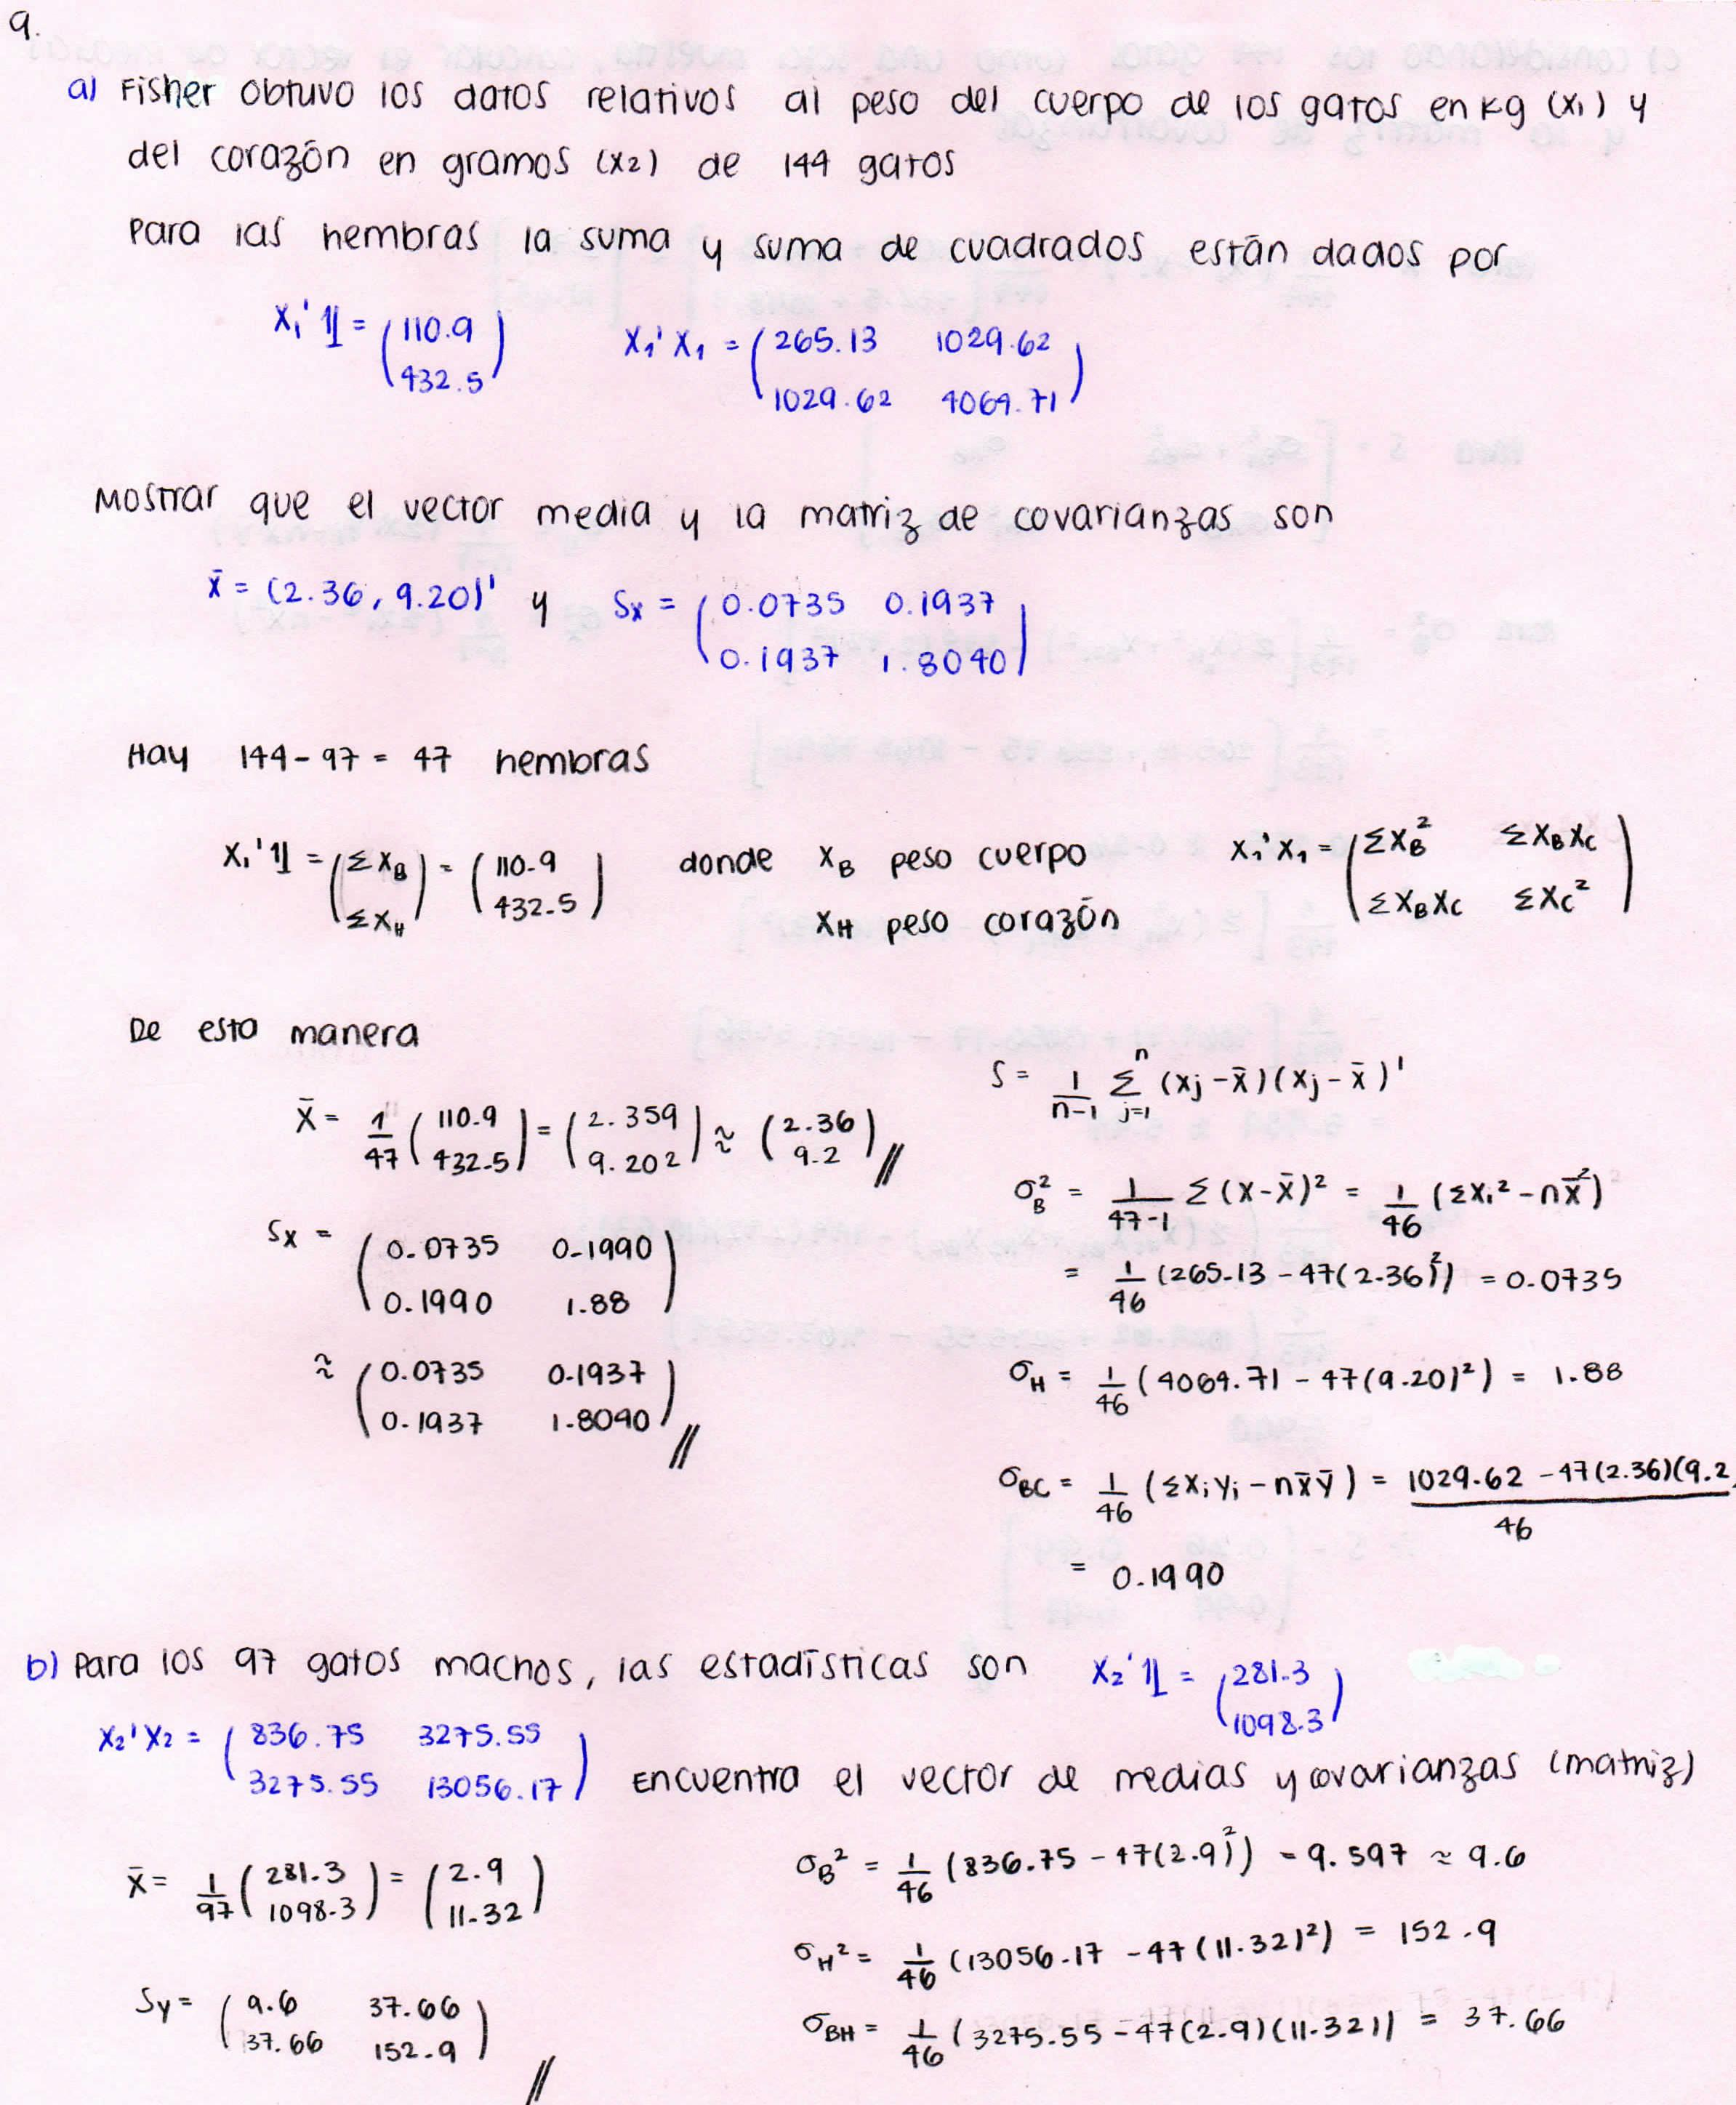
\includegraphics{9a.jpg} 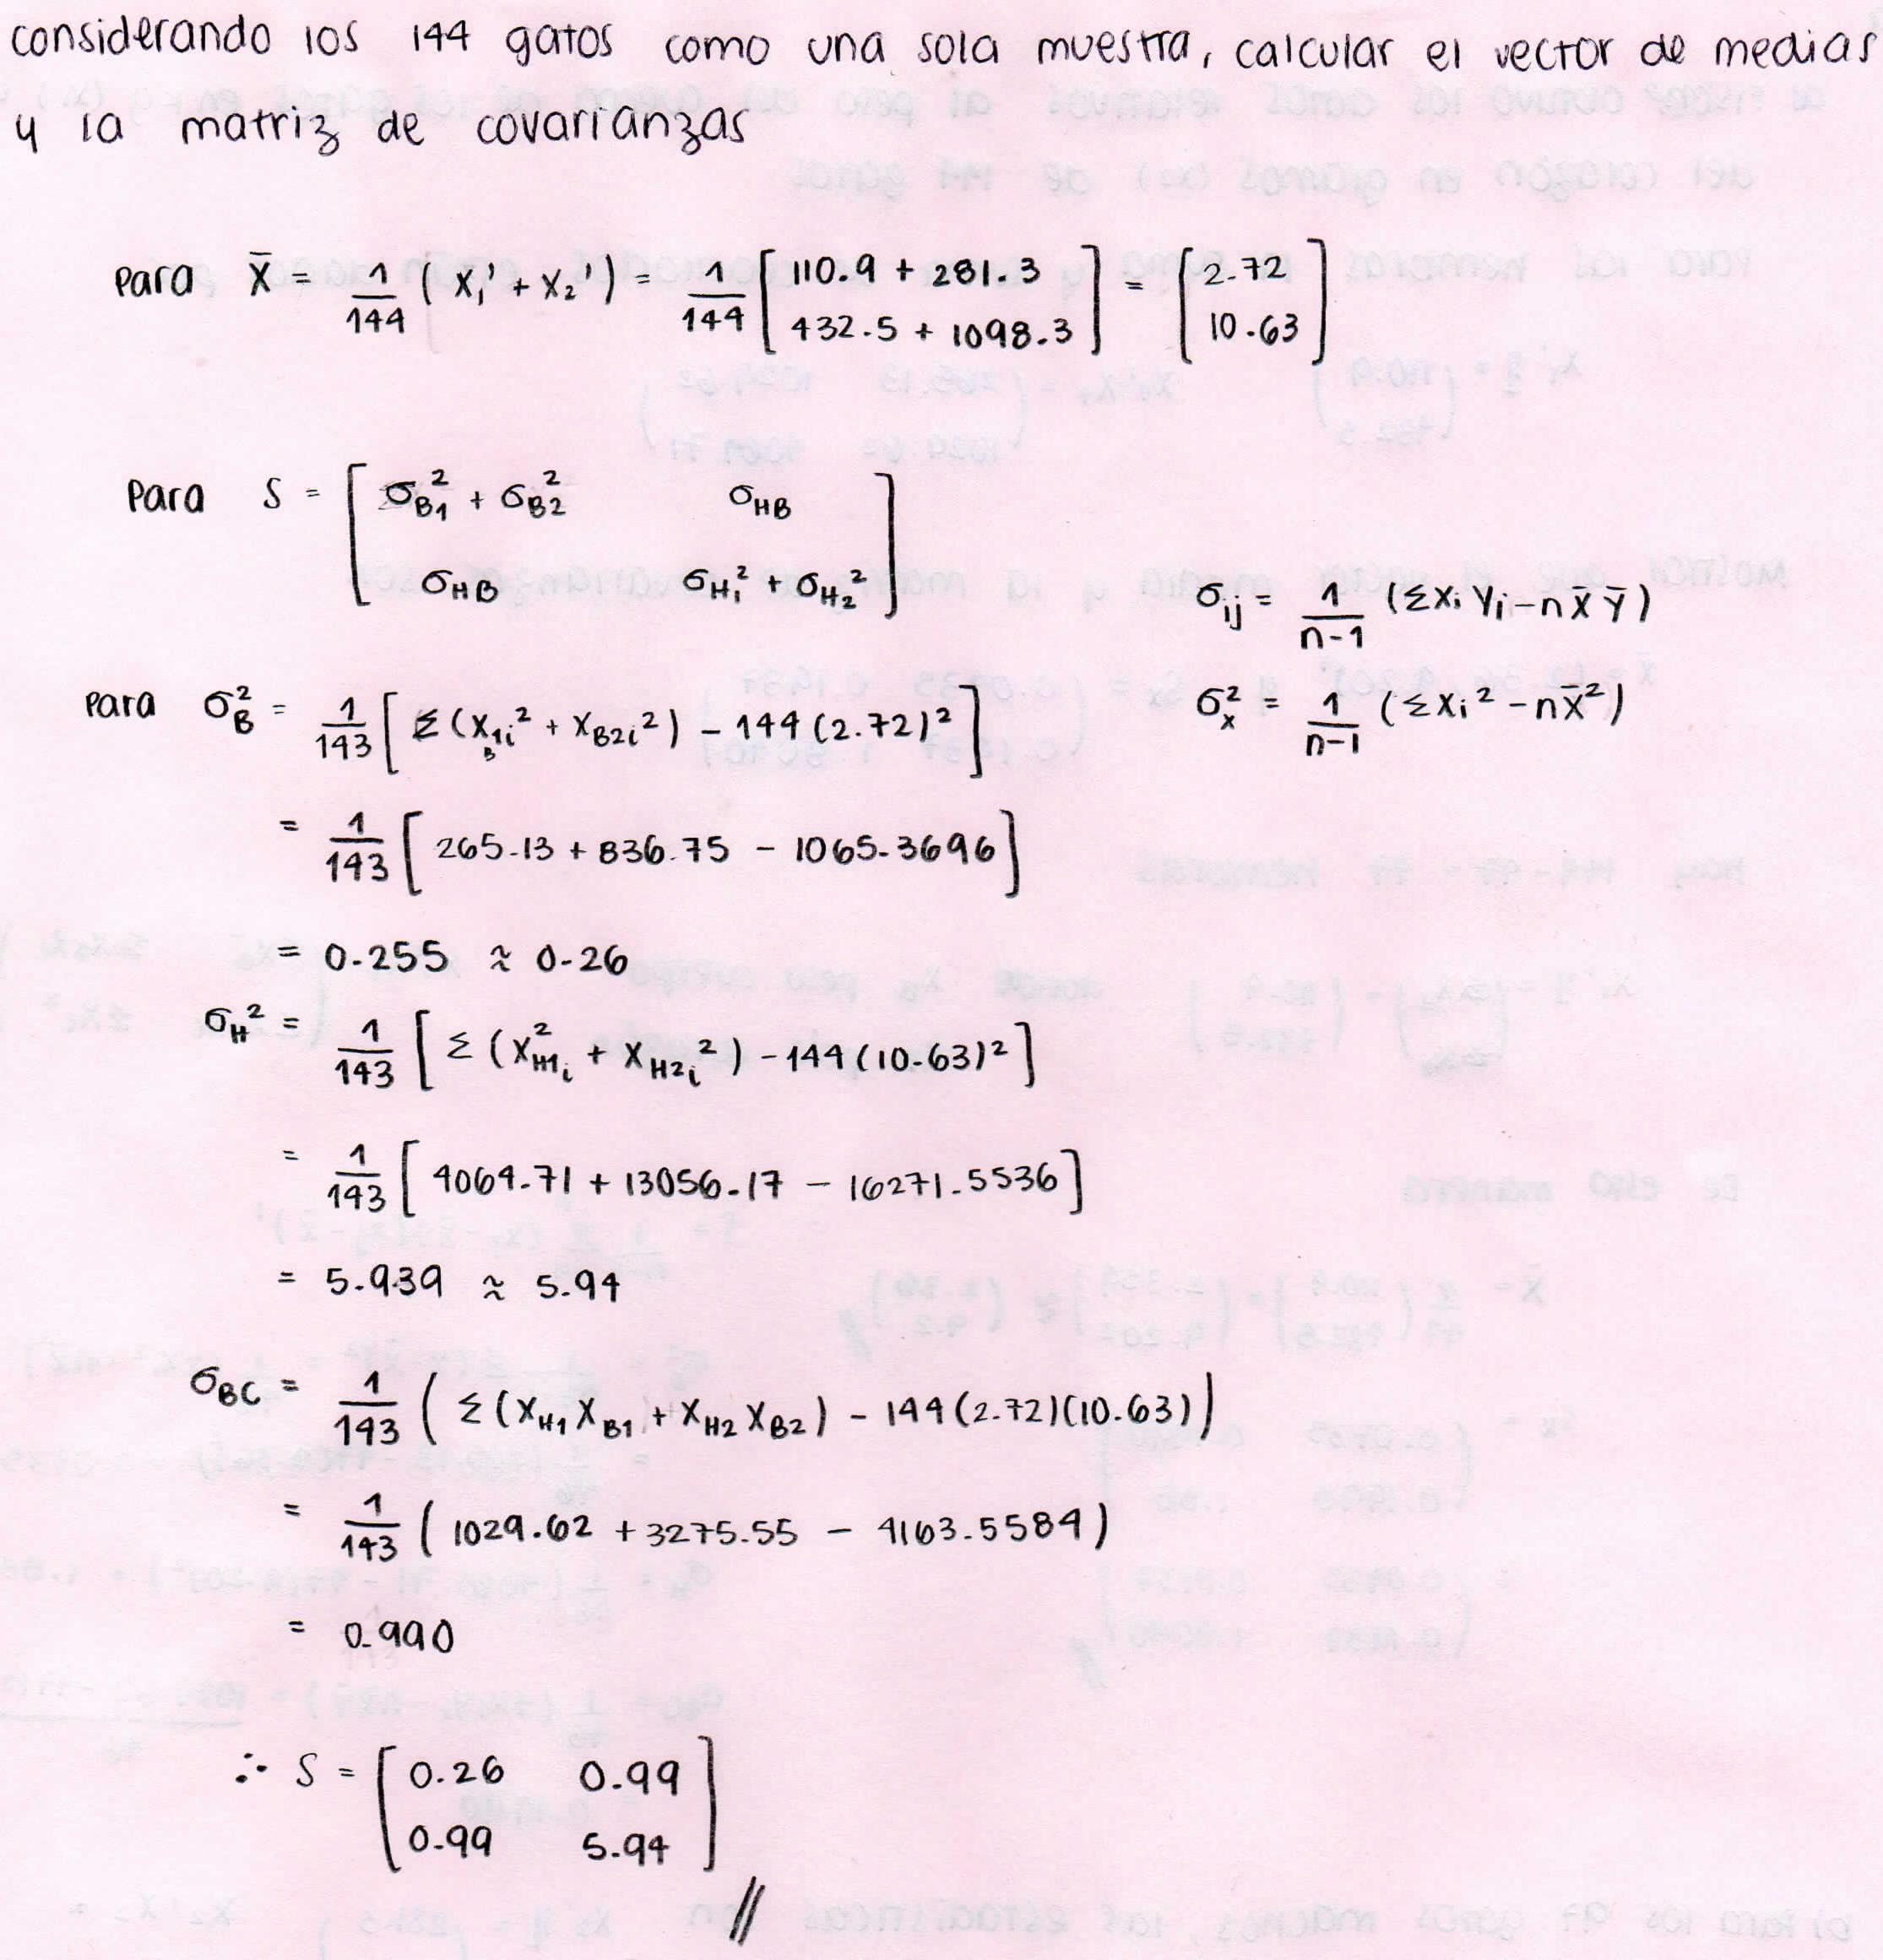
\includegraphics{9b.jpg}
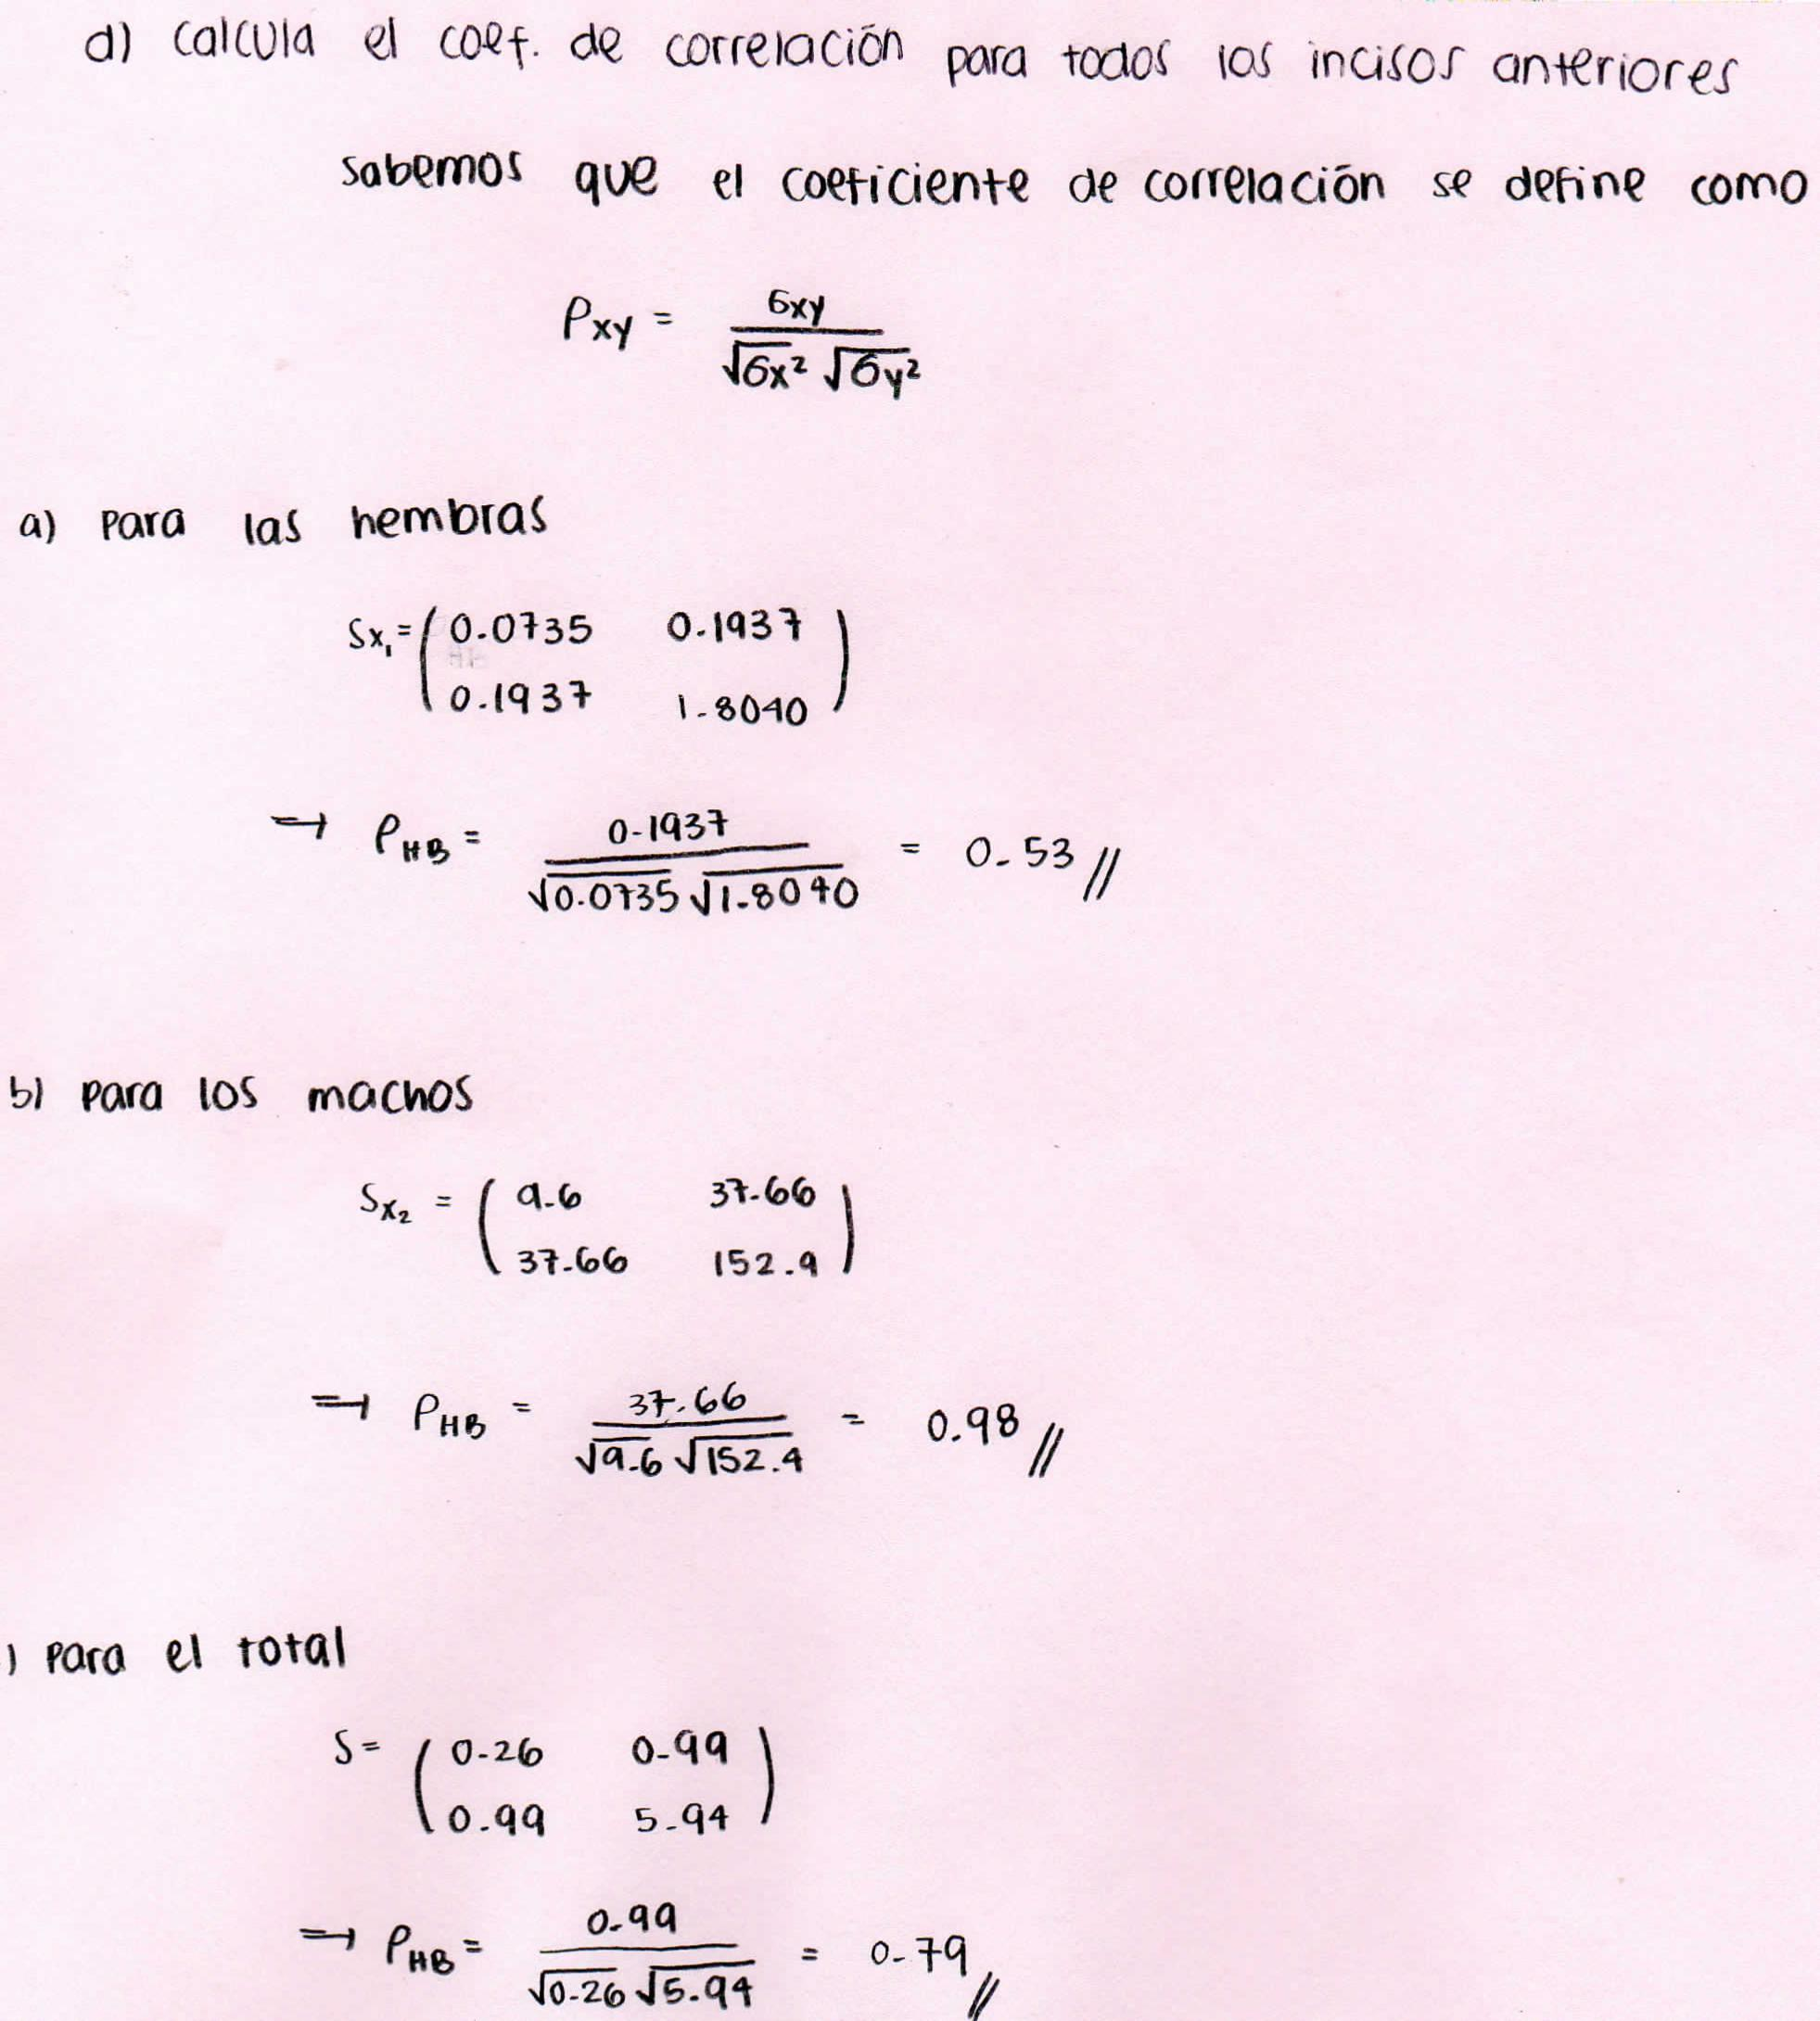
\includegraphics{9c.jpg}

\end{document}
